% vim: tw=0:wrap:linebreak
\documentclass[12pt]{article}

% \setcitestyle{numbers}
\usepackage[numbers]{natbib}
\usepackage[english]{babel}
\usepackage[utf8x]{inputenc}
\usepackage{amsmath}
\usepackage{graphicx}
\usepackage{tabularx}
\usepackage{longtable}
\usepackage[linkcolor=blue,colorlinks=true]{hyperref}
\usepackage{comment}
\usepackage{xspace}
\usepackage[usenames]{xcolor}
\usepackage{datetime}
\usepackage{microtype}
\usepackage{listings}
\usepackage{nameref}

% For referencing {description} environment labels,
% as used in DRP pipeline section.  Taken from
% http://tex.stackexchange.com/questions/1230/reference-name-of-description-list-item-in-latex
\makeatletter
\let\orgdescriptionlabel\descriptionlabel
\renewcommand*{\descriptionlabel}[1]{%
  \let\orglabel\label
  \let\label\@gobble
  \phantomsection
  \edef\@currentlabel{#1}%
  %\edef\@currentlabelname{#1}%
  \let\label\orglabel
  \orgdescriptionlabel{#1}%
}
\makeatother

\newcommand{\vstretch}[1]{\vspace*{\stretch{#1}}}
\newcommand{\code}[1]{\texttt{#1}}

\newcommand{\DIASource}{\code{DIASource}\xspace}
\newcommand{\DIASources}{\code{DIASources}\xspace}
\newcommand{\DIAObject}{\code{DIAObject}\xspace}
\newcommand{\DIAObjects}{\code{DIAObjects}\xspace}
\newcommand{\DB}{{Level 1 database}\xspace}
\newcommand{\DR}{{Level 2 database}\xspace}
\newcommand{\Object}{\code{Object}\xspace}
\newcommand{\Objects}{\code{Objects}\xspace}
\newcommand{\Source}{\code{Source}\xspace}
\newcommand{\Sources}{\code{Sources}\xspace}
\newcommand{\ForcedSource}{\code{ForcedSource}\xspace}
\newcommand{\ForcedSources}{\code{ForcedSources}\xspace}
\newcommand{\CoaddSource}{\code{CoaddSource}\xspace}
\newcommand{\CoaddSources}{\code{CoaddSources}\xspace}
\newcommand{\SSObject}{\code{SSObject}\xspace}
\newcommand{\SSObjects}{\code{SSObjects}\xspace}
\newcommand{\VOEvent}{\code{VOEvent}\xspace}
\newcommand{\VOEvents}{\code{VOEvents}\xspace}
\newcommand{\transSNR}{5\xspace}

% Command to link to a document in Docushare. Pass an LSST document handle as argument, or a document number
\newcommand{\ds}[2]{{\color{blue} \href{https://docushare.lsstcorp.org/docushare/dsweb/Get/#1}{#2}}\xspace}

\newcommand{\SRD}{\ds{LPM-17}{SRD}}
\newcommand{\DPDD}{\ds{LSE-163}{DPDD}}
\newcommand{\LSR}{\ds{LSE-29}{LSR}}
\newcommand{\OSS}{\ds{LSE-30}{OSS}}
\newcommand{\DMSR}{\ds{LSE-61}{DMSR}}
\newcommand{\appsUMLdomain}{\ds{LDM-133}{LDM-133}}
\newcommand{\appsUMLusecase}{\ds{LDM-134}{LDM-134}}
\newcommand{\SUI}{\ds{LDM-131}{SUID}}
\newcommand{\DMSD}{\ds{LDM-148}{DMSD}}
\newcommand{\MOPSD}{\ds{LDM-156}{MOPSD}}
\newcommand{\DMMD}{\ds{LDM-152}{DMMD}}
\newcommand{\DMOps}{\ds{LDM-230}{DM OpsCon}}
\newcommand{\SDQAP}{\ds{LSE-63}{LSE-63}}
\newcommand{\NewPCP}{\ds{LSE-180}{LSE-180}}
\newcommand{\UCAL}{\ds{Document-15125}{UCAL}}

\newcommand{\wbsSFM}{WBS 02C.03.01}
\newcommand{\wbsAssocP}{WBS 02C.03.02}
\newcommand{\wbsAP}{WBS 02C.03.03}
\newcommand{\wbsDiffim}{WBS 02C.03.04}
\newcommand{\wbsMOPS}{WBS 02C.03.06}
\newcommand{\wbsSDQAP}{WBS 02C.01.02.02}
\newcommand{\wbsSDQAT}{WBS 02C.01.02.02}
\newcommand{\wbsSPT}{WBS 02C.01.02.03}
\newcommand{\wbsPSF}{WBS 02C.04.03}
\newcommand{\wbsCoadd}{WBS 02C.04.04}
\newcommand{\wbsDetDeblend}{WBS 02C.04.05}
\newcommand{\wbsObjChar}{WBS 02C.04.06}
\newcommand{\wbsAFW}{WBS 02C.03.05, 02C.04.01}
\newcommand{\wbsCPP}{WBS 02C.04.02}
\newcommand{\wbsPhotoCal}{WBS 02C.03.07}
\newcommand{\wbsAstroCal}{WBS 02C.03.08}




%%% Command's for merging Robert's document, at least temporarily.
%%% Some of these will be removable, some may not be.
\renewcommand{\c}{\textit{c.}\xspace}
\newcommand{\eg}{\textit{e.g.}\xspace}
\newcommand{\etc}{\textit{etc.}\xspace}
\newcommand{\ie}{\textit{i.e.}\xspace}
\renewcommand{\th}{\ensuremath{^{\mbox{\tiny th}}}\xspace}
\newcommand{\Nb}{\textit{N.b.}\xspace}
\newcommand{\nb}{\textit{n.b.}\xspace}
\newcommand{\xib}{{\boldsymbol \xi}}
\newcommand{\zerob}{{\boldsymbol 0}}
%\newcommand{\inputData}[1]{(inputs: \ref{inputs:#1})}
%\newcommand{\inputDataII}[2]{(inputs: \ref{inputs:#1}, \ref{inputs:#2})}
%\newcommand{\outputData}[1]{(calibProducts: \ref{calibProducts:#1})}
%\newcommand{\outputDataII}[2]{(calibProducts: \ref{calibProducts:#1}, \ref{calibProducts:#2})}
%\newcommand{\inputOutputData}[1]{(inputs: \ref{inputs:#1}; calibProducts: \ref{calibProducts:#1})}
%\newcommand{\calypsoData}[1]{(calypsoProducts: \ref{calypso:#1})}
\newcommand{\cameraTeam}{\textbf{Camera Team deliverable}\\}
\newcommand{\TBD}{\textit{T.B.D.}\xspace}
\newcommand{\XXX}[1]{{{\color{red}\textbf{XXX #1}\xspace}}}
\makeatletter
\newcommand{\myLabel}[2]{\def\@currentlabel{#2}\label{#1}}
\makeatother
\newcommand{\appRef}[1]{App. \ref{app:#1}}
\newcommand{\secRef}[1]{Sec. \ref{sec:#1}}
\newcommand{\rednote}[1]{{\color{red} (#1)}}

\newcommand{\alg}{\\ \textbullet\xspace Algorithmic component: }
\newcommand{\fefiftyfive}{$^{55}$Fe\xspace}
\newcommand{\bfeffect}{``brighter-fatter effect"}
\newcommand{\auxtelescope}{auxiliary/Calpyso/calibration telescope\xspace}
\newcommand{\secsymbol}{§}
\newcommand{\xxx}{{\color{red} xxx}\xspace}
\newcommand{\dragons}{ {\color{blue} \textbf{\textit{Here be dragons...}}}}
\newcommand{\mysubitem}{\subitem \textendash\xspace}
\newcommand{\smalltilde}{\raise.26ex\hbox{$\scriptstyle\mathtt{\sim}$}}
\newcommand{\electron}{$e^{-}$}
%%%%%%%%%%%%%%%%%%%%%%%%%%%%%%%%%%%%%%%%%%%



%%%%%%%%%%%%%%%%%%%%%%%%%%%%%%%%%%%%%%%%%%%
%%% Command's for merging Robert's document, at least temporarily.
%\usepackage[top=1cm, bottom=2cm, left=2cm, right=2cm]{geometry} 
%\usepackage{color}
%\usepackage[colorlinks=true, citecolor=blue, linktocpage=true]{hyperref} % n.b. glossary colour is set in style
%\usepackage{enumitem}


\usepackage{titlesec}
%\titleclass{\subsubsubsection}{straight}[\subsection]
%
%\newcounter{subsubsubsection}[subsubsection]
%
%\renewcommand\thesubsubsubsection{\thesubsubsection.\arabic{subsubsubsection}}
%\renewcommand\theparagraph{\thesubsubsubsection.\arabic{paragraph}}
%\renewcommand\thesubparagraph{\theparagraph.\arabic{subparagraph}}
%
%\titleformat{\subsubsubsection}
%{\normalfont\normalsize\bfseries}{\thesubsubsubsection}{1em}{}
%\titlespacing*{\subsubsubsection}
%{0pt}{3.25ex plus 1ex minus .2ex}{1.5ex plus .2ex}


%\usepackage[style=authoryear, uniquename=false, backend=biber]{biblatex}
%\usepackage{amsmath} %maths
%\usepackage{graphicx}
%\usepackage{import}
%\usepackage{xspace}
%\usepackage{perpage}
%

%%%%%%%%%%%%%%%%%%%%%%%%%%%%%%%%%%%%%%%%%%%


\newenvironment{note}[1][Note]
{
  \begin{displaymath}
    \left[ \qquad
    \begin{minipage}[h]{.75\linewidth}
      \color{red} \footnotesize
      \textbf{#1:} \newline
      \color{black}
}
{
    \end{minipage}
    \normalsize
    \qquad \right]
  \end{displaymath}
}

\newcommand{\uc}[1]{{\tt #1}}

\setcounter{secnumdepth}{5}
\setcounter{tocdepth}{5}

\title{Large Synoptic Survey Telescope \\
Data Management Applications Design \\
{\author{
    M. Juri\'c\footnote{Please direct comments to \textless\href{mailto:mjuric@lsst.org}{mjuric@lsst.org}\textgreater.},
                     R.H. Lupton, T. Axelrod, A.C. Becker, J. Becla,  \\
    J.F. Bosch,  D.R. Ciardi,  A.J. Connolly,  G.P. Dubois-Felsmann, \\ 
    F. Economou, M. Fisher-Levine, \v{Z}. Ivezi\'c,  M. Graham, \\
    T. Jenness,  R.L. Jones, J. Kantor, S. Krughoff, K-T Lim, \\
    P.A. Price,  D. Shaw,  C. Slater, J. Swinbank, \\
    {\em for the LSST Data Management}
}}}

 
\begin{document}
\date{\today, \currenttime hrs}
\maketitle
\pagestyle{headings}

\begin{abstract}
The LSST Science Requirements Document (the LSST \SRD) specifies a set of
data product guidelines, designed to support science goals envisioned to be enabled by the LSST observing program. Following these guidlines, the details of these data products have been described in the LSST Data Products Definition Document (\DPDD), and captured in a formal flow-down from the \SRD via the LSST System Requirements (\LSR), Observatory System Specifications (\OSS), to the Data Management System Requirements (\DMSR).
The LSST Data Management subsystem's responsibilities include the design, implementation, deployment and execution of software pipelines necessary to generate these data products. This document, in conjunction with the UML Use Case model (\appsUMLusecase), describes the design of the scientific aspects of those pipelines.
\end{abstract}


\tableofcontents

\section{Preface}

The purpose of this document is to describe the design of pipelines belonging to the Applications Layer of the Large Synoptic Survey Telescope (LSST) Data Management system. These include most of the core astronomical data processing software that LSST employs.

The intended audience of this document are LSST software architects and developers. It presents the baseline architecture and algorithmic selections for core DM pipelines. The document assumes the reader/developer has the required knowledge of astronomical image processing algorithms and solid understanding of the state of the art of the field, understanding of the LSST Project goals and concepts, and has read the LSST Science Requirements (\SRD) as well as the LSST Data Products Definition Document (\DPDD).

This document should be read in conjunction with the LSST DM Applications Use Case Model (\appsUMLusecase). They are intended to be complementary, with the Use Case model capturing the detailed (inter)connections between individual pipeline components, and this document capturing the overall goals, pipeline architecture, and algorithmic choices.

Though under strict change control\footnote{LSST Docushare handle for this document is {\tt LDM-151}.}, this is a {\bf \em living document}. Firstly, as a consequence of the ``rolling wave" LSST software development model, the designs presented in this document will be refined and made more detailed as particular pipeline functionality is about to be implemented. Secondly, the LSST will undergo a period of construction and commissioning lasting no less than seven years, followed by a decade of survey operations. To ensure their continued scientific adequacy, the overall designs and plans for LSST data processing pipelines will be periodically reviewed and updated.


\section{Introduction}

\subsection{LSST Data Management System}

To carry out this mission the Data Management System (DMS) performs the following major functions:

\begin{itemize}
\item Processes the incoming stream of images generated by the camera
  system during observing to produce transient alerts and to archive
  the raw images.

\item Roughly once per year, creates and archives a Data Release (``DR''),
  which is a static self-consistent collection of data products
  generated from all survey data taken from the date of survey
  initiation to the cutoff date for the Data Release. The data
  products (described in detail in the \DPDD), include measurements of 
  the properties (shapes, positions, fluxes, motions, etc.) of all detected
  objects, including those below the single visit sensitivity limit,
  astrometric and photometric calibration of the full survey object
  catalog, and limited classification of objects based on both their
  static properties and time-dependent behavior.  Deep coadded images
  of the full survey area are produced as well.

\item Periodically creates new calibration data products, such as bias
  frames and flat fields, that will be used by the other processing
  functions, as necessary to enable the creation of the data products above.

\item Makes all LSST data available through interfaces that utilize,
  to the maximum possible extent, community-based standards such as those
  being developed by the Virtual Observatory (``VO''), and facilitates user
  data analysis and the production of user-defined data products at Data
  Access Centers (``DAC'') and at external sites.
\end{itemize}

The overall architecture of the DMS is discussed in more detail in the Data Management System Design (\DMSD) document. The overall architecture of the DMS is shown in Figure~\ref{fig:DMS}.
\\

This document discusses the role of the Applications layer in the first three functions listed above (the functions involving \emph{science pipelines}).  The fourth is discussed separately in the SUI Conceptual Design Document (\SUI).

\begin{figure}
\centering
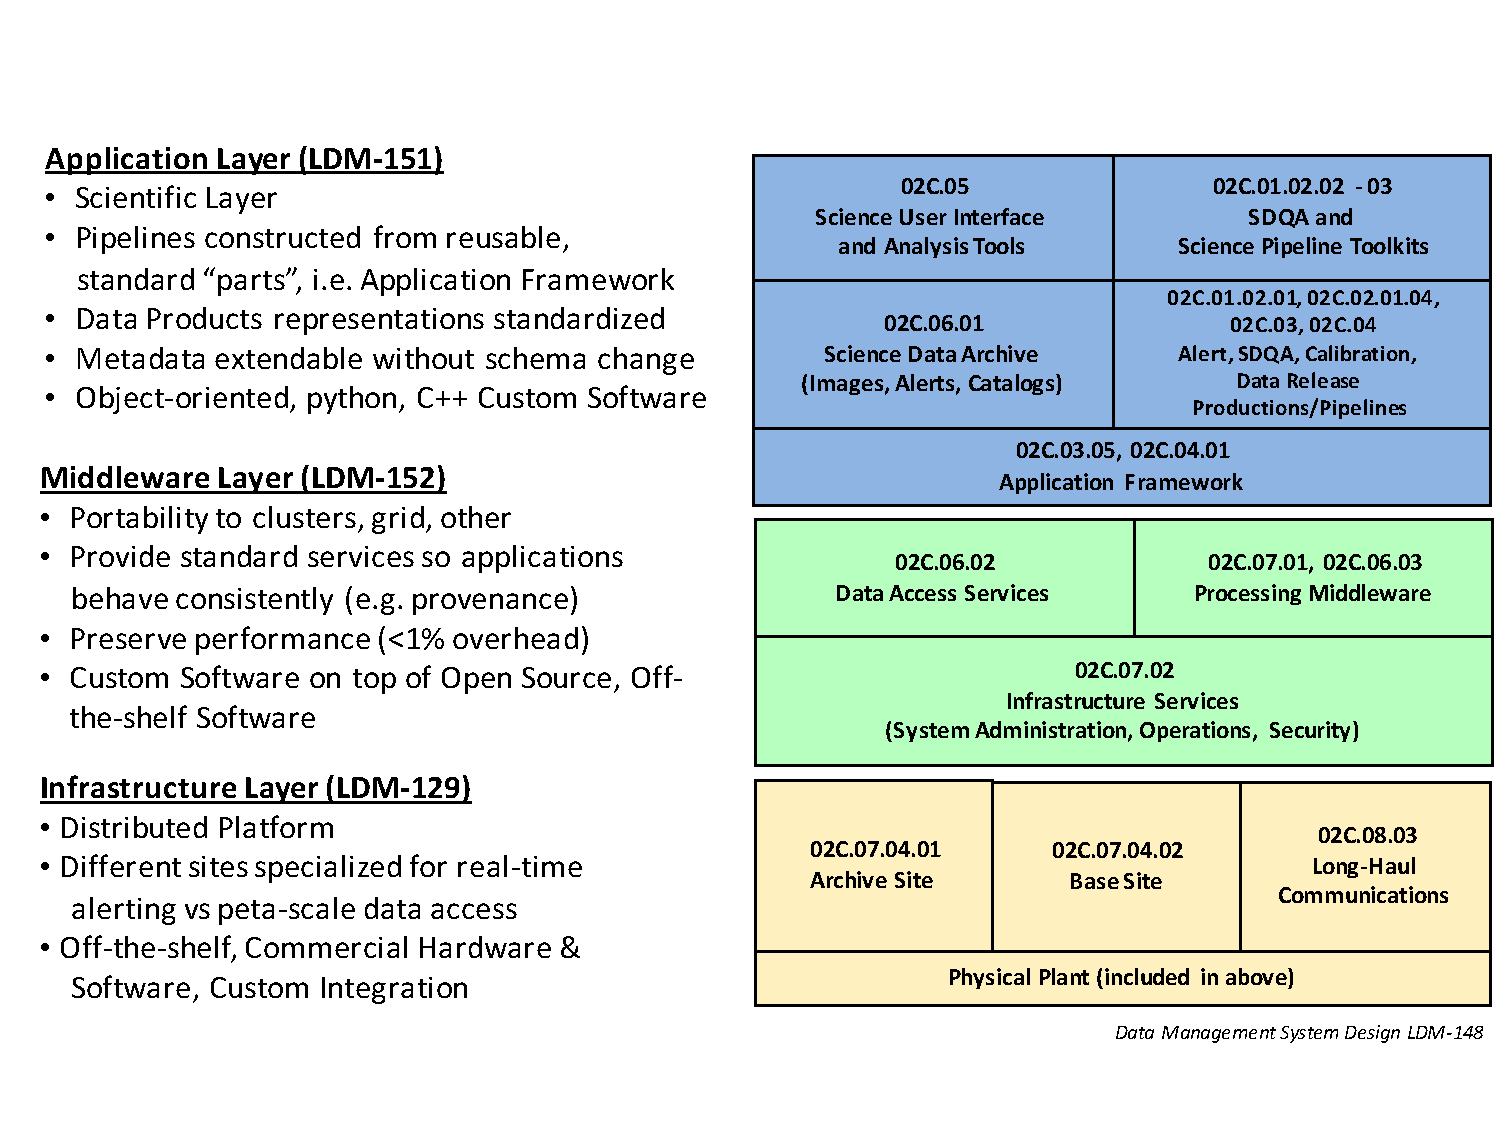
\includegraphics[angle=90,scale=0.70]{figures/DMS-Architecture.pdf}
\caption{Architecture of the Data Management System\label{fig:DMS}}
\end{figure}

\begin{figure}
%\includegraphics[angle=90,scale=0.70]{ApplicationLayerProductionsandPipelines.eps}
\centering
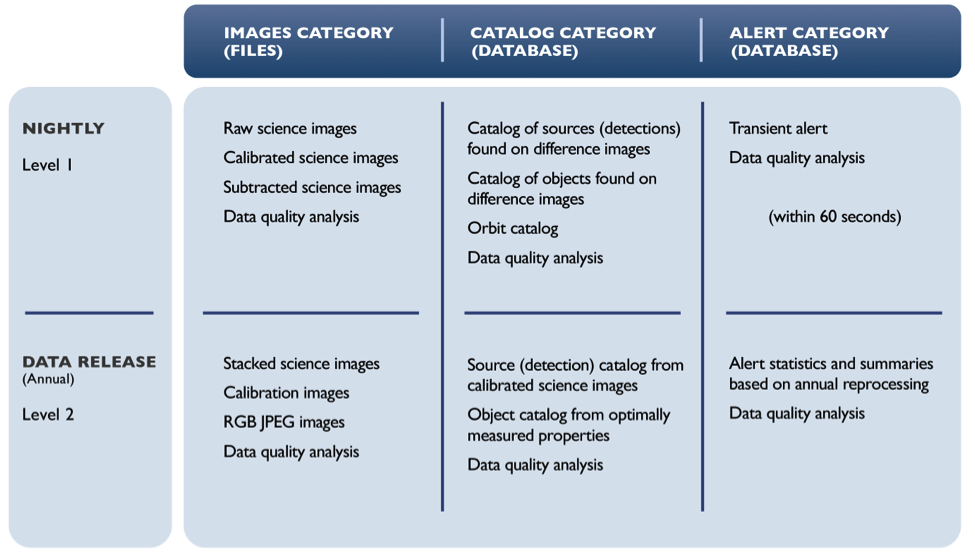
\includegraphics[angle=90]{figures/DataProductDelivarables.png}
\caption{Organization of LSST Data Products\label{fig:DP}}
\end{figure}

\subsection{Data Products}

The LSST data products are organized into three groups, based on their intended use and/or origin. The full description is provided in the Data Products Definition Document (\DPDD); we summarize the key properties here to provide the necessary context for the discussion to follow. 

\begin{itemize}
\item {\bf Level 1} products are intended to support timely detection and follow-up
  of time-domain events (variable and transient sources). They are generated by
  near-real-time processing the stream of data from the camera system during 
  normal observing.  Level 1 products are therefore continuously generated and / or
  updated every observing night. This process is of necessity highly
  automated, and must proceed with absolutely minimal human
  interaction.  In addition to science data products, a number of related
  Level 1 ``SDQA''\footnote{Science Data Quality Analysis} data products are generated
  to assess quality and to provide feedback to the Observatory Control System (OCS).

\item {\bf Level 2} products are generated as part of a Data Release, generally
  performed 
  yearly, with an additional data release for the first 6 months of survey data. 
  Level 2 includes data products for which extensive
  computation is required, often because they combine information from
  many exposures.  Although the steps that generate Level 2 products
  will be automated, significant human interaction may be required at
  key points to ensure the quality of the data.

\item {\bf Level 3} products are generated on any computing resources
  anywhere and then stored in an LSST Data Access Center. Often, but not
  necessarily, they will be generated by users of LSST using LSST software
  and/or hardware. LSST DM is required to facilitate the creation of
  Level 3 data products by providing suitable APIs, software components, and
  computing infrastructure, but will not by itself create any Level 3
  data products. Once created, Level 3 data products may be associated with
  Level 1 and Level 2 data products through database federation.
  Where appropriate, the LSST Project, with the agreement of the Level 3
  creators, may incorporate user-contributed Level 3 data product pipelines
  into the DMS production flow, thereby promoting them to Level 1 or 2.

\end{itemize}

The organization of LSST Data Products is shown in Figure~\ref{fig:DP}.

Level 1 and Level 2 data products that have passed quality control
tests will be accessible to the public without restriction.
Additionally, the source code used to generate them will be made
available, and LSST will provide support for builds on selected
platforms.

The pipelines used to produce these public data products will also produce many intermediate data products that may not be made publically available (generally because they are fully superseded in quality by a public data product).  Intermediate products may be important for QA, however, and their specification is an important part of describing the pipelines themselves.

\subsection{Data Units}

In order to describe the components of our processing pipelines, we first need standard nomenclature for the units of data the pipeline will process.

The smallest data units are those corresponding to individual astrophysical entities.  In keeping with LSST conventions, we use ``object'' to refer to the astrophysical entity itself (which typically implies aggregation of some sort over all exposures), and ``source'' to refer to the realization of an object on a particular exposure.  In the case of blending, of course, these are just our best attempts to define distinct astrophysical objects, and hence it is also useful to define terms that represent this process.  We use ``family'' to refer to group of blended objects (or, more rarely, sources), and ``child'' to refer to a particular deblended object within a family.  A ``parent'' is also created for each family, representing the alternate hypothesis that the blend is actually a single object.  Blends may be hierarchical; a child at one level may be a parent at the level below.

LSST observations are taken as a pair of 15-second ``snaps''; together these constitute a ``visit''.  Because snaps are typically combined early in the processing (and some special programs and survey modes may take only a single snap), visit is much more frequently used as a unit for processing and data products.  The image data for to a visit is a set of 189 ``CCD'' or ``sensor'' images.  CCD-level data from the camera is further data divided across the 16 amplifiers within a CCD, but these are also combined at an early stage, and the 3$\times$3 CCD ``rafts'' that play an important role in the hardware design are relativley unimportant for the pipeline.  This leaves visit and CCD the main identifiers of most exposure-level data products and pipelines.

Our convention for defining regions on the sky is deliberately vague; we hope to build a codebase capable of working with virtually any pixelization or projection scheme (though different schemes may have different performance or storage implications).  Our approach involves two region concepts: ``tracts'' and ``patches''.  A tract is a large region with a single Cartesian coordinate system; we assume it is larger than the LSST field of view, but its maximum size is essentially set by the point at which distortion in the projection becomes significant enough to affect the processing (by e.g. breaking the assumption that the PSF is well-sampled on the pixel grid).  Tracts are divided into patches, all of which share the tract coordinate system.  Most image processing is perfomed at the patch level, and hence patch sizes are chosen largely to ensure that patch-level data products and processing fit in memory.  Both tracts and patches are defined such that each region overlaps with its neighbors, and these overlap regions must be large enough that any individual astronomical object is wholly contained in at least one tract and patch.  In a patch overlap region, we expect pixel values to be numerically equivalent (i.e. equal up to floating point round-off errors) on both sides; in tract overlaps, this is impossible, but we expect the results to be scientifically consistent.  Selecting larger tracts and patches thus reduces the overall fraction of the area that falls in overlap regions and must be processed multiple times, while increasing the computational load for processing individual tracts and patches.

\subsection{Science Pipelines Organization}

As shown in Figure~\ref{fig:DMS}, the Applications Layer is itself split into three levels.  In sections~\ref{sec:ap}, \ref{sec:cpp}, and \ref{sec:drp}, we describe the Alert Production, Calibration Products Production, and Da
ta Release Production (respectively), breaking them down into \emph{pipelines}.  In this document, a pipeline is a high-level combination of algorithms that is intrinsically tied to its role in the production in which it is run.  For instance, while both Alert Production and Data Release Production will include a pipeline for single-visit processing, these two pipelines are \emph{distinct}, because the details of their design depend very much on the context in which they are run.  Section~\ref{sec:sdqa} describes the Science Data Quality Analysis System, a collection of pipelines and mini-productions designed to assess and continuously validate the quality of both the data and the processing system.  The SDQA System is not a single production; its components are either directly integrated into other productions or part of a set of multiple mini-productions run on different cadences.

Pipelines are largely composed of Algorithmic Components: mid-level algorithmic code that we expect to reuse (possibly with different configuration) across different productions.  These components constitute the bulk of the new code and algorithms to be developed for Alert Production and Data Release Production, and are discussed in section~\ref{sec:algorithmic-components}.  Most algorithmic components are applicable to any sort of astronomical imaging data, but some will be customized for LSST.

The lowest level in the Applications Layer is made up of our shared software primitives: libraries that provide important data structures and low-level algorithms, such as images, tables, coordinate transformations, and nonlinear optimizers.  Much (but not all) of this content is astronomy-related, but essentially none of it is specific to LSST, and hence we can and will make use of third-party libraries whenever possible.  These primitives also play an important role in connecting the Science User Interface Toolkit and Level 3 processing environment with Level 1 and Level 2 data products, as they constitute the programmatic representation of those data products.  Shared software primitives are discussed in section~\ref{sec:software-primitives}.


\section{Alert Production}
\label{sec:ap}



Alert Production is run each night to produce catalogs and images for sources that have varied or moved relative to a previous observation.  The data products produced by Alert production are given in  \hyperref[table:ap_data_products]{Table~\ref{table:ap_data_products}}.


\begin{table}
\small
\begin{tabularx}{\textwidth}{ | l | l | X | }
  \hline
  \textbf{Name} & \textbf{Availability} & \textbf{Description} \\
  \hline
  \DIASource & Stored &
  Measurements from difference image analysis of individual exposures. \\
  \hline
  \DIAObject& Stored &
  Aggregate quantities computed by associating spatially colocated \DIASources. \\
  \hline
  DIAForcedSource & Stored &
  Flux measurements on each difference image at the position of a \DIAObject. \\
  \hline
  \SSObject & Stored &
  Solar system objects derived by associating \DIASources and inferring their orbits. \\
  \hline
  CalExp & Stored &
  Calibrated exposure images for each CCD/visit (sum of two snaps) and associated metadata (e.g.\ WCS and estimated background). \\
  \hline
TemplateCoadd & Temporary &
  DCR corrected template coadd. \\
  \hline
  DiffExp & Stored &
  Difference between CalExp and PSF-matched template coadd. \\
  \hline
  VOEvent & Stored &
  Database of VOEvents as streamed from the Alert Production\\
  \hline
 Tracklets & Persisted &
  Intermediate data product for the generation of \SSObjects generated by linking moving sources within a given night \\
  \hline



  \hline
\end{tabularx}
\caption{Table of derived and persisted data products produced during  Alert Production.  A detailed  description of these data products can be found in the Data Products Definition Document \citedsp{LSE-163}.
\label{table:ap_data_products}}
\end{table}

Alert Production is designed as five separate components: single frame processing, alert generation, alert distribution, precovery photometry, and a moving objects pipeline. The first four of these components run as a linear pass through of the data. The moving objects pipeline is run independently of the rest of the alert production. The flow of information through this system is shown in \hyperref[fig:nightly]{Figure~\ref{fig:nightly}}.

\begin{figure}[h]
\begin{center}
\includegraphics[width=0.9\textwidth]{figures/LDM-151_Nightly_Overview.png}
\caption{\label{fig:nightly} The alert production flow of data through the processing pipelines (single frame processing, alert generation,  alert distribution, precovery photometry) }
\end{center}
\end{figure}

In this document we do not address estimation of the selection function for alert generation through the injection of simulated sources. Such a process could be undertaken in batch mode as part of the DRP. Source detection thresholds can be estimated through the use of sky sources (PSF photometry measurements positioned in areas of blank sky).

\subsection{Single Frame Processing Pipeline (\wbsSFM)}
\label{sec:apSingleFrameProcessing}

The Single Frame Processing (SFM) Pipeline (see Figure~\ref{fig:apSFM}) is responsible for reducing raw or camera-corrected image data to \emph{calibrated exposures}, the detection and measurement of \Sources (using the components functionally  part of the Object Characterization Pipeline), the characterization of the point-spread-function (PSF), and the generation of an astrometric solution for an image. Calibrated exposures produced by the SFM pipeline must possess all information necessary for measurement of source properties by single-epoch Object Characterization algorithms.

Astrometric and photometric calibration requires the detection and measurement of the properties of \Sources on a CCD. Accurate centroids and fluxes for these \Sources require an estimation of the PSF and background, which in turn requires knowledge of the positions of the \Sources on an image. The SFM pipeline will, therefore, iterate over background estimation (see \ref{sec:apPSFBackground}) and source measurement (see \ref{sec:apSourcemeasurement})

The SFM pipeline will be implemented as a flexible framework where new processing steps can be added without modifying the stack code (this would include the ability to process non-crosstalk corrected images should a network outage between the base and processing center result in  only the raw data being available). The pipeline, or a subset of the pipeline, should be capable of being run at the telescope facility during commissioning and operations.

\begin{figure}[th]
\begin{center}
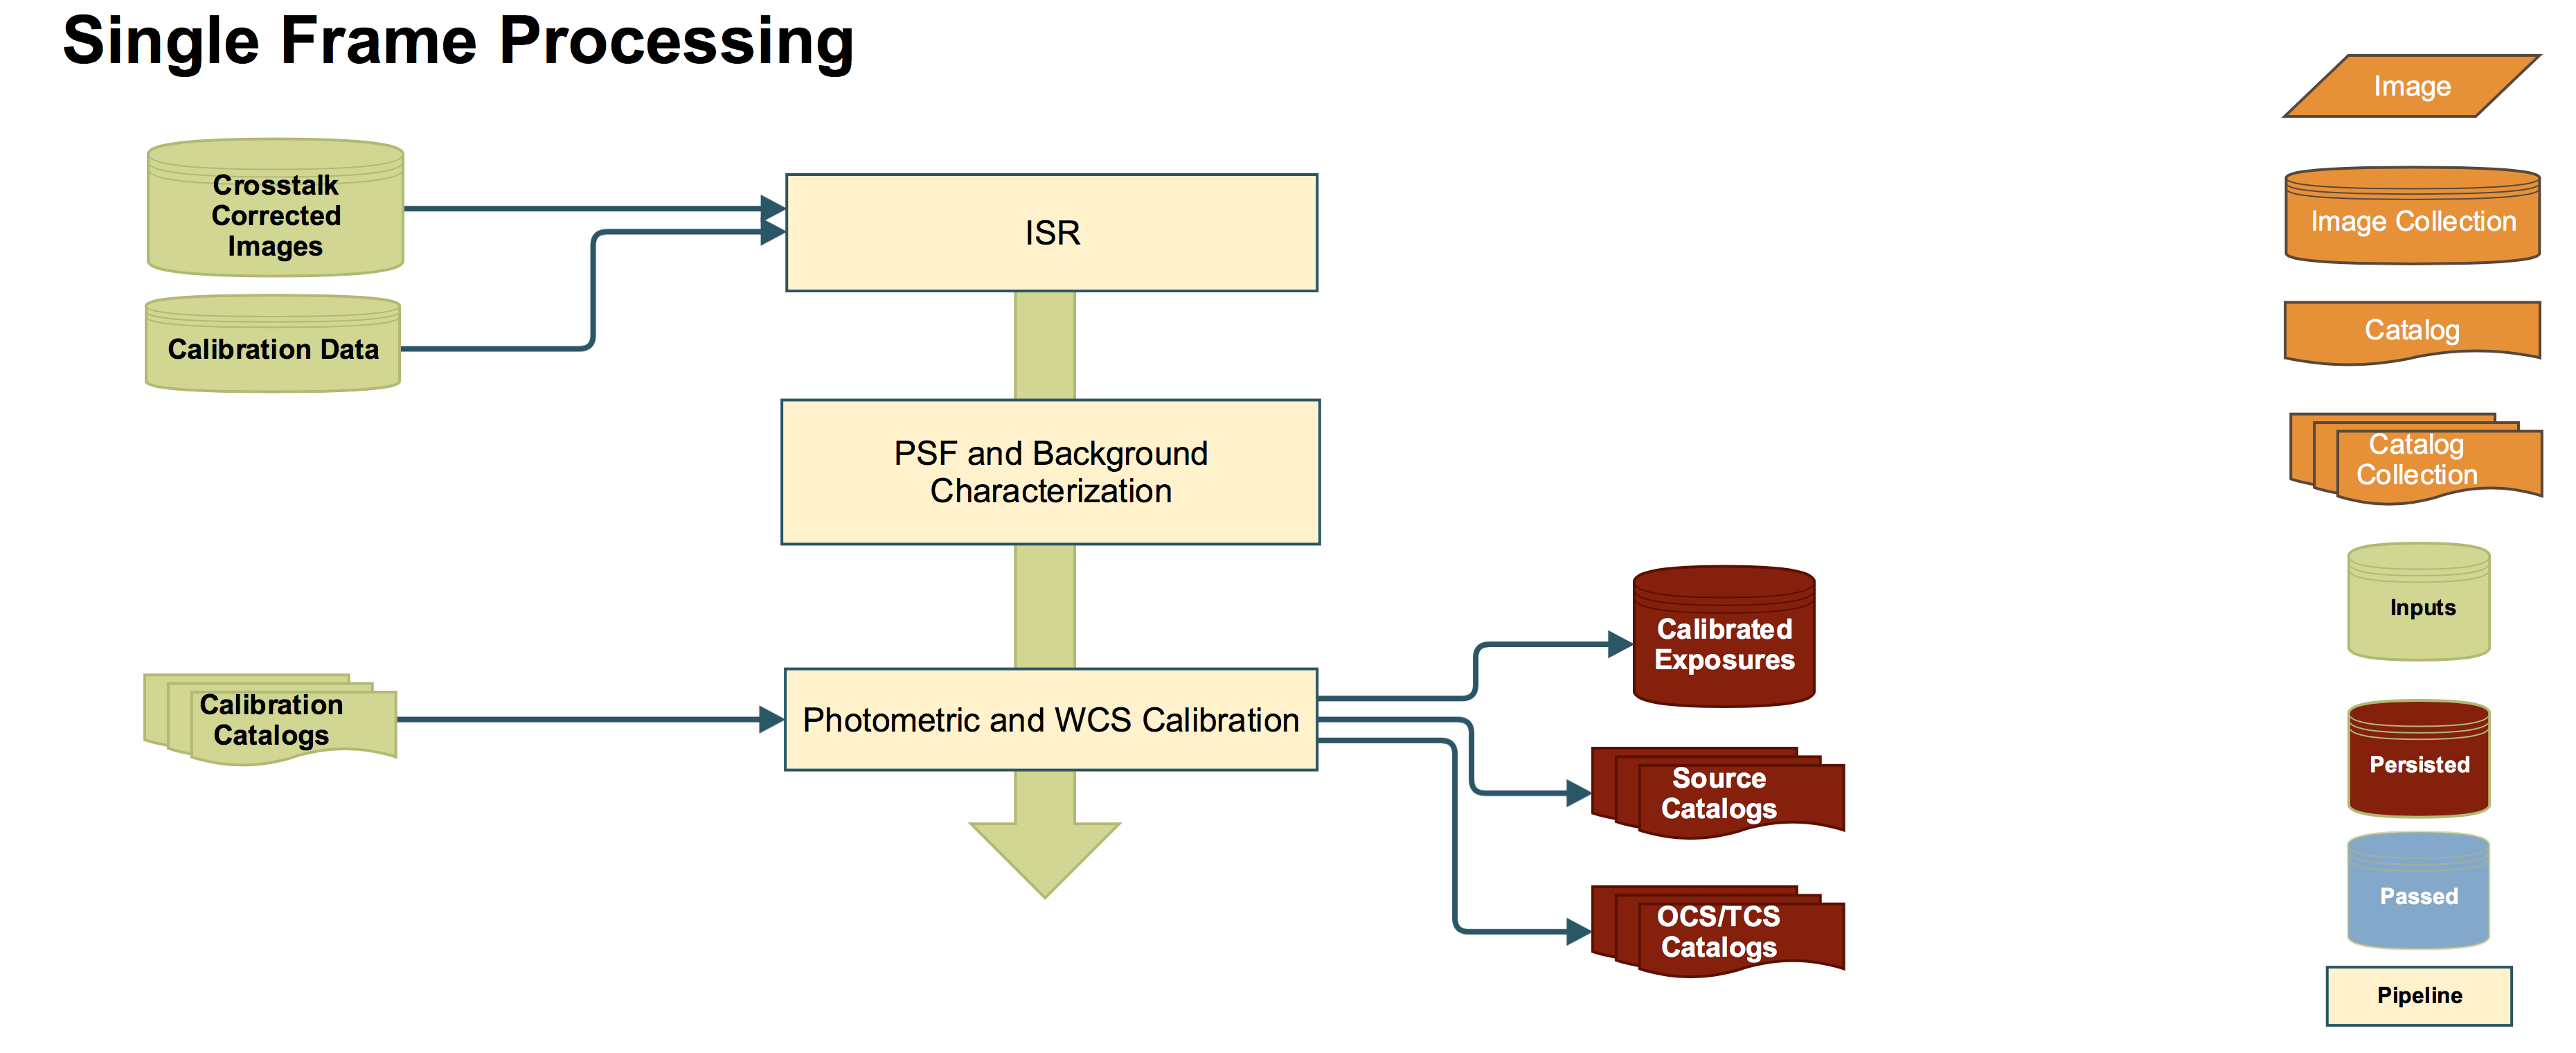
\includegraphics[width=0.9\textwidth]{figures/SFM.png}
\caption{\label{fig:apSFM} Single frame processing of the nightly data: instrument signature removal, astrometric and photometric calibration, background and PSF estimation from the cross-talk corrected camera images.}
\end{center}
\end{figure}

%SFM pipeline functions include:
%\begin{itemize}
%\item Assembly of per-amplifier images to an image of the entire CCD;
%\item Instrumental Signature Removal;
%\item Cosmic ray rejection and snap combining;
%\item Per-CCD determination of zeropoint and aperture corrections;
%\item Per-CCD PSF determination;
%\item Per-CCD WCS determination and astrometric registration of images;
%\item Per-CCD sky background determination;
%\item Source detection and measurement on single frame images
%\item Generation of metadata required by the OCS
%\end{itemize}

\subsubsection{Input Data}
\label{sec:apSFMinput}

\paragraph*{Raw Camera Images:} Amplifier images that have been corrected for crosstalk and bias by the camera software. All images from a visit should be available to the task (including snaps). An approximate WCS is assumed to be available as metadata derived from the Telescope Control System with an absolute pointing uncertainty (for a full focal plane) of 2 arcseconds (OSS-REQ-0298) and the field rotation known to an accuracy of 32 arcseconds (LTS-206).
%\begin{note} question into Steve R about Camera operations - DM to provide request for operations on images that camera team will undertake \end{note}

\paragraph*{Reference Database:} A full-sky astrometric and photometric reference catalog of stars derived either from an external dataset (e.g.\ Gaia) or from the Data Release Processing. Given the current Gaia data release timeline the initial reference catalog is expected to have an astrometric uncertainty of $<0.5$ milliarcseconds and a photometric uncertainty of $<$20 millimag (for a $V=19$ G2V star). The expected release of these calibration catalogs is 2018 and will be derived from the Gaia spectrophotometric observations of non-variable sources.

\paragraph*{Calibration Images:} Flat-field calibration images for all passbands and all CCDs appropriate for the time at which the observations were undertaken. No corrections will be made in the flat-fields for non-uniform pixel sizes - the flat-fields will correct to a common  surface brightness. A flat SED will be assumed for all flat field corrections. Fringe frame calibration images scaled to an amplitude derived from the sky background (i.e.\ no sky spectrum will be available).

\paragraph*{Image Metadata:} List of the positions and extents of CCD defects for all CCDs within the focal plane; electronic parameters for all CCDs (saturation limits, readnoise parameters), electronic and physical footprint for the CCDs, linearity functions, models for the variation in the PSF width with source brightness (brighter-fatter), and parameterized models for a component-based  WCS (e.g.\ a series of optical distortion models) as needed.

\subsubsection{Output Data}
\label{sec:apSFMoutput}

\paragraph*{CalExp Images:} A calibrated exposure (CalExp) is an \hyperref[sec:spImagesExposure]{Exposure} object. The CalExp contains the image pixel values, a variance image, a bitwise mask, a representation of the PSF, the WCS (possibly decomposed into separable components), a photometric calibration object, and a model for the  background. For the alert production, it is not anticipated that a model of the per-pixel covariance will be persisted but this will be revisited dependent on the performance of image subtraction and anomaly characterization as described in \ref{sec:apAlertGeneration}.

\paragraph*{Source Databases:} A catalog of \Sources with measured features described in \ref{sec:apSourcemeasurement}.

\paragraph*{OCS Database} A parameterization of the PSF, WCS, photometric zeropoint, and depth for each CCD in a visit. The PSF may be a simplified version (e.g.\ a single Gaussian) of that derived for the Alert production. These data will be made available to the Telescope Control System (TCS) to assess the success of each observation. A limited version of nightly SFM could be run on the summit to generate this information or the  data will be persisted within a database at the data center that will be accessible to the TCS.


\subsubsection{Instrumental Signature Removal}
\label{sec:apISR}
Instrumental Signature Removal characterizes, corrects, interpolates and flags the camera (or raw) amplifier images to generate a flat-fielded and corrected full CCD exposure.

\paragraph{Pipeline Tasks}
\begin{itemize}
\item Mask the image defects at the amplifier level based on the CCD defect lists, and the per CCD saturation limits
\item Assemble the amplifiers into a single frame (masking missing amplifiers)
\item Apply full frame corrections: dark current correction, flat field to preserve surface brightness, fringe corrections. Flat fields will assume a flat spectral energy distribution (SED) for the source. Fringe frames will be normalized by fitting to the observed sky background.
\item Apply pixel level corrections: apply a correction model for brighter-fatter to homogenize the PSF, correct for static pixel size effects based on a model
\item Interpolate across defects and saturated pixels assuming a model for the PSF (with a nominal FWHM). An estimate of the PSF will be needed for this operation (from the TCS/OCS) or interpolation may be needed to be performed at the end of \ref{sec:apPSFBackground}.
\item Apply a cosmic ray detection algorithm as described in \ref{sec:acCosmicRayDetection}
\item Generate a summed and difference image from the individual snaps propagating the union of the mask pixels in each snap
\end{itemize}

Dependent on the properties of the delivered LSST image quality for 15 second snaps it may be required to model any bulk motion between snaps prior to combination (e.g.\ if dome seeing or the ground layer dominate the lower order components of the seeing).

\subsubsection{PSF and background determination}
\label{sec:apPSFBackground}

Given exposures that have been processed through Instrument Signature Removal, \Sources must be detected to determine the astrometric and photometric calibration of the images. As noted previously an iterative procedure will be adopted to generate an estimate of the background and PSF, and to characterize the properties of the detected sources.  Convergence criteria for this procedure are not currently defined. The default implementation assumes three iterations.

\paragraph{Pipeline Tasks}

The iterative process for PSF and background estimation comprises,
\begin{itemize}
\item Background estimation on the scale of a single CCD is as described in \ref{sec:acBackgroundEstimation}, which divides the CCD into subregions and estimates the background using a robust mean from non-source pixels.
\item Subtraction of the background and the detection of sources as described in \ref{sec:acSourceDetection}. The initial detection threshold for source detection will be 5$\sigma$, with $\sigma$ estimated from variance image plane.
\item Measurement of the properties of the detected sources (see \ref{sec:apSourcemeasurement}). Dependent on the density of sources it may be necessary to deblend the images as described in \ref{sec:acDeblending}
\item Selection of isolated PSF candidate stars based on a signal-to-noise threshold (default 50 $\sigma$). This threshold is significantly deeper than the magnitude limit for Gaia astrometric catalogs but is the threshold at which the astrometric error on the centroid due to photon noise is less than 10 mas and the photometric noise is less than 2\% for the case of the use of a deeper DRP derived reference catalog.
\item Single CCD PSF determination using the techniques described in \ref{sec:acSingleCCDPSF} and the selected bright sources
\item Masking of source pixels within the CCD (growing the footprint of the \Sources to mask the outer regions of the \Source profiles will likely be required to exclude contributes to the background from low surface brightness features).
%\item Single CCD \hyperref[sec:acModelSpatialPSF]{PSF spatial model}
\end{itemize}

The default expectation is that all tasks within this procedure would iterate until convergence.  There maybe significant speed optimizations to be gained by excluding the \Source detection step after an initial detection if the number of sources does not change significantly with updates to the background model.
%\begin{note} Treatment of covariance \end{note}

\subsubsection{Source measurement}
\label{sec:apSourcemeasurement}

For the \Source catalog generated in \ref{sec:apPSFBackground}, source properties are measured using a subset of features described in \ref{sec:acMeasurement}. Source measurement is for all sources within the \Source catalog and not just the bright subset used to calibrate the PSF.  We anticipate using the following plugin algorithms within the \Source measurement step,
\begin{itemize}
\item Centroids based on a static PSF model fit (see \ref{sec:acCentroidAlgorithms} and \ref{sec:acStaticPointSourceModels})
\item Aggregation of pixel flags as described in \ref{sec:acPixelFlags}
\item Aperture Photometry as geven in \ref{sec:acAperturePhotometry} (but only for one or two radii)
\item PSF photometry given in \ref{sec:acStaticPointSourceModels} assuming a static PSF model fit
\item  An aperture correction estimated assuming a static PSF model and measurement of the curve of growth for  detected sources as given in \ref{sec:acApCorr}
\end{itemize}
%\begin{note} why only one or two radii \end{note}

\subsubsection{Photometric and Astrometric calibration}

Photometric and astrometric calibration entails a ``semi-blind'' cross match (because the pointing of the telescope is known to an accuracy of 2 arcseconds) of a reference catalog derived either from the DRP \Objects or from an external catalog (see \ref{sec:apSFMinput}), the generation of a WCS (on the scale of a CCD or full focal plane), and the generation of a photometric zeropoint (on the scale of a CCD). These algorithms must degrade gracefully for the case of larger pointing errors (e.g.\ during the initial calibration of the system during commissioning) and may need to operate in a ``blind'' mode where the pointing and orientation of the telescope is not known.

\paragraph{Pipeline Tasks}

The photometric and astrometric calibration is expected to be performed at the scale of a single CCD. It is possible that the calibration process will need to be extended to larger scales (up to a full focal plane) if there is significant structure in the photometric zero point, or if astrometric distortions cannot be calibrated at the scale of the CCD with sufficient accuracy (i.e.\ the astrometric distortions do not dominate the false positives in the image subtraction). A full focal plane level calibration strategy will introduce synchronization points within the processing of the CCDs as the detections on all CCDs will need to be aggregated prior to the astrometric fit.

The procedures used to match and calibrate the data are,
\begin{itemize}
\item CCD level source association between the DRP reference catalog (or external catalog) and \Sources detected during the PSF and background estimation stage will use a simplified Optimistic B approach described in \ref{sec:acSingleCCDReferenceMatching}. Given an astrometric accuracy of $<0.5$ milliarcseconds from external catalogs such as Gaia (for a $V=19$ G2V star) or  an accuracy of $<50$ milliarcseconds for the DRP catalogs the search radii for sources will be dominated by the uncertainties in the pointing of the telescope and the rotation angle of the camera.
\item Generation of a photometric solution on the scale of a single CCD as described in \ref{sec:acSingleCCDPhotometricFit}
\item Fitting of a WCS astrometric model for a single CCD  using the algorithms given in \ref{sec:acSingleCCDAstrometricFit}. The WCS model is expected to be composed of a sum of transforms or astrometric components (e.g.\ a optical model for the telescope, a lookup table or model for sensor effects such as tree rings).
\item Persistance of the astrometric, PSF, and photometric solutions for possible use by the Telescope Control system (TCS) (see \ref{sec:apSFMoutput})
\end{itemize}

Given the number of stars available on a CCD or the complexity of the astrometric solutions for the LSST (e.g.\ the decomposition of the WCS into components) it may be necessary that the astrometric and photometric solutions be performed for a full focal plane and not just a CCD.  For these cases the algorithms used will be single visit matching (see \ref{sec:acSingleVisitReferenceMatching}),  single visit photometric solutions (see \ref{sec:acSingleCCDPhotometricFit}), and single visit astrometric fits (see \ref{sec:acSingleVisitAstrometricFit}). Fitting to a full focal plane introduces a synchronization point in the alert processing where all CCDs must have completed their previous processing steps prior to the astrometric calibration.

Astrometric and photometric solutions  within crowded fields will utilize the bright and easily isolated sources within a CCD image. The order of the WCS used in the astrometric fits will, therefore, depend on the number of calibration \Sources that are available.

\subsection{Alert Generation Pipeline (\wbsDiffim)}
\label{sec:apAlertGeneration}

The Alert Generation pipeline identifies variable, moving, and transient sources within a calibrated exposure by subtracting a deeper template image (see Figure~\ref{fig:apAlertgen}). The \DIASources detected on a DiffExp are associated with known \DIAObjects and \SSObjects (that have been propagated to the date of the CalExp exposure) and their properties measured. The process for image differencing requires the creation or retrieval of a TemplateCoadd, the matching of the  astrometry and PSF of the TemplateCoadd to a CalExp, and subtracting the template image from the CalExp. Spurious \DIASources will be removed using morphological and environment based classification algorithms.

The Alert Generation pipeline is required to difference, and detect and characterize \DIASource sources within 24s (allowing for multiple cores and multithreading of the processing).
%The requirement on the algorithms for purity and completeness of the sample is given by the \DMSR\@. Image differencing shall perform as well in crowded as in uncrowded fields.


\begin{figure}[th]
\begin{center}
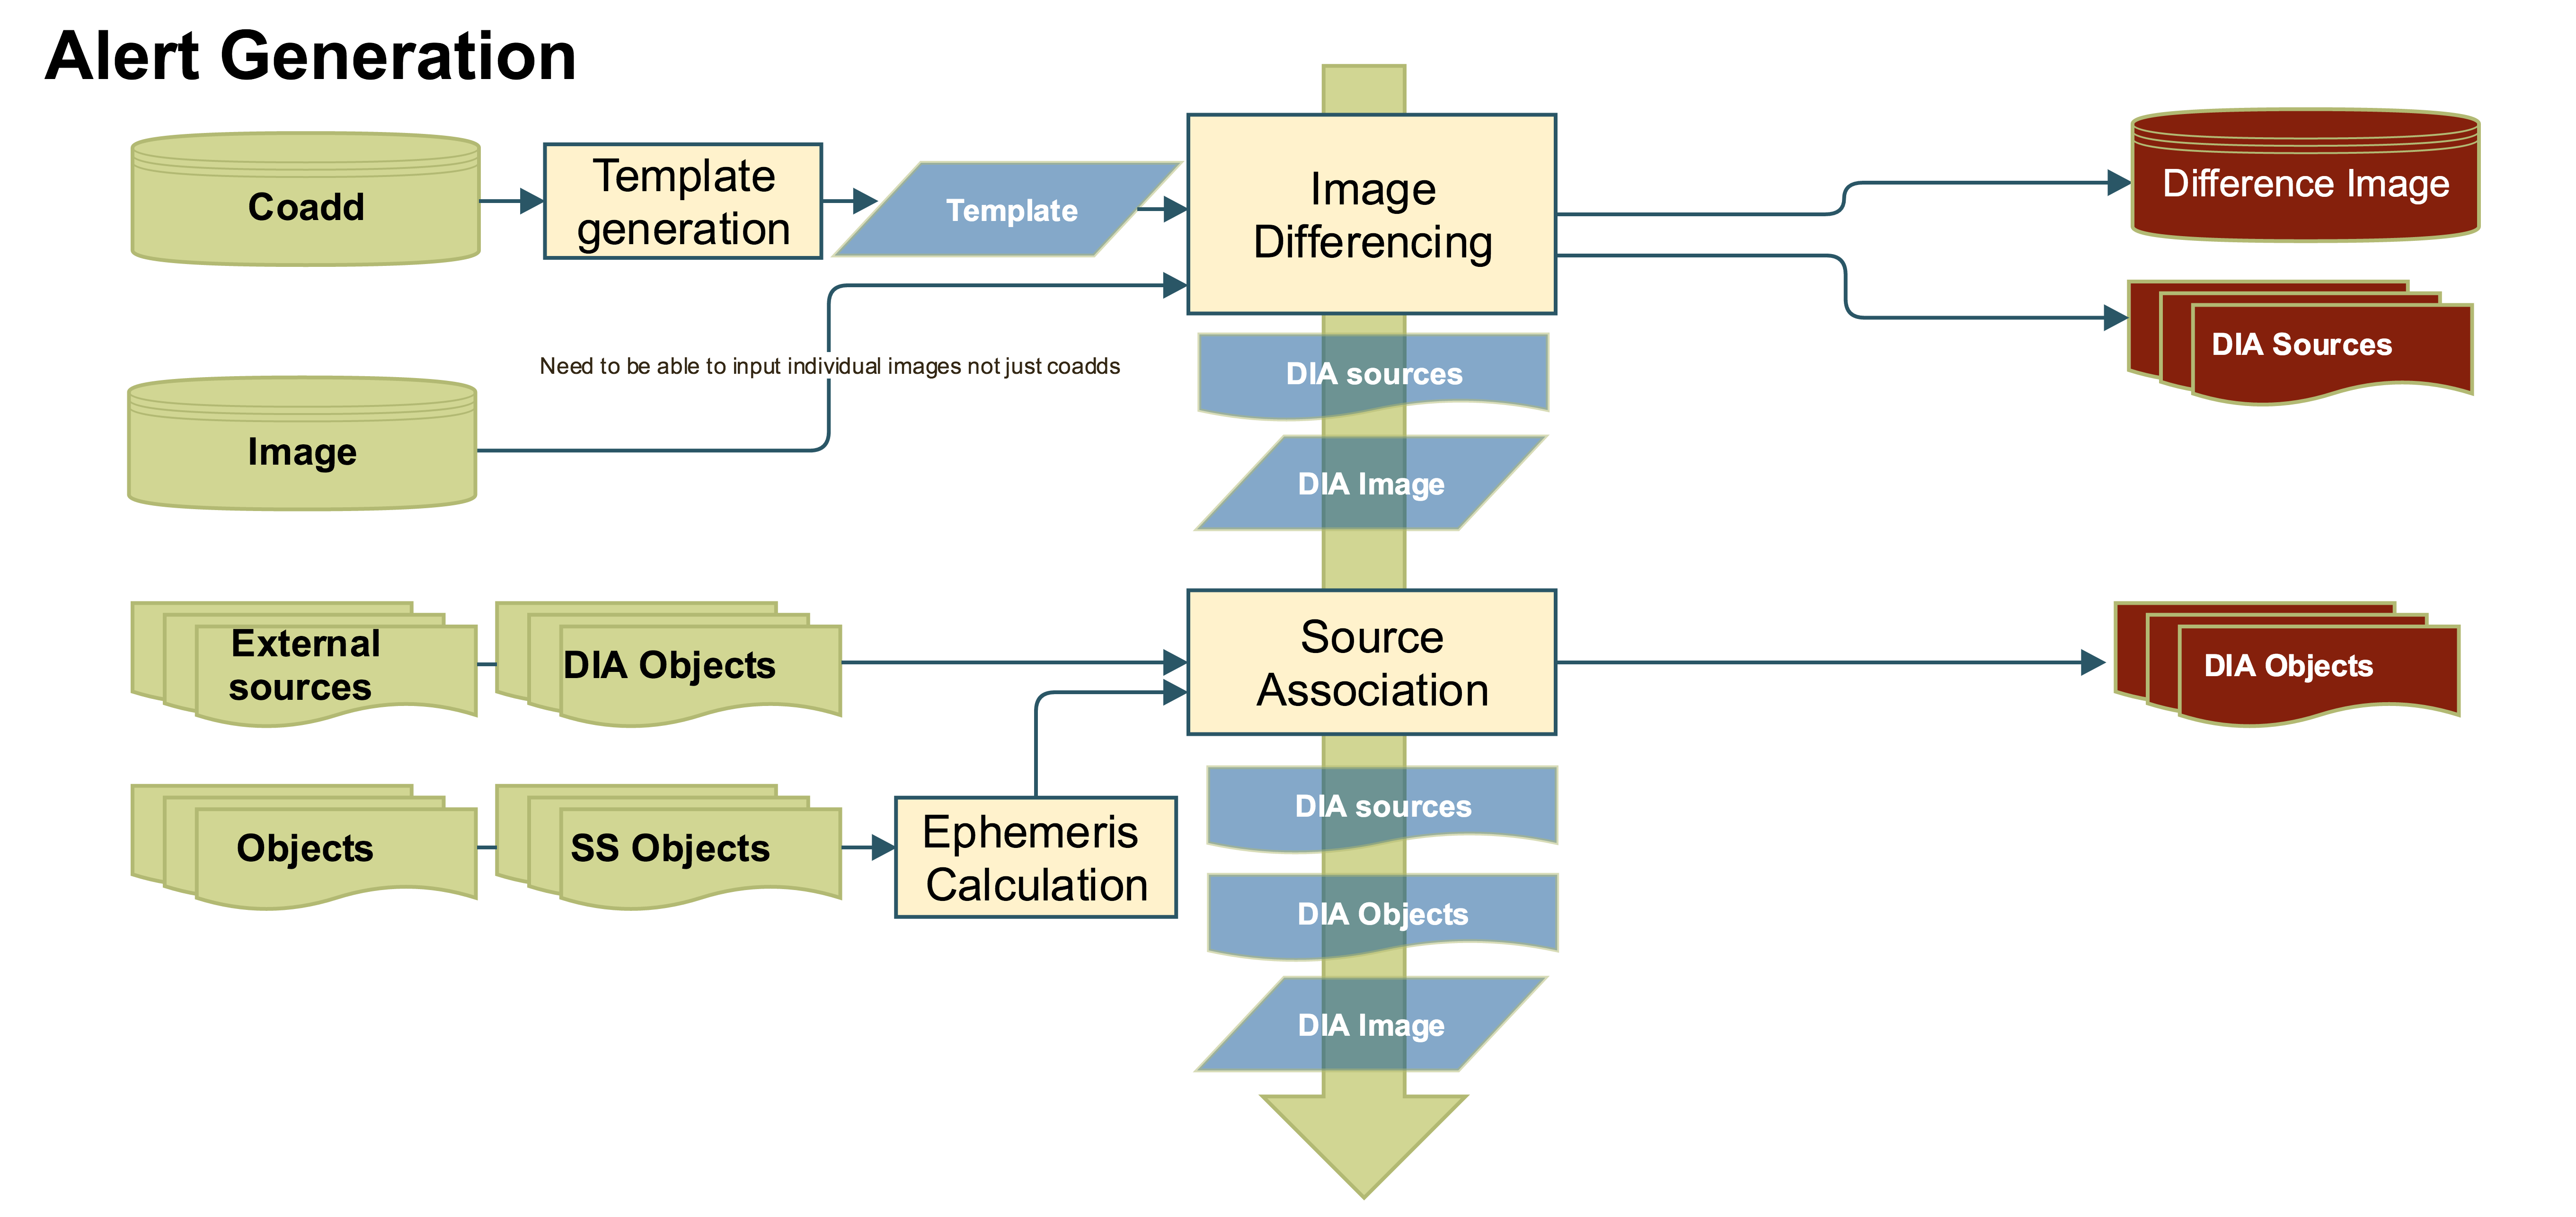
\includegraphics[width=0.9\textwidth]{figures/Alert_Generation.png}
\caption{\label{fig:apAlertgen} Generation of alerts from the nightly data: image differencing and measurement of the properties of the \DIASources, identification and filtering of spurious events, association of previously detected \DIAObjects and \SSObjects with the newly detected \DIASources. }
\end{center}
\end{figure}
\subsubsection{Input Data}
\label{sec:apAGInput}

\paragraph*{CalExp Images:} Calibrated exposure processed through \ref{sec:apSingleFrameProcessing} with associated WCS, PSF, mask, variance, and background estimation.

\paragraph*{Coadd Images:} TemplateCoadd images that spatially overlap with the CalExp images processed through \ref{sec:apSingleFrameProcessing}. This coadded image is optimized for image subtraction and is expected to be characterized in terms of a tract/patch/filter. Generation of this template may account for differential chromatic refraction or be generated for a limited range of airmass, seeing, and parallactic angles.

\paragraph*{Object Databases:} \Objects that spatially overlap with the CalExp images processed through \ref{sec:apSingleFrameProcessing}. This \Object catalog will provide the source list for determining nearest neighbors to the detected \DIASources.


\paragraph*{DIAObject Databases:} \DIAObjects that spatially overlap with the CalExp images processed through \ref{sec:apSingleFrameProcessing}. This \DIAObject catalog will provide the association  list against which the \DIASources will be matched.

\paragraph*{SSObject Databases:} The \SSObject list at the time of the observation. The \SSObject positions will be propagated to the date of the CalExp observations and will provide an association  list for cross-matching against the detected \DIASources to identify known Solar System objects.

\paragraph*{Reference classification catalogs:} Classification of \DIASources based on their morphological features (and possibly estimates of the local density or  environment associated with the \DIASource) will be undertaken prior to association in order to reduce the number of false positives. The data structures that define these classifications will be required as an input to this spuriousness analysis.



\subsubsection{Output Data}
\label{sec:apAGOutput}

\paragraph*{DiffExp Images:} Image differences derived by subtracting a TemplateCoadd from a CalExp image.

\paragraph*{DIASource Databases:} \DIASources detected and measured from the DiffExps using the set of parameters described in Table~\ref{table:ap_features} will be persisted.


\paragraph*{DIAObject Databases:} \DIASource will be associated with existing \DIAObjects and persisted. New \DIASource (i.e.\ those not associated) will generate a new instance of a \DIAObject.


\subsubsection{Template Generation}
\label{sec:apCRTemplates}

Template generation requires the creation or retrieval (see \ref{sec:acRetrieveTemplate}) of a TemplateCoadd that is matched to the position and spatial extent of the input CalExp. Generation of the TemplateCoadd could be from a persisted Coadd that was generated from CalExp exposures with comparable (within a predefined tolerance) airmass and parallactic angles, or from a model that corrects for the effect of  differential chromatic refraction (see \ref{sec:acDCRTemplates}). It is expected that these operations would be undertaken on a CCD level but for efficiency the TemplateCoadd might be returned for a full focal plane or a series of \textit{patches}  or a \textit{tract}.


\paragraph{Pipeline Tasks}

\begin{itemize}
\item Query for a TemplateCoadd images that are within a given time interval of the CalExp  (default 2 years) of the current CCD image, and are within a specified airmass and parallactic angle.
\item (optional) Derive a seeing and DCR corrected TemplateCoadd from a model (see DCR template generation in \ref{sec:acDCRTemplates}). The current prototype approach assumes that the TemplateCoadd  will be derived for the zenith and will comprise a data cube with spatial and wavelength dimensions (a low resolution spectrum per pixel). Propagating to the observation will require aligning the DCR correction in the direction of the parallactic angle of the CalExp.
\end{itemize}

\subsubsection{Image differencing}

Image differencing incorporates the matching of a TemplateCoadd to a CalExp (astrometricly and in terms of image quality), subtraction of the template image, detection and measurement of \DIASources, removal of spurious \DIASources, and association of the \DIASources with previously identified \DIAObjects, and \SSObjects.

\paragraph{Pipeline Tasks}

\begin{itemize}
\item Determine a relative astrometric solution from the WCS of the TemplateCoadd image and CalExp image
\item Match the DRP \Sources for the TemplateCoadd (see \ref{sec:drpFinalImChar}) against \Sources from the SFM pipeline (see \ref{sec:apSingleFrameProcessing}) of the raw images.
\item Warp or resample the TemplateCoadd using a Lanczos filter  (as described in \ref{sec:spWarp}) to match the astrometry of the CalExp. It is possible that astrometricly matching the TemplateCoadd and CalExp using faint source will need to be undertaken dependent on the accuracy of the WCS.
\item For CalExp images with an image quality that is better than the TemplateCoadd preconvolve the CalExp image with the PSF. Use a  convolution kernel (see \ref{sec:spKernels}) that is matched to the source detection kernel. This reduces the need for deconvolution in the PSF matching (see \ref{sec:acImageSubtraction})
\item Match the PSF of the CalExp and TemplateCoadd images as described in \ref{sec:acDiffImDecorrelation} and construct a spatial model for the matching kernel. This approach may include matching to a common PSF through homogenization of the PSF (see \ref{sec:acPSFHomogenization}.
\item Apply the matching kernel to the TempCoadd and subtract the images to generate a DiffExp (as described in \ref{sec:acImageSubtraction}). Dependent on the relative signal-to-noise in the science and template image decorrelation of the template image due to the convolution of the template with a matching kernel may be necessary (see \ref{sec:acDiffImDecorrelation})
\item Detect \DIASources on the DiffExp using the algorithms described in \ref{sec:acSourceDetection}. Convolution with a detection kernel will depend on whether the CalExp was preconvolved in item 4.
\item Measurements of the \DIASources on the DiffExp will include dipole models and trailed PSF models (see  \ref{sec:acDipoleModels} and \ref{sec:acTrailedPointSourceModels} and parameters described in Table~2 of the \DPDD . The specific algorithms used for measurement of \DIASources will depend on whether the CalExp image was preconvolved.
\item Measurement of the PSF flux on snap difference images for all \DIASources.
\item The application of spuriousness algorithms, also known as ``real-bogus'', may be applied at this time dependent on whether the number of false positives is less than 50\% of the detected sources (see \ref{sec:acSpuriousnessAlgorithms})\footnote{The requirement for a 50\% false positive rate is given in the XXX and impacts the sizing model for the alert stream}. \DIASources classified as spurious at this stage may not be persisted (dependent on the density of the false positives). The default technique will be based on a trained random forest classifier. It is likely that the training of this classifier will need to be conditioned on the image quality and airmass of the observations.
\end{itemize}

\subsubsection{Source Association}
\label{sec:apSourceAssoc}

In Source Association \DIASources detected within a given CCD will be cross-matched or associated (see \ref{sec:acDIAObjectGeneration}) with the \DIAObject table and the \SSObjects (whose ephemerides have been generated for the time of the current observation). The association will be probabilistic  and account for the uncertainties within the positions. The association may include flux and priors on expected proper motions for the sources. External targets (e.g.\ well localized transient events from other telescopes or instruments) can be incorporated within this component of the nightly pipeline (essentially treating external sources as additional \DIAObjects and associating them with the \DIASources) enabling either matching to \DIASources or generation of forced photometry at the position of the external source.

\paragraph{Pipeline Tasks}

\begin{itemize}
\item Generate the positions of \SSObjects that overlap a DiffExp given its observation time by propagating the \SSObject orbit (see \ref{sec:acEphemerisCalculation})
\item As described in \ref{sec:acDIAObjectGeneration} source association will be undertaken for all \DIASources. Matching will be to \DIAObjects, and the ephemerides of \SSObjects. Positions for \DIAObjects will be based on a a time windowed (default 30 day) average of the \DIASources that make up the \DIAObject. A linear motion model for parallax and proper motion will be applied to propagate the \DIAObject to the time of the observation. A probabilistic association may need to account for one-to-many and many-to-one associations.  In dense regions it may be necessary to generate joint associations across all \DIAObjects (and associated \DIASources) in the local  vicinity of a \DIASource to correct for mis-assignment from previous observations. This could include the pruning and reassignment of \DIASources between \DIAObjects. A baseline approach for nightly processing will be to select based on a maximum a posteriori estimate for the association.
\item \DIASources will be positionally matched to the nearest 3 stars and 3 galaxies in the DRP \Object database. In its simplest case the search algorithm will be a tree-based nearest neighbor search (the default radius for association is not defined) . The matched \Objects will be persisted as a measure of local environment.
\item \DIASources unassociated with a \DIAObject will instantiate a new \DIAObject.
\item The aggregate positions for the \DIAObjects will be updated based on a rolling time window (default 30 days).
\item Proper motion and parallax of the \DIAObject will be updated using a linear model as described in \ref{sec:acStellarMotionFitting}.
%It is not currently clear if there is a science case for generating proper motions and parallaxes within the %DIAObjects if the DRP Objects are available for each source.
\end{itemize}


\clearpage

\subsection{Alert Distribution Pipeline (\wbsAP)}

The Alert Distribution Pipeline takes the newly discovered \DIAObjects (including their associated historical observations) and all related metadata as described in the \DPDD, and delivers alert packets in \VOEvent format to a variety of endpoints via standard IVOA protocols (eg., \VOEvent Transport Protocol; VTP\@). Packaging of the event will include the generation of postage stamp cutouts (30x30 pixels on average) for the difference image and the template image together with the variance and mask pixels for these cutouts.

On average, each LSST visit will result in $\sim 2M$ alerts per night. This number includes both real and spurious detections and will be highly dependent on where we look on the sky. Because of this, the \SRD requires that the design of the LSST alert system should be able to handle 10$^7$ events per night, which corresponds to 10$^4$ alerts per visit or 50 alerts per CCD (with each visit lasting 39 seconds). All alerts should be transmitted within 60s of the closure of the shutter of the final snap within a visit.

For a nightly event rate of 10$^7$, and assuming the schema described in Tables 1 and 2 in the \DPDD together with the generation of the postage stamp cutouts, the compressed \VOEvents data stream amounts to approximately 600GB of data per night (assuming no filtering of the data).  The Alert Distribution pipeline is designed to distribute these alerts with a workflow, including the access point of external event brokers, shown in Figure~\ref{fig:apAlertDistribution}.

In addition to the full data stream the Alert Generation Pipeline will provide a basic alert filtering service. This service will run at the LSST U.S. Archive Center (at NCSA). It will enable astronomers to create filters (see  \ref{sec:apQueue}) that limit what alerts, and what fields from those alerts, are ultimately forwarded to them. These \emph{user defined filters} will be configurable with a simplified SQL-like declarative language. Access to this filtering service will require authentication by a user.

\VOEvent alerts will be persisted in an alert database as well as distributed through a message queue. The alert database (AlertDB) will be synchronized at least once every 24 hours and will be queriable by external users. The message queue that distributes the alerts is expected to have the capability  to replay events for the case of a break in the network connection between the queue and client but not to support general queries.

\begin{figure}[th]
\begin{center}
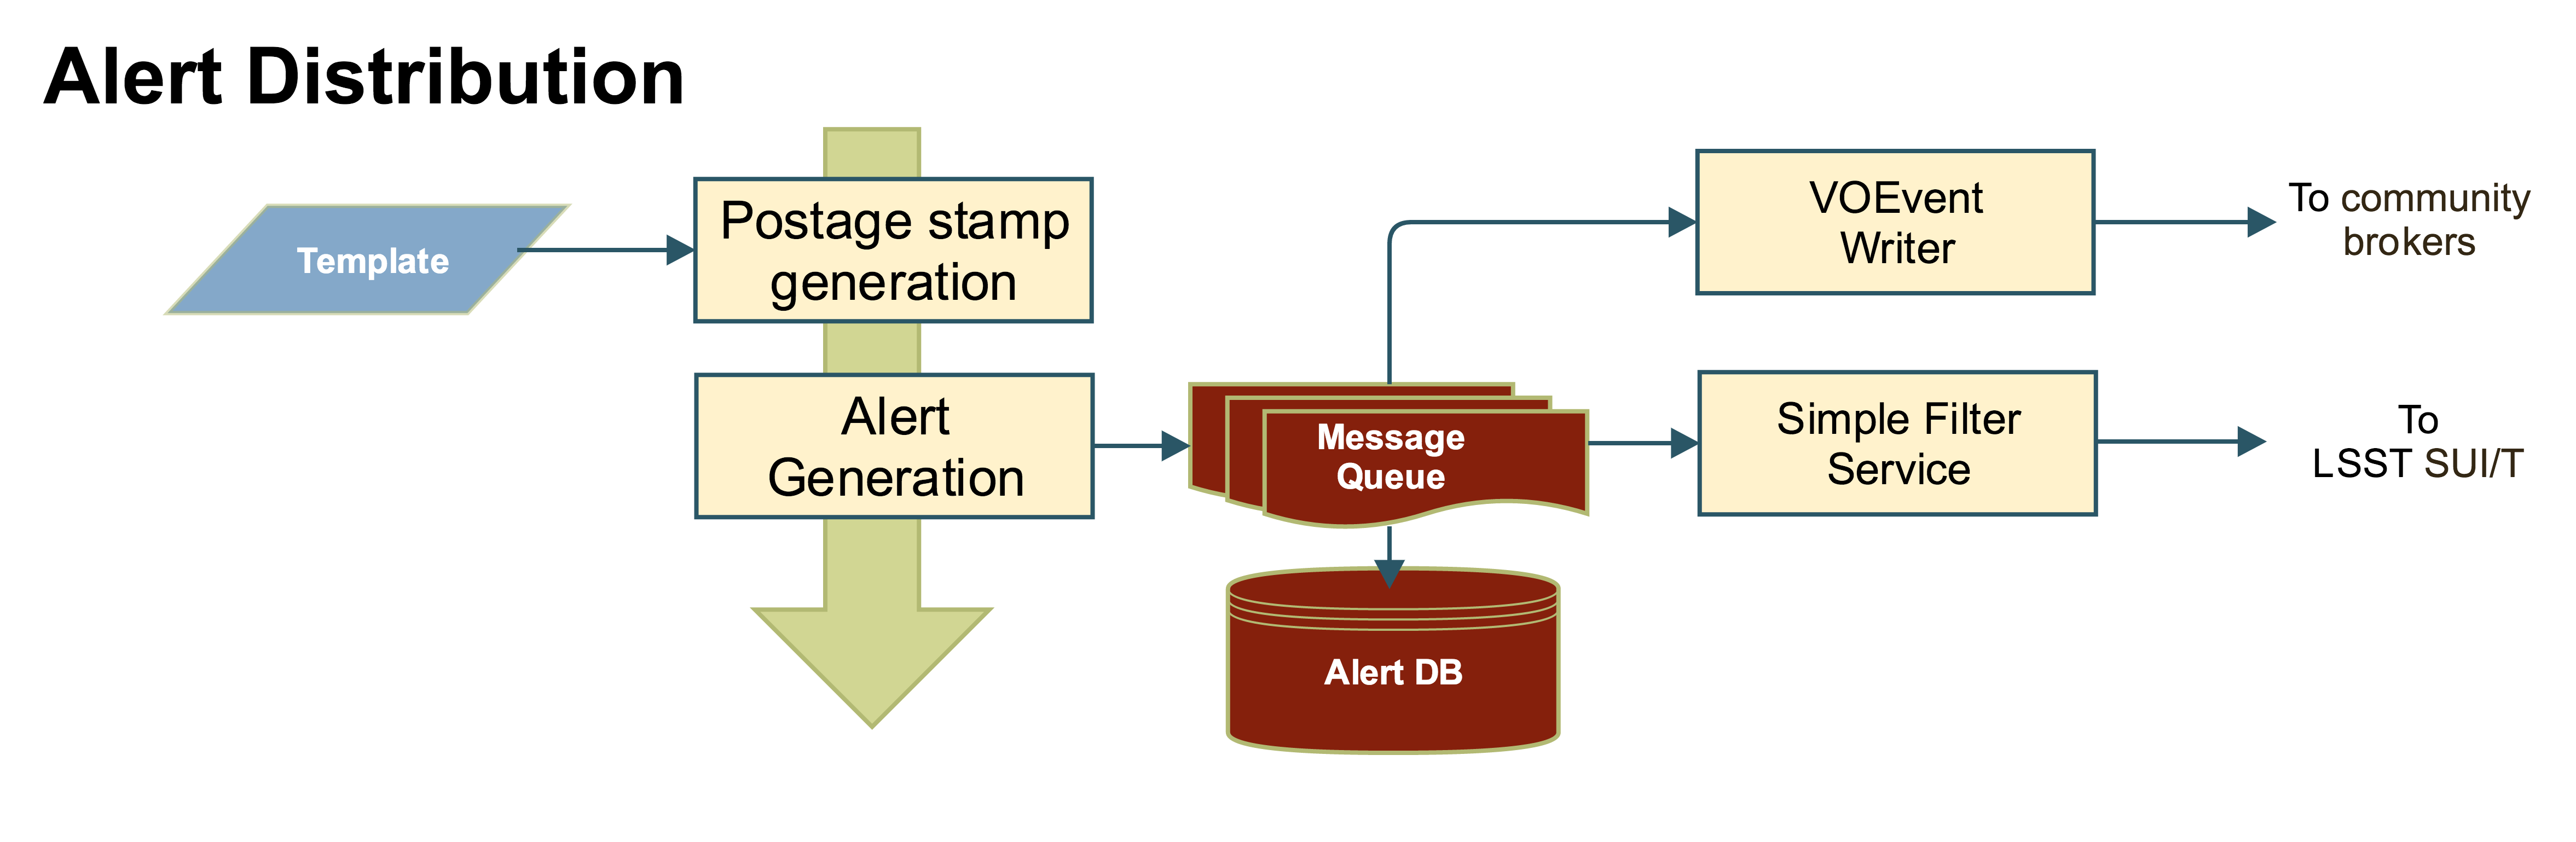
\includegraphics[width=0.9\textwidth]{figures/Alert_Distribution.png}
\caption{\label{fig:apAlertDistribution} Distribution of alerts from the nightly processing: generation of postage stamps around each detected \DIASource, distribution of the \DIAObjects as VOEvents, simple filtering of the event stream, and persistence of the events in a database.}
\end{center}
\end{figure}

\subsubsection{Input Data}
\label{sec:apADInput}

\paragraph*{DIAObject Database:} \DIAObjects, with new \DIASources, generated through image differencing will be used to create alert packets.

\paragraph*{Difference Images:} The DiffExp will be used to  generate postage stamp (cut-out) images of \DIASources within the CCD.

\paragraph*{Coadd Images:} The TemplateCoadd used in image subtraction will be used to  generate postage stamp images of the template image for \DIAObjects.


\subsubsection{Output Data}

\paragraph*{\VOEvent Database:} \VOEvents generated from the \DIAObjects and cutouts will be persisted within a database (e.g.\ a noSQL database) or object store.




\subsubsection{Alert postage stamp generation}

Creates the associated image cutouts (30x30 pixels on average) for all detect \DIAObjects (cutouts are generated from the current observation and not from historical observations).

\paragraph{Pipeline Tasks}

 \begin{itemize}
\item Extract from the DiffExp the cutout of each \DIAObject with a \DIASource detected within the current observation.  Cutout images will be scaled to the size of the \DIASource but on average will be 30x30 pixels. Variance and mask planes, WCS, background model, and associated metadata will be persisted. The prototype implementation assumes that these cutouts will be persisted as FITS images with a projection that is the  native projection of the DiffExps.

\item Extract from the TemplateCoadd  a cutout of each \DIAObject with a \DIASource detected within the current observation.  Cutout images will be identical in size and footprint as those derived from the DiffExp. Variance and mask planes, WCS, and associated metadata will be extracted with the pixel data. The prototype implementation assumes that these cutouts will be persisted as FITS imagesand that the projection will be that of  the DiffExps.
\end{itemize}

\subsubsection{Alert queuing and persistance}
\label{sec:apQueue}

The alert queue  distributes and persists \DIAObject with new \DIASources as \VOEvents through a message queue. It includes a \textit{limited} filtering interface but persists the full \VOEvents in an AlertDB. The event message stream and the AlertDB will be  synchronized at least once every 24 hours.


\paragraph{Pipeline Tasks}

\begin{itemize}
\item Publish \DIAObjects to a caching message queue (e.g.\ \hyperref[http://kafka.apache.org]{Apache Kafka}) through the butler. The prototype implementation assumes a distributed and partitioned messaging system that uses a \hyperref[https://en.wikipedia.org/wiki/Publish_subscribe_pattern]{publication-subscription} model for communication between clients and the queue. This model maintains feeds of messages in categories called topics. An example topic would be a \DIAObject. Whether a topic would comprise a full \DIAObject or a subset of the data remains open (passing subsets of parameters as individual topics would require that the client be able to synchronize and join topics into a full \DIAObject). For each of the 189 CCDs, approximately 50 events will be passed as messages to the messaging queuing system. The distribution of the events from a given CCD will not be synchronized with other CCDs within the focal plane (alerts from each CCD will be independently processed).

\item A consumer layer will subscribe to the  message queue and package them as \VOEvents and distribute these events to external users. To allow for network outages between the message queue and the consumer the message queue must be able to replay previous events.
\item  The consumer layer will provide a command line API to define simple queries or filters of the events (limited to querying on existing \DIAObject fields, or filtering the attributes of the \DIAObject). Web-based interfaces to the consumer layer will be developed by SUIT.
\item Filtered or the full stream of \DIAObjects will be packaged into \VOEvents and broadcast to VOEvent clients through the consumer layer
\item A full, unfiltered, VOEvent alert stream will be broadcast to the AlertDB using the consumer layer.
\item Prior to the start of the subsequent night's observations, the message queue will be flushed and synchronized with the AlertDB. It is possible to persist the message queue on longer timescale but it is a requirement hat synchronization be performed within 24 hours of the observations.
\end{itemize}

To cope with the variation in density of events as a function of position on the sky and the need for fault tolerance the message queue will need to be able to partition and replicate data. Given the 600GB of data generated per night from the alert distribution, each full \DIAObject stream will require about 0.1 Gb/s network capacity. Whether the consumer layer will instantiate a new consumer for each filter (or client) or will orchestrate the \VOEvents from a single subscription to the message queue is an open question that will depend on the expected network topology (internal and external to the data center at NCSA).

The AlertDB will have an interface that can be queried (to enable historical searches of events) including searches on other than timestamps. It is expected that the AlertDB will be a noSQL datastore (e.g.\ Cassandra).

%partitions must be ordered the same, failover must let a consumer to move to a different partion and have the messages ordered





\clearpage

\subsection{Precovery and Forced Photometry Pipeline}

The precovery and forced photometry  pipeline performs two tasks (see Figure~\ref{fig:apForcedPrecovery}). Forced PSF photometry is undertaken for all \DIAObjects that have a detected \DIASource within a, default 1 year, window of time from the observation.  Second, within 24 hours, precovery forced photometry is performed on all unassociated \DIASources within an image (i.e.\ new \DIAObjects). For each new \DIAObject, forced (PSF) photometry will be measured at the position of the source in each of the preceding  30-days of DiffExps.

Forced photometry is not required prior to alert generation. Completion of the precovery photometry is required within 24 hours of the completion of the observations. Forced and precovery can be undertaken as part of the nightly workflow if they do not impact the time required to distribute the alerts.

\begin{figure}[th]
\begin{center}
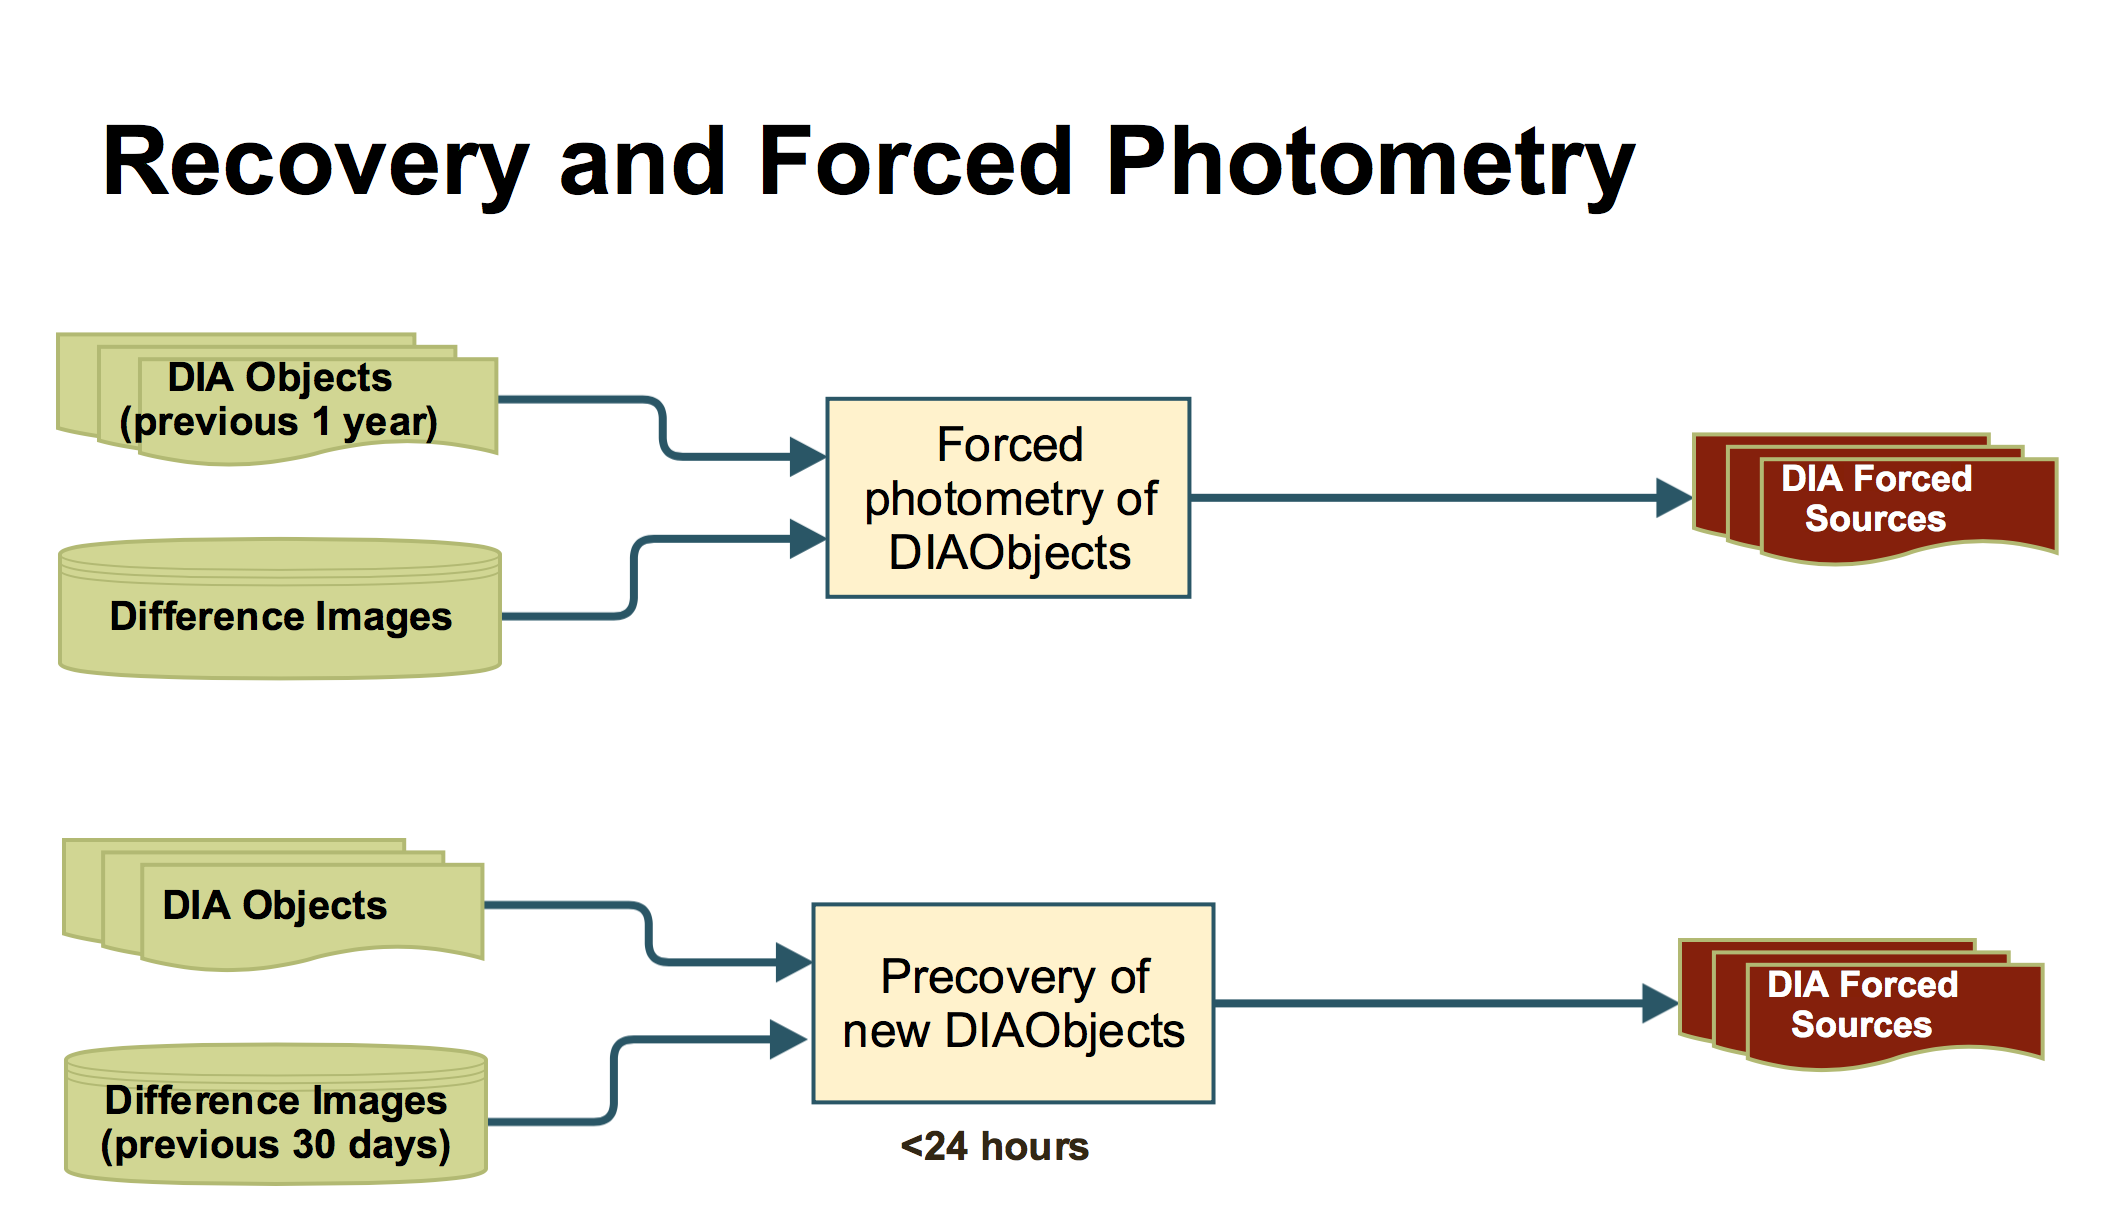
\includegraphics[width=0.9\textwidth]{figures/Forced_Precovery.png}
\caption{\label{fig:apForcedPrecovery} Forced photometry for \DIAObjects: forced photometry on a night's DiffExp for all \DIAObjects that have detected \DIASources within the last year, precovery photometry for the previous 30 days of DiffExps for new \DIAObjects}
\end{center}
\end{figure}

\begin{note}{For ZI: I moved the precovery to a single pipeline}\end{note}
\subsubsection{Input Data}

\paragraph*{Difference images:} A cache of DiffExps within a finite time interval (default 30 days) of the previous nights observations (inclusive of the previous nights data)

\paragraph*{DIAObject Database:} All \DIAObjects with a \DIASource detection within the last 12 months and all unassociated (new) \DIAObjects observed within the previous night

%\begin{note} We associate (measure forward) for 12 months but look back for 30 days\end{note}

\subsubsection{Output Data}

\paragraph*{DIAForcedSource Databases:} Forced PSF photometry at the centroid (from the aggregated individual \DIASource centroids) of a \DIAObject. The forced photometry is undertaken on the current night's DiffExp for all \DIAObjects with \DIASources detected within the last year, and on the previous 30 days of DiffExp for all newly detected \DIASources.


\subsubsection{Forced Photometry on all \DIAObjects}

Generate forced (PSF) photometry on the DiffExp for all \DIAObjects that overlap with the footprint of the CCD. Forced photometry is only generated for \DIAObjects for which there has been a \DIASource detection within the last 12 months. The forced photometry is persisted in the forced photometry table in the Level 1 database. Alerts are released prior to the generation of forced photometry and forced photometry is not released as apart of an alert which means that this component of the processing is not subject to the 60 second processing requirements for nightly processing.

\paragraph{Pipeline Tasks}

\begin{itemize}
\item Extract all \DIAObjects within the Level 1 database with a detected \DIASource within the last year (including the current nights observations). This information is available from the \DIASource and \DIAObject association.
\item For the aggregate positions within the \DIAObject undertake a PSF forced measurement as described in section \ref{sec:acForcedMeasurement}
\item Update the forced photometry tables in the Level 1 database.
\end{itemize}



\subsubsection{DIAObject Forced Photometry:}

Updated forced photometry table for all new \DIAObjects


\paragraph{Pipeline Tasks}

\begin{itemize}
\item Extract from the Level 1 database all \DIAObjects that were unassociated (i.e.\ new \DIASource detections) from the previous nights reduction. Filtering of the \DIAObjects will need to account for cases where new \DIASources are observed more than once within a night (where the second or subsequent observations do not result in a new \DIAObject).
\item Extract DiffExps within a  default 30 day window prior to the observation
\item Force photometer the extracted images as described in \ref{sec:acForcedMeasurement} using a PSF model and the centroid defined in the \DIAObject
\item Update the forced photometry table within the Level 1 database
\end{itemize}
\clearpage



\subsection{Moving Object Pipeline (\wbsMOPS)}
\label{sec:apMovingObjectPipeline}

The Moving Object Pipeline (MOPS) is responsible for generating and managing the Solar System data products. These are Solar System objects with associated Keplerian orbits, errors, and detected \DIASources. Quantitatively, it shall be capable of detecting 95\% of all Solar System objects that meet the criteria specified in the \OSS\@ (i.e.\ the observations required to define an orbit). Each visit within 10 degrees of the Ecliptic will detect approximately 4,000 asteroids.

Components of MOPS are run during and separately from nightly processing (see Figure~\ref{fig:apMOPS}). MOPS for nightly processing is described in \ref{sec:apSourceAssoc} as part of source association. ``Day MOPS'' processes newly detected \DIAObjects to search for candidate asteroid tracks. The procedure for Day-MOPS is to link \DIASource detections within a night (called tracklets), to link these tracklets across multiple nights (into tracks), to fit the tracks with an orbital model to identify those tracks that are consistent with an asteroid orbit, to match these new orbits with existing \SSObjects, and to update the \SSObject table. By its nature this process is iterative with \DIASources being associated and disassociated with \SSObjects. It is expected that a frequency of one day for these iterations (i.e.\ the \SSObjects will be update each day) will be sufficient.

\begin{figure}[th]
\begin{center}
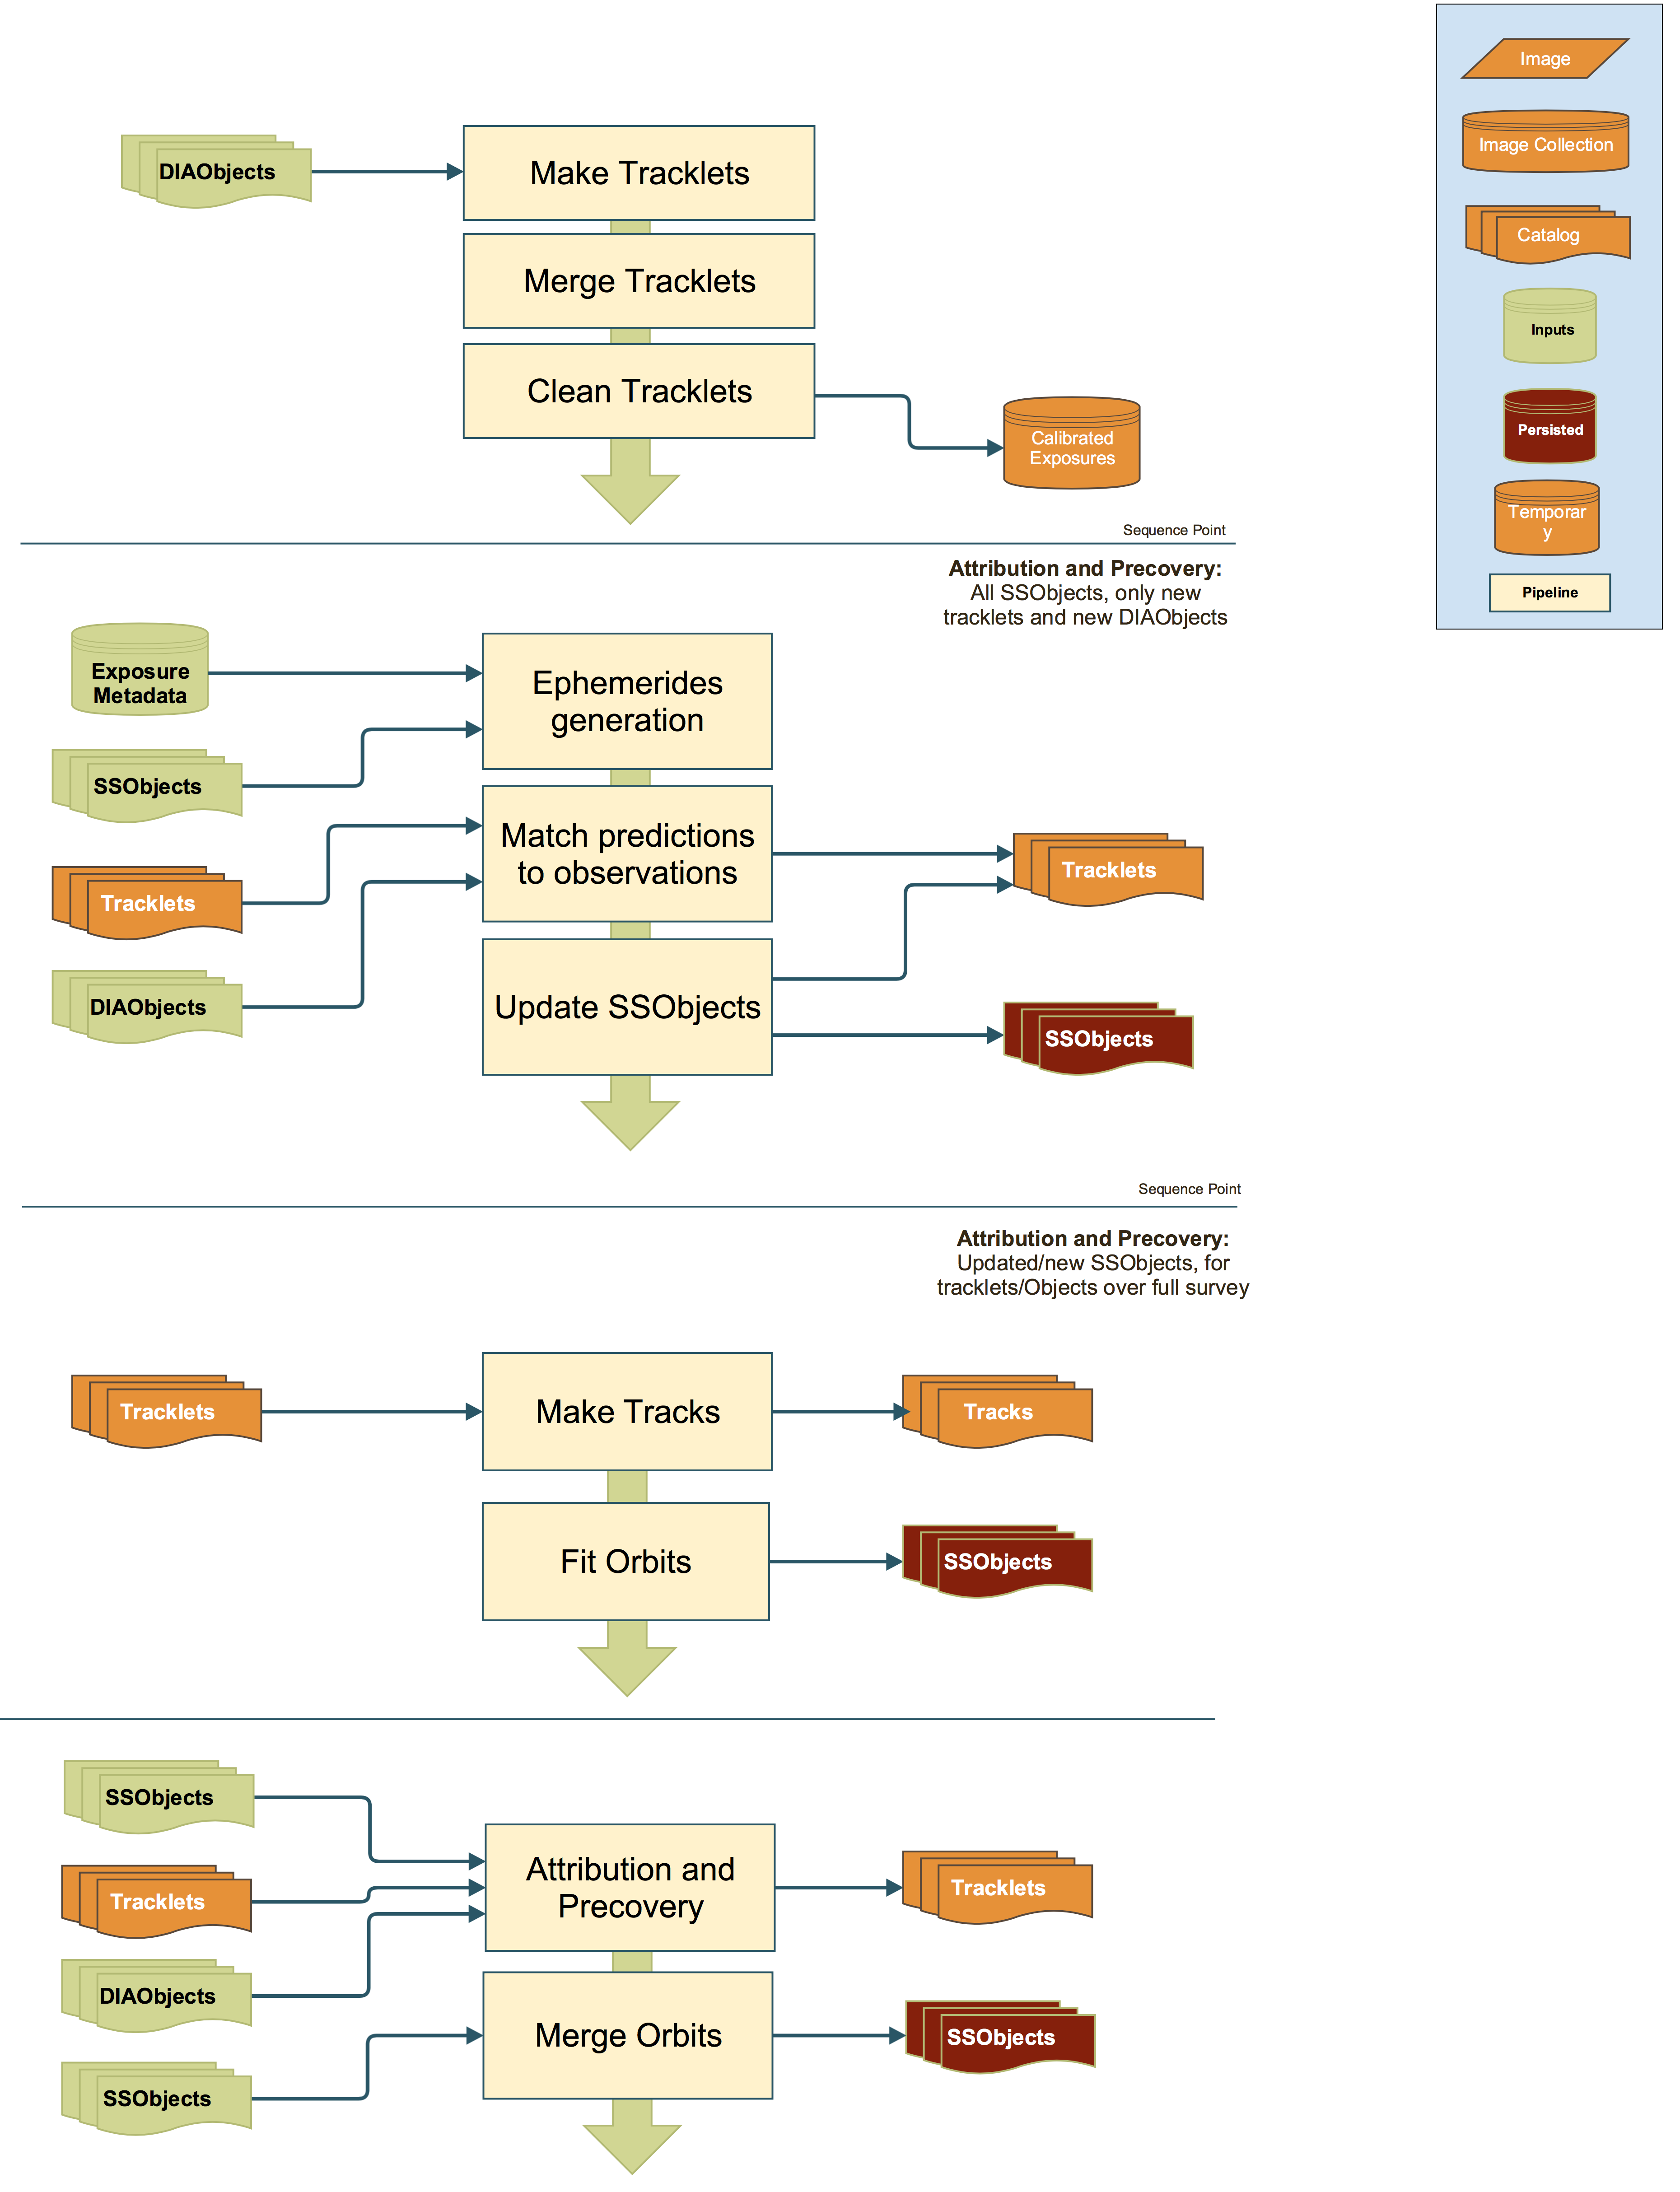
\includegraphics[width=0.9\textwidth]{figures/MOPS.png}
\caption{\label{fig:apMOPS} Detection and orbital modelling of moving sources within the nightly data: Tracklet generation from revisits, filtering of tracklets based on  known \SSObjects, fitting of tracks and orbits to tracklets, pruning of tracklets and \DIAObjects based on new and updated \SSObjects.}
\end{center}
\end{figure}

\subsubsection{Input Data}

\paragraph*{DIAObject Database: } Unassociated \DIASources from the previous night of observing.  This means \DIAObjects that were newly created during the previous night because they could not be associated with known \DIAObjects.  \DIASources associated with an \SSObject in the night are still passed through the MOPS machinery

\paragraph*{SSObject Database: } The catalog of known solar system sources

\paragraph*{Exposure Metadata:} A description of the footprint of the observations including the positions of bright stars or a model for the detection threshold as a function of position on the sky (including gaps between chips)


\subsubsection{Output Data}

\paragraph*{SSObject Database: } An updated \SSObject database with \SSObjects both added and pruned as the orbital fits are refined

\paragraph*{DIASource Database:} A updated \DIASource database with \DIASources assigned and unassigned to \SSObjects

\paragraph*{Tracklet Database:} A temporary database of tracklets measured during a night. This database will be persisted for at least a lunation.

\subsubsection{Tracklet identification}

From multiple visits within a night, link unassociated \DIASources to form tuples (or n-tuples) of \DIASources

\paragraph{Pipeline Tasks}

\begin{itemize}
\item Extract unassociated \DIASources from the Level 1 database
\item Link \DIASources into tracklets assuming a maximum velocity for the moving sources. The maximum velocity will be based on a prior as described in  \cite{2007ASPC..376..395K}. For each tracklet a velocity vector will be calculated to enable pruning or merging of degenerate tracklets within a data set.
\item Merge tracklets by clustering in velocity and position (propagated to a common visit time). Tracklets can contain multiple points and all permutations of the asteroid tuples will be stored. In the process of merging tracklets \DIASources that are not a good fit for the merged tracklet will be remove and their associated tracklets returned to the tracklet database.  Moving or trailed sources will incorporate the position angle of the source when linking. Details of the implementation of the \DIASource linkage is described in \ref{sec:acMakeTracklets}
\item Temporarily persist a database of tracklets. This database will be required for at least 30 days of data but, depending on resources available, may persist for longer.
\end{itemize}


\subsubsection{Precovery and merging of tracklets}

Tracklets are matched and merged with existing \SSObjects and removed from the Tracklet database. This culls any tracklets or \DIASources that obviously belong to an existing \SSObject from the rest of the processing.

\paragraph{Pipeline Tasks}

\begin{itemize}
\item Return all tracklets identified within a given night of observations
\item Return the footprints of each visit and the time of the observation
\item Extract \SSObjects from the \SSObject database and propagated those orbits to the position and time of a visit. Details of this orbit propagation for precovery are described in \ref{sec:acEphemerisCalculation}.
%\begin{note}What are the numbers for the \SSObject propagation and number of tracklets per visit\end{note}
\item Merge (precovery) the tracklets with the projected \SSObject trajectories and refit  the \SSObject orbit model. \DIASources previously associated with an \SSObject may no longer fit the updated \SSObject orbits. These \DIASources will be removed from the \SSObject and returned as unassociated \DIAObjects to the level 1 database. All tracklets associated with these \DIAObjects will be  returned to the tracklet database. Details of this attribution and precovery are described in \ref{sec:acAttributionAndPrecovery}
\end{itemize}

\subsubsection{Linking tracklets and orbit fitting}

Given a database of tracklets constructed from a window (default 30 days) of time, link the tracklets into tracks assuming a quadratic approximation to the trajectory. Fit these tracks with orbital models and update the \SSObject database.

\paragraph{Pipeline Tasks}

\begin{itemize}
\item Extract all tracklets from the tracklet database for a specified window in time (default 30 days)
\item Merge tracklets into tracks based on their velocities and accelerations. Candidate tracks are pruned by fitting a quadratic relation to the positions (after applying a topocentric correction to the positions of the sources). Efficiency in this matching procedure is provided by a spatial index such as a kd-tree (see \ref{sec:acOrbitFitting}).
\item Fit an orbit to each candidate track using a tool such as OOrb \\(https://github.com/oorb/oorb) and, for poorly fitting  points, return the \DIASources and associated tracklets to their respective databases for subsequent reprocessing.
\item Merge \SSObjects that have similar orbital parameters based on range searches within the six dimensional orbital parameter space.  Merged \SSObjects will need to be refit and any poorly fitting \DIASources (and associated tracklets) returned  to their respective databases for subsequent reprocessing. Details of this procedure are given in \ref{sec:acOrbitMerging}
\end{itemize}

\subsubsection{Global precovery}

For all new or updated \SSObjects propagate the orbits to the positions and times of the observations of all tracklets and orphan \DIAObjects to ``precover'' further support for the orbits. This will prune the number of tracklets and \DIAObjects that will require merging in subsequent observations.

\paragraph{Pipeline Tasks}

\begin{itemize}
\item Return all tracklets identified within a given night of observations
\item Return the footprints of each visit and the time of the observation
\item Extract orbits for all new or updated \SSObjects and propagate the positions to the times of the observations for all visits covering the extent of the tracklet database, default 30 days, (see \ref{sec:acEphemerisCalculation})
\item Merge the tracklets with the projected \SSObject positions and refit the \SSObject orbit model. Poorly fitting \DIASources (and associated tracklets) will be removed from the \SSObject and returned as unassociated \DIAObjects to the Level 1 database (as described in \ref{sec:acAttributionAndPrecovery}).
\end{itemize}


The process for precovery and updating of the \SSObject models is naturally iterative (given the pruning of poorly fitting \DIAObjects and tracklets). Updates of the \SSObjects as part of each night of operations should enable sufficient iterations without requiring Day-MOPS to be rerun multiple times per day. The computationally expensive operations in this pipeline are the orbit propagation and the orbit fitting. Resources required for orbit propagation could be reduced be removing the initial precovery stage but at the cost of increasing the number of tracklets that would be available for matching into tracks. Orbital trajectories could be pre-calculated and modelled as polynomials to enable fast interpolation during Day-MOPS.



Extending the Global Precovery to include singleton \DIASources (i.e.\ one that are not merged into tracklets) would enable the identification of asteroids at the edge of the nightly footprint (where an object moves outside of the nightly survey footprint prior to the second visit or a second visit is not obtained for a given field).

\subsubsection{Prototype Implementation}

Prototype MOPS codes are available at \url{https://github.com/lsst/mops_daymops} and \url{https://github.com/lsst/mops_nightmops}. Current DayMOPS prototype already performs within the computational envelope envisioned for LSST Operations, though it does not yet reach the required completeness requirement.


% This section is subsubsection crazy and all the whitespace ends up looking absurd.
% If needed, a similar block with the defaults can just be placed at the end of this section though.
% And if people prefer it like this, it can be moved to the preamble.
\titlespacing*{\subsubsection}
{0pt}{1ex}{0ex}


\section{Calibration Products Pipeline (\wbsCPP)}

\subsection{Key Requirements}

The work performed in this WBS serves two complementary roles:

\begin{itemize}
  \item{It will enable the production of calibration data products as required by the Level 2 Photometric Calibration Plan (\NewPCP{}) and other planning documents \cite{Lupton15}\footnote{Resolving contradictions between these documents is out of scope here.}. This includes both characterization of the sensitivity of the LSST system (optics, filters and detector) and the transmissivity of the atmosphere.}
  \item{It will characterize of detector anomalies in such a way that they can be corrected either by the instrument signature removal routines in the Single Frame Processing Pipeline (\wbsSFM) or, if appropriate, elsewhere in the system;}
  \item{It will manage and provide a catalog of optical ghosts and glints to other parts of the system upon demand.}
\end{itemize}


%%%%%%%%%%%%%%%%%%%%%%%%%%%%%%%%%%%%%%%%%%%%%%%%%%%%%%%%%%

\subsection{Inputs}

The following lists input datasets which will be available to the Calibration Products Pipeline. It should be noted that these are the raw inputs, and as such, the algorithmic sections for items that are listed as camera team deliverables are shown as ``None'', as these will already have been derived. However, many of these items are re-listed in the outputs section (\ref{sec:calibrationOutputDatasets}), where the algorithms to recalculate/monitor these on the mountain are discussed.


\subsubsection{Bias Frames}\label{inputs:biases} 
Sets of bias frames for the production of master biases.
\alg None - these just need to be taken.


\subsubsection{Gain Values}\label{inputs:gain} 
\cameraTeam
Gain values for all amplifiers;  note that these are required to high accuracy (0.1\%), as they are used while determining the photometric flats.
\alg Determination is subtle but not hard; both \fefiftyfive\ and PTC gain measurement techniques need to be applied with some care to get good results. Given the \bfeffect\ and non-linearity, it's not clear to what accuracy PTC can give gains, but \fefiftyfive\ can certainly provide gain to $\ll$0.1\% 


\subsubsection{Linearity}\label{inputs:linearityCurve} 
\cameraTeam
The linearity curve for every amplifier.
\alg None.


\subsubsection{Darks}\label{inputs:dark}
Sets of 300s dark frames.
\alg None - these just need to be taken.


\subsubsection{Crosstalk}\label{inputs:crosstalk}
\cameraTeam
The crosstalk matrix for every pair of amplifiers in the camera.
\alg None.


\subsubsection{Defect Map}\label{inputs:defectList} 
\cameraTeam
A list of all bad pixels in each CCD.
\alg None.


\subsubsection{Saturation levels}\label{inputs:saturationLevel}
\cameraTeam
The level (in electrons (or ADU?)), for each amplifier, at which charge bleeds to a neighbouring pixel. 
\alg None.


\subsubsection{Broadband Flats}\label{inputs:broadFlat}
Sets of flats taken through the standard LSST filters.  We will	need flats taken at a number of flux levels to measure brighter-fatter and check linearity.
\alg None - these just need to be taken.


\subsubsection{Monochromatic Flats}\label{inputs:monoFlat}
Sets of `monochromatic' (\c 1nm) flat-field screen images taken without the filter in the beam.
\alg None - these just need to be taken.


\subsubsection{CBP Data}\label{inputs:CBP}
Sets of \textit{C}ollimated \textit{B}eam \textit{P}rojector images. The proposed resolutions and steps in these datasets are preliminary.
\alg Scripting the CBP/8.4m to take each of these datasets in concert. The scripting/control requirements for the CBP are dealt with separately in \ref{CBP_control}.


\paragraph{CBP dataset 1}\label{inputs:CBP:mono}
Sets of CBP images scanned in wavelength at 1nm resolution every 1nm for a fixed set of spot positions on the camera, and for fixed footprint on M1.  No filter should be in the beam.
	
	
\paragraph{CBP dataset 2}\label{inputs:CBP:spot}
Sets of CBP images scanned in wavelength at 20nm resolution every 100nm, while rotating the CBP about a pupil to move the spot pattern around the camera for a fixed footprint on M1.  No filter should be in the beam.

	
\paragraph{CBP dataset 3}\label{inputs:CBP:M1}
Sets of CBP images scanned in wavelength at 20nm resolution every 100nm for a fixed set of spot positions on the camera, and for a number of footprints on M1; the minimum number of footprints is \c 6 for a 30cm CBP, but in reality we will explore more pointings to test azimuthal symmetry. No filter should be in the beam.


\paragraph{CBP dataset 4}\label{inputs:CBP:filter}
Sets of CBP images scanned in wavelength at 1nm resolution every 1nm for a fixed set of spot positions on the camera, and for fixed footprint on M1.  Repeated for every filter. \Nb the wavelength range for each scan need only cover the range for which the filter transmits appreciable light.


\paragraph{CBP dataset 5}\label{inputs:CBP:leak}
Sets of CBP images scanned in wavelength at 20nm resolution every 20nm for a fixed set of spot positions on the camera, and for fixed footprint on M1. Repeated for every filter.


\paragraph {CBP Crosstalk}\label{inputs:CBP:crosstalk}
Sets of CBP images taken with a suitable designed sparse mask to allow us to identify and measure all crosstalk images.  The simplest sparse mask would have only a single spot, used to illuminate each amplifier in the camera in turn (but less sparse solutions are probably also possible).  The wavelengths used are unimportant, and there are no constraints on beam footprints on M1 or filter choice.


\subsubsection{Filter Transmission}\label{inputs:filterTransmission}
\cameraTeam
Transmission curves for all the filters as a function of position.
\alg None.


\subsubsection{Stellar spectra}\label{inputs:starSpectrum} 
Spectrophotometrically-calibrated spectra for stars in the field of view for almost all visits.
\alg xxx Need to write this. Could potentially involve Team Stubbs/Guyonnet though.


\subsubsection{Other stellar spectra (\nb~!= \ref{inputs:starSpectrum})}\label{inputs:standardStarSpectrum}
Known spectra for bright stars in the field of view of all visits.
\alg xxx Need to write this. Could potentially involve Team Stubbs/Guyonnet though.


\subsubsection{Atmospheric Characterisation}\label{inputs:atmosphericData}
Externally measured parameters of the atmosphere, for example barometric pressure and ozone.
\alg None, except for interfacing with the site team or whoever is responsible for the equipment to automate getting these readings from the environmental monitors.


\subsubsection{Photometric Standards}\label{inputs:photometricStandards} 
Photometric standards, of a range of colours. GAIA is a likely source for these data.
\alg None.


%%%%%%%%%%%%%%%%%%%%%%%%%%%%%%%%%%%%%%%%%%%%%%%%%%%%%%%%%%
%%%%%%%%%%%%%%%%%%%%%%%%%%%%%%%%%%%%%%%%%%%%%%%%%%%%%%%%%%
%%%%%%%%%%%%%%%%%%%%%%%%%%%%%%%%%%%%%%%%%%%%%%%%%%%%%%%%%%

\subsection{Outputs from LSST's Calibration Product Pipelines \\
	/ Inputs to Alert/DRP Pipelines}
\label{sec:calibrationOutputDatasets}

This section details the output from the Calibration Products Pipeline. Algorithms for the production of each item are discussed in detail, and includes the re-derivation of the items previously just listed as camera team deliverables.

\subsubsection{Master Bias}\label{calibProducts:bias}
Trimmed, overscan subtracted, bias frame for each CCD.
\alg Construction algorithm exists in \texttt{pipe\_drivers}.

\subsubsection{Master Darks}\label{calibProducts:dark}
Trimmed, overscan subtracted, dark frame scaled to 1 second for each CCD.
\alg Construction algorithm exists in \texttt{pipe\_drivers}.


\subsubsection{Master Linearity}\label{calibProducts:linearityCurve}
Linearity curves; identical to \ref{inputs:linearityCurve}, unless updated during operations.
\alg  Will need to write algorithmic component to generate the linearity curves from raw data. Requires careful treatment as \bfeffect can masquerade as non-linearity. Code to apply non-linearity curves during \texttt{isr} is currently being implemented by Russel Owen for \texttt{obs\_decam}.


\subsubsection{Master Fringe Frames}\label{calibProducts:fringeFrames}
Some variety of fringe frames. We hope that we will not need these, but should plan for their existence as a backup.
\alg Construction of these fringe frames from \hyperref[inputs:monoFlat]{monochromatic flats} using existing algorithm in \texttt{pipe\_drivers}.


\subsubsection{Master Gain Values}\label{calibProducts:gains}
Per-amplifier gains; identical to \ref{inputs:gain}, unless updated during operations.
\alg Potentially difficult. We will have almost arbitrarily accurate gain measurements as an input, but monitoring the evolution of these gains to the required accuracy is currently an unsolved problem. Ticket \hyperref{https://jira.lsstcorp.org/browse/DM-6030}{}{}{\texttt{DM-6030}} exists to explore the possibility of using cosmic ray muons and radioisotope contamination in the camera for this purpose. If this fails (likelihood moderate-high) then another method will need to be devised.

\subsubsection{Master Defects}\label{calibProducts:defectList}
A list of all bad pixels in each CCD; identical to \ref{calibProducts:defectList}, unless updated during operations.     
\alg Statistical analysis of dark frames, flats and ``pocket-pumping" exposures will determine the defect list.


\subsubsection{Saturation Levels}\label{calibProducts:saturationLevel}
The level (in electrons (or ADU? xxx)), for each amplifier, at which charge bleeds to a neighbouring pixel; identical to \ref{calibProducts:saturationLevel}, unless updated during operations.     
\alg Easily measurable with the CBP, but need to code to detect leakage and calculate threshold level. %\rednote{Does bleeding occur in the serial register? If not, why do we expect it to be a per-amplifier thing? Could it potentially not be a per-pixel effect? This is surely known, but I should discuss with someone.}


\subsubsection{Crosstalk}\label{calibProducts:crosstalk}
The crosstalk matrix for every pair of amplifiers in the camera; identical to \ref{calibProducts:crosstalk}, unless updated during operations.
\alg The validity of \ref{calibProducts:crosstalk} is questionable to the extent where it is not clear whether it should even be a \textbf{Camera Team deliverable}. We must be able to measure this on the mountain using the CBP. The involves dithering one or more spot masks around the focal plane and measuring the coefficients. Should be highly multiplexable using a multi-pinhole mask. Need code to extract the crosstalk coefficients from these measurements.


\subsubsection{\emph{Im}pure Monochromatic Flats}\label{calibProducts:monoFlat}
Sets of `monochromatic' (\c 1nm) trimmed, overscan subtracted, flat-field images for each filter.  These flats will \textit{include} ghost and scattered light.
\alg Construction algorithm likely almost exists in \texttt{pipe\_drivers}.


\subsubsection{Pure Monochromatic Flats}\label{calibProducts:monoPhotoFlat}
Sets of `monochromatic' (\c 1nm) trimmed, overscan subtracted, flat-field images for each filter.  These flats will \textit{exclude} ghost and scattered light.
\alg Constructed from \ref{calibProducts:monoPhotoFlat} and the ghost catalogue / system optical model.


\subsubsection{PhotoFlats}\label{calibProducts:standardPhotoFlat}
The linear combination of \ref{calibProducts:monoPhotoFlat} data weighted by a flat-spectrum source (or other defined standard SED), absorbed by a standard atmosphere.
\alg Combination of \ref{calibProducts:monoPhotoFlat} should be simple; need to define the ``standard atmosphere".


\subsubsection{Low-res narrow-band flats}\label{calibProducts:monoPhotoFlatLowRes}
A low-resolution (in both space and wavelength) version of  \ref{calibProducts:monoPhotoFlat}.
\alg \rednote{Not clear to me a) why these exist and b) what a low spatial resolution flat means. Construction shouldn't be hard though.}


\subsubsection{Pixel Sizes}\label{calibProducts:pixelSizeMap} 
A map of the pixel-size distortions.  At worse, this will be a $n_{\mbox{width}}\times n_{\mbox{height}}\times 2$ datacube of floats.
\alg Algorithm to measure this is currently a (somewhat) unsolved problem. It has been shown by Aaron Roodman \& co. that these can be measured from flat-fields, but the problem is under-constrained, and thus the stability (nay, validity) of their measurements is questionable, despite seeming to work. Further thought is required to establish whether their method can be used, and if not, devise another one (though it is not obvious how the problem can be made to be well constrained). 


\subsubsection{Brighter-fatter Coefficients}\label{calibProducts:brighterFatterCoeffs}
Coefficients needed to model the brighter-fatter effects. We hope that these are a small number of floats per CCD, but this is not yet entirely clear.
\alg A number of techniques to measure these exist (mostly developed by members of the DESC SAWG). One or more of these will need to be implemented in the DM framework.

\subsubsection{Filter Transmission}\label{calibProducts:filterTransmission}
Measurement of filter transmission, measure \emph{in-situ}. As well as the filter transmission from the camera team in \ref{inputs:filterTransmission}, we further baseline the development of a procedure for measuring the filter response at 1\,nm resolution using the approach described in \cite{Lupton15}.


\subsubsection{Ghost catalog}\label{calibProducts:GhostCatalog}
A catalog of optical ghosts and glints which is available for use in other parts of the system. Detailed characterization of ghosts in the LSST system will only be possible when the system is operational. Our baseline design therefore calls for this system to be prototyped using data from precursor instrumentation; we note that ghosts in \eg HSC are well known and more significant than are expected in LSST.
\begin{note}
It is not currently clear where the responsibility for characterizing ghosts and glints in the system lies. We assume it is outwith this WBS.
\end{note}



%%%%%%%%%%%%%%%%%%%%%%%%%%%%%%%%%%%%%%%%%%%%%%%%%%%%%%%%%%
%%%%%%%%%%%%%%%%%%%%%%%%%%%%%%%%%%%%%%%%%%%%%%%%%%%%%%%%%%
%%%%%%%%%%%%%%%%%%%%%%%%%%%%%%%%%%%%%%%%%%%%%%%%%%%%%%%%%%



\subsection{CBP Control}\label{CBP_control}
The procurement of the CBP includes the procurement of the necessary control software  \rednote{Check with Patrick Ingraham that this is correct}. However, it will still remain to write scripts for the CBP and interfaces with the OCS to allow making all of the desired measurements, especially as several of these, namely \rednote{xxx, xxx \& xxx} require doing so in concert with the 8.4m.

















%
%%
%%
%
%
%
%
%
%
%


\subsection{Calibration Telescope Input Data}
\label{sec:calibrationTelescopeDatasets}
This section details to input data required to calibrate the calibration (auxiliary/Calypso) telescope itself.


\subsubsection{}\label{calypso:atmosphericAbsorption} The atmospheric absorption as a function of wavelength (at
moderate spectral resolution) for almost each visit.
\subsubsection{}\label{calypso:nightSkySpectrum} Spectrum of the night sky near the Calypso boresight, with $R
\sim 200$.\footnote{It is not entirely clear whether these will be taken on the Calypso or 8.4m	boresight.}



\subsection{Calibration Telescope Output Data}
\label{sec:calibrationTelescopeDatasets}
This section details the calibrated outputs from the calibration (auxiliary/Calypso) telescope, which, like items in section \ref{sec:calibrationOutputDatasets}, are output from to the Calibration Products Pipelines to be used in photometric calibration at various levels.


\subsubsection{}\label{calypso:atmosphericAbsorption}
The atmospheric absorption as a function of wavelength (at moderate spectral resolution) for almost each visit.
\subsubsection{}\label{calypso:nightSkySpectrum}
Spectrum of the night sky near the Calypso boresight, with $R\sim 200$.\footnote{It is not entirely clear whether these will be taken on the Calypso or 8.4m boresight.}

\Nb these are clearly not raw data, but will need to be extracted from spectrographic exposures.
\XXX{Add a description of those pipelines, and of the input data that they require.}



%%%%%%%%%%%%%%%%%%%%%%%%%%%%%%%%%%%%%%%%%%%%%%%%%%%%%
%%%%%%%%%%%%%%%%%%%%%%%%%%%%%%%%%%%%%%%%%%%%%%%%%%%%%
%%%%%%%%%%%%%%%%%%%%%%%%%%%%%%%%%%%%%%%%%%%%%%%%%%%%%


\subsection{Prototype Implementation}

While parts of the Calibration Products Pipeline have been prototyped by the LSST Calibration Group (see the \NewPCP for discussion), these have not been written using LSST Data Management software framework or coding standards. We therefore expect to transfer the know-how, and rewrite the implementation.













\subsection{Overview of calibration procedure}
This section, whilst not strictly concerning the \emph{production} of the calibration products themselves, aims to give a broad overview of how these products will be used and why. 
\begin{note}
Whilst this isn't technically part of the CPP remit, without it, all that is here is a list of ingredients, (and how to make the compound ingredients), with no overview of the recipe, which makes for a strange section in a cookbook. If this is no desired or should live somewhere else then feel free to move or \emph{re}move it, but I felt like it should be in here as this stuff is not easy to get ones head around at the best of times.
\end{note}

Overview goes here! xxx

%\paragraph{Instrumental sensitivity}
%
%
%
%
%\begin{enumerate}
%  \item{Record bias/dark frames;}
%  \item{Use ``monochromatic'' (1\,nm) flat field screen flats with no filter in the beam to measure the per-pixel sensitivity;}
%  \item{Use a collimated beam projector (CBP) to measure the quantum efficiency (QE) at a set of points in the focal plane, dithering those points to tie them together;}
%  \item{Combine the screen and CBP data to determine the broad band (10--100\,nm) QE of all pixels;}
%  \item{Fold in the filter response to determine the 1\,nm resolution effective QE of all pixels.}
%\end{enumerate}
%
%This WBS is responsible for the development of the data analysis algorithms and software required and the ultimate delivery of the flat fields. Development and commissioning of the CBP itself, together with any other infrastructure required to perform the above procedure, lies outwith Data Management (see 04C.08 \emph{Calibration System}).
%
%\paragraph{Atmospheric transmissivity}
%
%Measurements from the auxiliary instrumentation---to include the 1.2\,m ``Calypso'' telescope, a bore-sight mounted radiometer and satellite-based measurement of atmospheric parameters such as pressure and ozone---will be used to determine the atmospheric absorption along the line of sight to standard stars. The atmospheric transmission will be decomposed into a set of basis functions and interpolated in space in time to any position in the LSST focal plane.
%
%This WBS will develop a pipeline for accurate spectrophotometric measurement of stars with the auxiliary telescope. We expect to repurpose and build upon publicly available code e.g.\ from the PFS\footnote{Subaru's Prime Focus Spectrograph; \url{http://sumire.ipmu.jp/pfs/}.} project for this purpose.
%
%This WBS will construct the atmospheric model, which may be based either on \textsc{modtran} (as per \NewPCP{}) or a PCA-like decomposition of the data (suggested by \cite{Lupton15}).
%
%This WBS will define and develop the routine for fitting the atmospheric model to each exposure from the calibration telescope and providing estimates of the atmospheric transmission at any point in the focal plane upon request.
%
%\paragraph{Detector effects}
%
%An initial cross-talk correction matrix will be determined by laboratory measurements on the Camera Calibration Optical Bench (CCOB). However, to account for possibile instabilities, this WBS will develop an on-telescope method. We baseline this as being based on measurement with the CBP, but we note the alternative approach based on cosmic rays adopted by HSC \cite{Furusawa14}.
%
%Multiple reflections between the layers of the CCD give rise to spatial variability with fine scale structure in images which may vary with time \cite[\S2.5.1]{Lupton15}. These can be characterized by white light flat-fields. Preliminary analysis indicates that these effects may be insignificant in LSST \cite{Rasmussen15}; however, the baseline calls for a routine developed in this WBS to analyse the flat field data and generate fringe frames on demand. This requirement may be relaxed if further analysis (outside the scope of this WBS) demonstrates it to be unnecessary.
%
%
%This WBS will develop algorithms to characterize and mitigate anomalies due to the nature of the camera's CCDs.
%
%\begin{note}
%There's a complex inter-WBS situation here: the actual mitigation of CCD anomalies will generally be performed in SFM (\wbsSFM{}), based on products provided by this WBS which, in turn, may rely on laboratory based research which is broadly outside the scope of DM\@. We baseline the work required to develop the corrective algorithms here. We consider moving it to \wbsSFM{} in future.
%\end{note}
%
%The effects we anticipate include:
%
%\begin{itemize}
%  \item{QE variation between pixels;}
%  \item{Static non-uniform pixel sizes (e.g.\ ``tree rings'' \cite{Stubbs14});}
%  \item{Dynamic electric fields (e.g.\ ``brighter-fatter'' \cite{Antilogus14});}
%  \item{Time dependent effects in the camera (e.g.\ hot pixels, changing cross-talk coefficients);}
%  \item{Charge transfer (in)efficiency (CTE).}
%\end{itemize}
%
%Laboratory work required to understand these effects is outwith the scope of this WBS\@. In some cases, this work may establish that the impact of the effect may be neglected in LSST\@. The baseline plan addresses these issues through the following steps:
%
%\begin{itemize}
%  \item{Separate QE from pixel size variations\footnote{Refer to work by Rudman.} and model both as a function of position (and possibly time);}
%  \item{Learn how to account for pixel size variation over the scale of objects (e.g.\ by redistributing charge);}
%  \item{Develop a correction for the brighter-fatter effect and develop models for any features which cannot be removed;}
%  \item{Handle edge/bloom using masking or charge redistribution;}
%  \item{Track defects (hot pixels);}
%  \item{Handle CTE, including when interpolating over bleed trails.}
%\end{itemize}
%


%

%Produce Master Pupil Ghost Exposure; Determine CCOB-derived Illumination Correction; Determine Optical Model-derived Illumination Correction; Determine Star Raster Photometry-derived Illumination Correction; Create Master Illumination Correction; Determine Self-calibration Correction-Derived Illumination Correction; Correct Monochromatic Flats; Reduce Spectrum Exposure




\subsection{UNSTRUCTURED OPEN QUESTIONS \\ a.k.a. Merlin's random thoughts/ramblings}

This section is just things that I thought of whilst working through this document. They probably don't even belong in here at all, but I wanted to capture them and this seemed a semi-relevant place (and Jim started it!).
\begin{itemize}
	\item test
	\item test 2
\end{itemize}





\clearpage































%%%%%%%%%%%%%%%%%%%%%%%%%%%%%%%%%%%%%%%%%%%%%%%%%%%
%%%%%%%%%%%%%%%%%%%%%%%%%%%%%%%%%%%%%%%%%%%%%%%%%%%
%%%%%%%%%%%%%%%%%%%%%%%%%%%%%%%%%%%%%%%%%%%%%%%%%%%



%\section{Photometric Calibration Pipeline (\wbsPhotoCal)}
%
%\subsection{Key Requirements}
%
%The Photometric Calibration Pipeline is required to internally calibrate the relative photometric zero-points of every observation, enabling the Level 2 catalogs to reach the required SRD precision.
%
%\subsection{Baseline Design}
%
%The adopted baseline algorithm is a variant of ``ubercal'' \cite{Padmanabhan08, Schlafly12}. This baseline is described in detail in the Photometric Self Calibration Design and Prototype Document (\UCAL).
%
%\subsection{Constituent Use Cases and Diagrams}
%
%Perform Global Photometric Calibration;
%
%\subsection{Prototype Implementation}
%
%Photometric Calibration Pipeline has been fully prototyped by the LSST Calibration Group to the required level of accuracy and performance (see the \UCAL document for discussion). % RHL really?  I thought that they wrote a small-scale toy version.  But I may be totally out of date.
%\\
%
%As the prototype has not been written using LSST Data Management software framework or coding standards, we assume a non-negligible refactoring and coding effort will be needed to convert it to production code in LSST Construction.
%
%\clearpage
%
%\section{Astrometric Calibration Pipeline (\wbsAstroCal)}
%
%\subsection{Key Requirements}
%
%The Astrometric Calibration Pipeline is required to calibrate the relative and absolute astrometry of the LSST survey, enabling the Level 2 catalogs to reach the required SRD precision.
%
%\subsection{Baseline Design}
%
%Algorithms developed for the Photometric Calibration Pipeline (\wbsPhotoCal) will be repurposed for astrometric calibration by changing the relevant functions to minimize. This pipeline will further be aided by WCS and local astrometric registration modules developed as a component of the Single Frame Processing pipeline (\wbsSFM).
%\\
%
%Gaia standard stars will be used to fix the global astrometric system. It is likely that the existence of Gaia catalogs may make a separate Astrometric Calibration Pipeline unnecessary.
%
%\subsection{Constituent Use Cases and Diagrams}
%
%Perform Global Astrometric Calibration;
%
%\subsection{Prototype Implementation}
%
%The Astrometric Calibration Pipeline has been partially prototyped by the LSST Calibration Group, but outside of LSST Data Management software framework. We expect to transfer the know-how, and rewrite the implementation.

\section{Data Release Production}
\label{sec:drp}

\begin{figure}
\centering
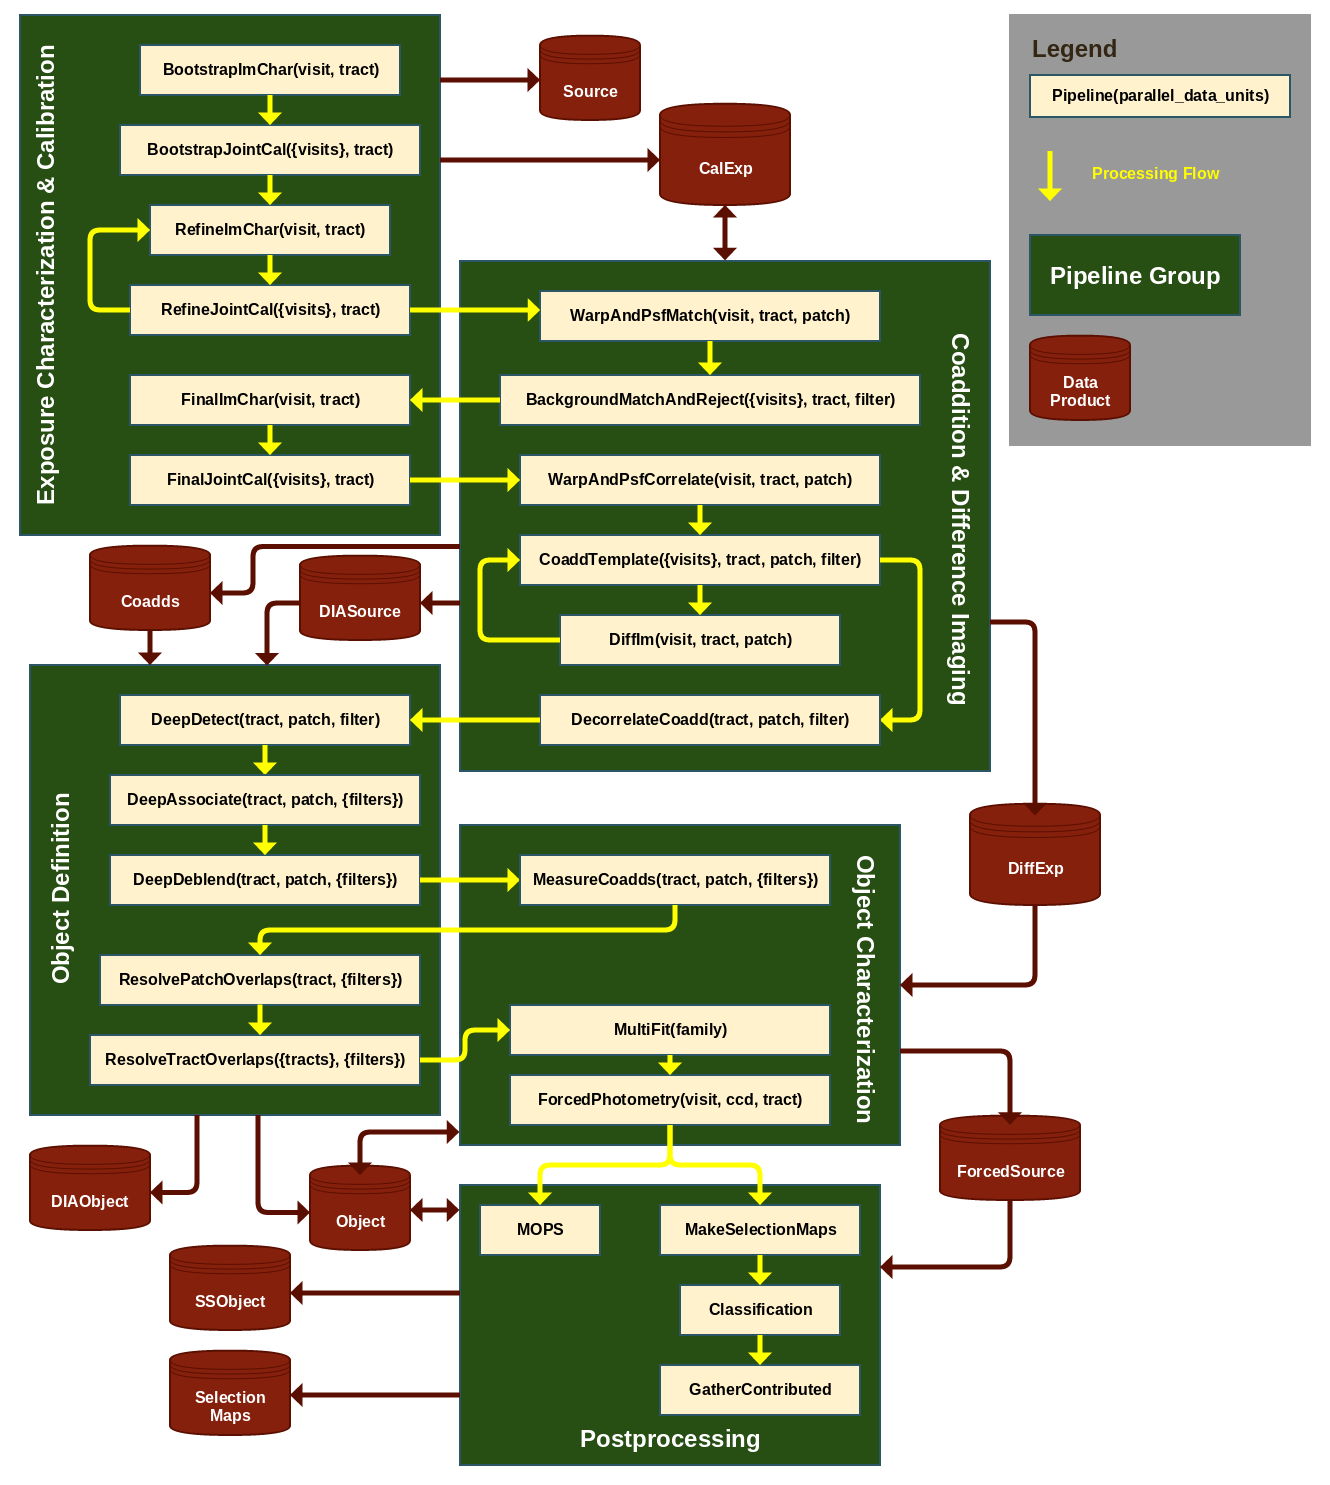
\includegraphics[width=\textwidth]{figures/drp_summary.png}
\caption{Summary of the Data Release Production processing flow.  Processing is split into multiple pipelines, which are conceptually organized into the groups discussed in sections~\ref{sec:drp_imchar_and_jointcal}-\ref{sec:drp_postprocessing}.
\label{fig:drp_summary}}
\end{figure}

\begin{note}[TODO]
  Update figure to reflect changes to sections in text.
\end{note}

A Data Release Production is run every year (twice in the first year of operations) to produce a set of catalog and image data products derived from all observations from the beginning of the survey to the point the production began.  This includes running a variant of the difference image analysis run in Alert Production, in addition to direct analysis of individual exposures and coadded images.  The data products produced by a Data Release Production are summarized in table~\ref{table:drp_data_products}.


\begin{table}
\small
\begin{tabularx}{\textwidth}{ | l | l | X | }
  \hline
  {\bf Name} & {\bf Availability} & {\bf Description} \\
  \hline
  Source & Stored &
  Measurements from direct analysis of individual exposures. \\
  \hline
  DIASource & Stored &
  Measurements from difference imagine analysis of individual exposures. \\
  \hline
  Object & Stored &
  Measurements for a single astrophysical object, derived from all available information, including coadd measurements, simultaneous multi-epoch fitting, and forced photometry.  Does not include solar system objects. \\
  \hline
  DIAObject& Stored &
  Aggregate quantities computing by associating spatially colocated DIASources. \\
  \hline
  ForcedSource & Stored &
  Flux measurements on each direct and difference image at the position of every Object. \\
  \hline
  SSObject & Stored &
  Solar system objects derived by associating DIASources and inferring their orbits. \\
  \hline
  CalExp & Regenerated &
  Calibrated exposure images for each CCD/visit (sum of two snaps). \\
  \hline
  DiffExp & Regenerated &
  Difference between CalExp and PSF-matched template coadd. \\
  \hline
  DeepCoadd & Stored &
  Coadd image with a reasonable combination of depth and resolution. \\
  \hline
  EpochRangeCoadd & Renegerated &
  Coadd image that cover only a limited range of epochs. \\
  \hline
  BestSeeingCoadd & Regenerated &
  Coadd image built from only the best-seeing images. \\
  \hline
  PSFMatchedCoadd & Regenerated &
  Coadd image with a constant, predetermined PSF. \\
  \hline
\end{tabularx}
\caption{Table of public data products produced during a Data Release Production.  A full description of these data products can be found in the Data Products Definition Document (LSE-163).
\label{table:drp_data_products}}
\end{table}

From a conceptual standpoint, data release production can be split into five groups of pipelines, executed in approximately the following order:
\begin{enumerate}
\item We characterize and calibrate each exposure, estimating point-spread functions, background models, and astrometric and photometric calibration solutions.  This iterates between processing individual exposures independently and jointly fitting catalogs derived from multiple overlapping exposures.  These steps are described more fully in section~\ref{sec:drp_imchar_and_jointcal}.
\item We alternately combine images and subtract them, using differences to find artifacts and time-variable sources while building coadds that produce a deeper view of the static sky.  Coaddition and difference imaging is described in section~\ref{sec:drp_coaddition_and_diffim}.
\item After all image processing is complete, we run additional catalog-only pipelines to fill in additional object properties.  Unlike previous stages, this postprocessing is not localized on the sky, as it may use statistics computed from the full data release to improve our characterization of individual objects.  Postprocessing pipelines are described in section~\ref{sec:drp_postprocessing}.
\end{enumerate}
This conceptual ordering is an oversimplification of the actual processing flow, however; as shown in Figure~\ref{fig:drp_summary}, pipeline groups are actually interleaved.

Each pipeline in this the diagram represents a particular piece of code excuted in parallel on a specific unit of data, but pipelines may contain additional (and more complex) parallelization to further subdivide that data unit.  The processing flow also includes the possibility of iteration between pipelines, indicated by cycles in the diagram.  The number of iterations in each cycle will be determined (via tests on smaller productions) before the start of the production, allowing us to remove these cycles simply by duplicating some pipelines a fixed number of times.  The final data release production processing can thus be described as a directed acyclic graph (DAG) to be executed by the orchestration middleware, with pipelines as edges and (intermediate) data products as vertices.  Most of the graph will be generated by applications code before the production begins, using a format and/or API defined by the orchestration middleware.  Howver, some parts of the graph must be generated on-the-fly; this will be discussed further in section~\ref{sec:drpMultiFit}.


\subsection{Image Characterization and Calibration}
\label{sec:drp_imchar_and_jointcal}

\begin{note}[ImChar/JointCal Diagram]
Extract ImChar/JointCal pipelines from ``DRP Top-Level Overview'' on confluence and expand detail to show data flow and ordering of ``Task/Process'' boxes.
\end{note}

The first steps in a Data Release Production characterize the properties of individual exposures, by iterating between pixel-level processing of individual visits (``ImChar'', or ``Image Characterization'' steps) and joint fitting of all catalogs overlapping a tract (``JointCal'', or ``Joint Calibration'' steps).  All ImChar steps involve fitting the PSF model and measuring Sources (gradually improving these as we iterate), while JointCal steps fit for new astrometric (WCS) and photometric solutions while building new reference catalogs for the ImChar steps.  Iteration is necessary for a few reasons:
\begin{itemize}
\item The PSF and WCS must have a consistent definition of object centroids.  Celestial positions from a reference catalog are transformed via the WCS to set the positions of stars used to build the PSF model, but the PSF model is then used to measure debiased centroids that feed the WCS fitting.
\item The later stages of photometric calibration and PSF modeling require secure star selection and colors to infer their SEDs.  Magnitude and morphological measurements from ImChar stages are aggregated the reference catalog in the subsequent JointCal stage, allowing these colors and classifications to be used for PSF modeling in the following ImChar stage.
\end{itemize}

The ImChar and JointCal iteration is itself interleaved with background matching and difference imaging, as described in section~\ref{sec:drp_coaddition_and_diffim}.  This allows the better backgrounds and masks to be defined by comparisons between images before the final Source measurements, image characterizations, and calibrations.

Each ImChar pipeline runs on a single visit, and each JointCal pipeline runs simultaneously on all visits within a single tract, allowing tracts to be run entirely independently.

The final output data products of the ImChar/JointCal iteration are the Source table and most of the CalExp (calibrated exposure) images.  CalExp is an \hyperref[sec:spImagesExposure]{Exposure}, and hence has Image, Mask, Variance, Background, PSF, WCS, and PhotoCalib components that we will track separately.

\subsubsection{BootstrapImChar}
\label{sec:drpBootstrapImChar}

The BootstrapImChar pipeline is the first thing run on each science exposure in a data release.  It has the difficult task of bootstrapping multiple quantities (PSF, WCS, photometric calibration, background model, etc.) that each normally require all of the others to be specified when one is fit.  As a result, while the algorithmic components to be run in this pipeline are generally clear, their ordering and specific requirements are not; algorithms that are run early will have a harder task than algorithms that are run later, and some iteration will almost certainly be necessary.

A plausible (but by no means certain) high-level algorithm for this pipeline is given below in pseudocode.  Highlighted terms are described in more detail below the pseudocode block.

\lstset{
    language=Python,
    basicstyle=\scriptsize\ttfamily,
    keywordstyle=\bfseries,
    commentstyle=\color{darkgray},
    escapeinside={\%}{\%},
}

% Define a local macro that lets us refer to sections of the text
% more easily (will undefine at the end of this section).
\newcommand{\hr}[1]{\hyperref[sec:drpBootstrapImChar_#1]{#1}}

\begin{lstlisting}
def BootstrapImChar(%\hr{raw}%, %\hr{reference}%):
    # Some data products components are visit-wide and some are per-CCD;
    # these imaginary data types lets us deal with both.
    # VisitExposure also has components; most are self-explanatory, and
    # {mi} == {image,mask,variance} (for "MaskedImage").
    calexp = VisitExposure()
    sources = VisitCatalog()
    snaps = VisitMaskedImageList()  # holds both snaps, but only {image,mask,variance}
    parallel for ccd in ALL_SENSORS:
        snaps[ccd] = [%\hr{RunISR}%(raw[ccd]) for snap in SNAP_NUMBERS]
        snaps[ccd].mask = %\hr{SubtractSnaps}%(snaps[ccd])
        calexp[ccd].mi = %\hr{CombineSnaps}%(snaps[ccd])
    calexp.psf = %\hr{FitWavefront}%(calexp[WAVEFRONT_SENSORS].mi)
    calexp.{image,mask,variance,background}
        = %\hr{SubtractBackground}%(calexp.mi)
    parallel for ccd in ALL_SENSORS:
        sources[ccd] = %\hr{DetectSources}%(calexp.{mi,psf})
    sources[ccd] = %\hr{DeblendSources}%(sources[ccd], calexp.{mi,psf})
    sources[ccd] = %\hr{MeasureSources}%(sources[ccd], calexp.{mi,psf})
    matches = %\hr{MatchSemiBlind}%(sources, reference)
    while not converged:
        %\hr{SelectStars}%(matches, exposures)
        calexp.wcs = %\hr{FitWCS}%(matches, sources, reference)
        calexp.psf = %\hr{FitPSF}%(matches, sources, calexp.{mi,wcs})
        %\hr{WriteDiagnostics}%(snaps, calexp, sources)
        parallel for ccd in ALL_SENSORS:
            snaps[ccd] = %\hr{SubtractSnaps}%(snaps[ccd], calexp[ccd].psf)
            calexp[ccd].mi = %\hr{CombineSnaps}%(snaps[ccd])
            calexp[ccd].mi = %\hr{SubtractStars}%(calexp[ccd].{mi,psf}, sources[ccd])
        calexp.{mi,background} = %\hr{SubtractBackground}%(calexp.mi)
        parallel for ccd in ALL_SENSORS:
            sources[ccd] = %\hr{DetectSources}%(calexp.{mi,psf})
            calexp[ccd].mi, sources[ccd] =
                %\hr{ReinsertStars}%(calexp[ccd].{mi,psf}, sources[ccd])
            sources[ccd] = %\hr{DeblendSources}%(sources[ccd], calexp.{mi,psf})
            sources[ccd] = %\hr{MeasureSources}%(sources[ccd], calexp.{mi,psf})
        matches = %\hr{MatchNonBlind}%(sources, reference)
    calexp.psf.apcorr = %\hr{FitApCorr}%(matches, sources)
    parallel for ccd in SCIENCE_SENSORS:
        sources[ccd] = %\hr{ApplyApCorr}%(sources[ccd], calexp.psf)
    return calexp, sources
\end{lstlisting}

\paragraph{Input Data Product: Raw}
\label{sec:drpBootstrapImChar_raw}

Raw amplifier images from science and wavefront CCDs, spread across one or more snaps.  Needed telescope telemetry (seeing estimate, approximate pointing) is assumed to be included in the raw image metadata.

\paragraph{Input Data Product: Reference}
\label{sec:drpBootstrapImChar_reference}

A full-sky catalog of reference stars derived from both external (e.g. Gaia) and LSST data.

The \hyperref[sec:drpStandardJointCal]{StandardJointCal} pipeline will later define a deeper reference catalog derived from this one and the new data being processed, but the origin and depth of the initial reference catalog is largely TBD.  It will almost certainly include Gaia stars, but it may also include data from other telescopes, LSST special programs, LSST commissioning observations, and/or the last LSST data release.  Decisions will require some combination of negotation with the LSST commissioning team, specification of the special programs, quality analysis and experimentation with the Gaia catalog, and policy decisions from DM leadership on the degree to which data releases are required to be independent.  Depending on the choices selected, it could also require a major separate processing effort using modified versions of the data release production pipelines.

\paragraph{Output Data Product: Source}
\label{sec:drpBootstrapImChar_sources}

A preliminary version of the Source table.  This could contain all of the columns in the DPDD Source schema if the \hr{MeasureSources} is appropriately configured, but some of these columns are likely unnecessary in its role as an intermediate data product that feeds \hyperref[sec:drpStandardJointCal]{StandardJointCal}, and it is likely that other non-DPDD columns will be present for that role.

BootstrapImChar also has the capability to produce even earlier versions of the Source table for diagnostic purposes (see \hr{WriteDiagnostics}).  These tables are not associated with any photometric calibration or aperture correction, and some may not have any measurements besides centroids, and hence are never substitutable for the final Source table.

\paragraph{Output Data Product: CalExp}
\label{sec:drpBootstrapImChar_calexp}

A preliminary version of the CalExp (calibrated direct exposure).  CalExp is an \hyperref[sec:spImagesExposure]{Exposure} object, and hence it has several components.  BootstrapImChar is the only pipeline that actually updates all of them.  Some CalExp components are determined at the scale of a full FoV and hence should probably be persisted at the visit level (PSF, WCS, PhotoCalib, Background), while others are straightforward CCD-level data products (Image, Mask, Variance).

\paragraph{RunISR}
\label{sec:drpBootstrapImChar_RunISR}

Delegate to the \hyperref[sec:acISR]{ISR algorithmic component} to perform standard detrending as well as brighter-fatter correction and interpolation for pixel-area variations (\hyperref[sec:acFixPixelAreaVariations]{Warping Irregularly-Sampled Images}).  It is possible that these corrections will require a PSF model, and hence must be backed-out and recorrected at a later stage when an improved PSF model is available.

We assume that the applied flat field is appropriate for background estimation.

\paragraph{SubtractSnaps}
\label{sec:drpBootstrapImChar_SubtractSnaps}

Delegate to the \hyperref[sec:acSnapSubtraction]{Snap Subtraction algorithmic component} to mask artifacts in the difference between snaps.  If passed a PSF (as in the second call), also interpolate them by delegating to the \hyperref[sec:acArtifactInterpolation]{Artifact Interpolation} algorithmic component.

We assume here that the PSF modeled on the combination of the two Snaps is sufficient for interpolation on the Snaps individually; if this is not true, we can just mask and interpolate both Snaps when an artifact appears on either of them (or we could do per-Snap PSF estimation, but that's a lot more work for very little gain).

\paragraph{CombineSnaps}
\label{sec:drpBootstrapImChar_CombineSnaps}

Delegate to the \hyperref[sec:acCoaddition]{Image Coaddition algorithmic component} to combine the two Snaps while handling masks appropriately.

We assume there is no warping involved in combining snaps.  If this is needed, we should instead advocate for dropping snaps in favor of a a single longer exposure.

\paragraph{FitWavefront}
\label{sec:drpBootstrapImChar_FitWavefront}

Delegate to the \hyperref[sec:acWavefrontSensorPSF]{Wavefront Sensor PSF algorithmic component} to generate an approximate PSF using only data from the wavefront sensors and observational metadata (e.g. reported seeing).

Processing the wavefront sensors will likely require some form of detection and measurement; we currently consider this to be part of the \hyperref[sec:acWavefrontSensorPSF]{Wavefront Sensor PSF} code, though it may delegate to e.g. \hyperref[sec:acSourceDetection]{Source Detection} and/or \hyperref[sec:acSingleFrameMeasurement]{Single Frame Measurement}.

The required quality of this PSF estimate is TBD; setting preliminary requirements will involve running a version of BootstrapImChar with at least mature detection and PSF-modeling algorithms on precursor data taken in crowded fields, and final requirements will require proceessing full LSST camera data in crowded fields.  However, robustness to poor data quality and crowding is much more important than accuracy; this stage need only provide a good enough result for subsequent stages to prcoeed.

\paragraph{SubtractBackground}
\label{sec:drpBootstrapImChar_SubtractBackground}

Delegate to the \hyperref[sec:acBackgroundEstimation]{Background Estimation} algorithmic component to model and subtract the background consistently over the full field of view.

The multiple backgrounds subtracted in BootstrapImChar may or may not be cumulative (i.e. we may or may not add the previous background back in before estimating the latest one).

\paragraph{DetectSources}
\label{sec:drpBootstrapImChar_DetectSources}

Delegate to the \hyperref[sec:acSourceDetection]{Source Detection algorithmic component} to find above-threshold regions (\hyperref[sec:spFootprints]{Footprints}) and peaks within them in a PSF-correlated version of the image.

In crowded fields, each iteration of detection will decrease the threshold, increasing the number of objects detection.  Because this will treat fluctuations in the background due to undetected objects as noise, we may need to extend PSF-correlation to the appropriate filter for an image with correlated noise and characterize the noise field from the image itself.

Because we will use wavefront data to constrain the PSF, we also run detection on the wavefront sensors.  It is possible that this will require a different algorithmic component if we cannot just treat the wavefront sensors as science sensors with an out-of-focus PSF.

\paragraph{DeblendSources}
\label{sec:drpBootstrapImChar_DeblendSources}

Delegate to the \hyperref[sec:acSingleFrameDeblending]{Single Frame Deblending algorithmic component} to split \hyperref[sec:spFootprints]{Footprints} with multiple peaks into deblend families.

Because we will use wavefront data to constrain the PSF, we also run deblending on the wavefront sensors.  It is possible that this will require a different algorithmic component if we cannot just treat the wavefront sensors as science sensors with an out-of-focus PSF, and we need deblending to extract wavefront information.

\paragraph{MeasureSources}
\label{sec:drpBootstrapImChar_MeasureSources}

Delegate to the \hyperref[sec:acSingleFrameMeasurement]{Single Frame Measurement algorithmic component} to measure source properties.

In BootstrapImChar, we anticipate using the \hyperref[sec:acReplaceNeighborsWithNoise]{Neighbor Noise Replacement} approach to deblending, with the following plugin algorithms:
\begin{itemize}
\item \hyperref[sec:acCentroidAlgorithms]{Centroids}
\item \hyperref[sec:acShapeAlgorithms]{Second-Moment Shapes}
\item \hyperref[sec:acPixelFlags]{Pixel Flag Aggregation}
\item \hyperref[sec:acAperturePhotometry]{Aperture Photometry} (but only for one or two radii)
\item \hyperref[sec:acStaticPointSourceModels]{Static Point Source Models}
\end{itemize}

Because we will use wavefront data to constrain the PSF, we also run measurement on the wavefront sensors (but probably without any flux measurement algorithms, and perhaps with modified versions of other algorithms).  It is possible that this will require a different algorithmic component if we cannot just treat the wavefront sensors as science sensors with an out-of-focus PSF.

\paragraph{MatchSemiBlind}
\label{sec:drpBootstrapImChar_MatchSemiBlind}

Delegate to the \hyperref[sec:acSingleVisitReferenceMatching]{Single Visit Reference Matching algorithmic component} to match source catalogs to a global reference catalog.  This occurs over the full field of view, ensuring robust matching even when some CCDs have no matchable stars due to crowding, flux limits, or artifacts.

``Semi-Blind'' refers to the fact that the WCS is not yet well known (all we have is what is provided by the observatory), so the matching algorithm must account for an unknown (but small) offset between the WCS-predicted sources positions and the reference catalog positions.

\paragraph{SelectStars}
\label{sec:drpBootstrapImChar_SelectStars}

Use reference catalog classifications and source flags to select a clean sample stars to use for later stages.

If we decide not to rely on a pre-existing reference catalog to separate stars from galaxies and other objects, we will need a new algorithmic component to select stars based on source measurements.

\paragraph{FitWCS}
\label{sec:drpBootstrapImChar_FitWCS}

Delegate to the \hyperref[sec:acSingleVisitAstrometricFit]{Single Visit Astrometric Fit algorithmic component} to determine the WCS of the image.

We assume this works by fitting a simple mapping from the visit's focal plane coordinate system to the sky and composing it with the (presumed fixed) mapping between CCD coordinates and focal plane coordinates.  This fit will be improved in later pipelines, so it does not need to be exact; $<$0.05 arcsecond accuracy should be sufficient.

As we iterate in crowded fields, the number of degrees of freedom in the WCS should be allowed to slowly increase.

\paragraph{FitPSF}
\label{sec:drpBootstrapImChar_FitPSF}

Delegate to the \hyperref[sec:acFullVisitPSF]{Full Visit PSF Modeling algorithmic component} to construct an improved PSF model for the image.

Because we are relying on a reference catalog to select stars, we should be able to use colors from the reference catalog to estimate SEDs an include wavelength dependence in the fit.  If we do not use a the reference catalog early in BootstrapImChar, PSF estimation here will not be wavelength-dependent.  In either case the PSF model will be further improved in later pipelines.

PSF estimation at this stage must include some effort to model the wings of bright stars, even if this is tracked and constrained separately from the model for the core of the PSF.

As we iterate in crowded fields, the number of degrees of freedom in the PSF model should be allowed to slowly increase.

\paragraph{WriteDiagnostics}
\label{sec:drpBootstrapImChar_WriteDiagnostics}

If desired, the current state of the \texttt{source}, \texttt{calexp}, and \texttt{snaps} variables may be persisted here for diagnostic purposes.

\paragraph{SubtractStars}
\label{sec:drpBootstrapImChar_SubtractStars}

Subtract all detected stars above a flux limit from the image, using the PSF model.  In crowded fields, this should allow subsequent \hr{SubtractBackground} and \hr{DetectSources} steps to push fainter by removing the brightest stars in the image.

Sources classified as extended are never subtracted.

\paragraph{ReinsertStars}
\label{sec:drpBootstrapImChar_ReinsertStars}

Add stars removed in \hr{SubtractStars} back into the image, and merge corresponding \hyperref[sec:spFootprints]{Footprints} and peaks into the source catalog.

\paragraph{MatchNonBlind}
\label{sec:drpBootstrapImChar_MatchNonBlind}

Match a single-CCD source catalog to a global reference frame, probably by delegating to \hyperref[sec:acJointCalMatching]{the same matching algorithm used in JointCal pipelines}.  A separate algorithm component may be needed for efficiency or code maintenance reasons; this is a simple limiting case of the multi-way JointCal matching problem that may or may not merit a separate simpler implementation.

``Non-Blind'' refers to the fact that the WCS is now known well enough that there is no significant offset between WCS-projected source positions and reference catalog positions.

\paragraph{FitApCorr}
\label{sec:drpBootstrapImChar_FitApCorr}

Delegate to the \hyperref[sec:acApCorr]{Aperture Correction algorithmic component} to construct a curve of growth from aperture photometry measurements and build an interpolated mapping from other fluxes to the predicted integrated flux at infinity.

\paragraph{ApplyApCorr}
\label{sec:drpBootstrapImChar_ApplyApCorr}

Delegate to the \hyperref[sec:acApCorr]{Aperture Correction algorithmic component} to apply aperture corrections to flux measurements.

% Undeclare the local hyperref macro
\let\hr\undefined

\subsubsection{StandardJointCal}
\label{sec:drpStandardJointCal}

In StandardJointCal, we jointly process all of the Source tables produced by running \hyperref[sec:drpBootstrapImChar]{BootstrapImChar} on each visit in a tract.  There are four steps:
\begin{enumerate}
\item We match all sources and the reference catalog by delegating to \hyperref[sec:acJointCalMatching]{JointCalMatching}.  This is a non-blind search; we assume the WCSs output by \hyperref[sec:drpBootstrapImChar]{BootstrapImChar} are good enough that we don't need to fit for any additional offsets between images at this stage.  Some matches will not include a reference object, as the sources will almost certainly extend deeper than the reference catalog.
\item We classify matches to select a clean sample of low-variability stars for later steps, delegating to \hyperref[sec:acJointCalClassification]{JointCalClassification}.  This uses morphological and possibly color information from source measurements as well as reference catalog information (where available).  This step also assigns an inferred SED to each match from its colors; for matches associated with a reference object, whether this supersedes SEDs or colors in the reference catalog is depends on our approach to absolute calibration.
\item We fit simultaneously for improved astrometric solution by requiring each star in a match to have the same position.  This may need to correct (perhaps approximately) for centroid shifts due to DCR and/or proper motion; if it does not, it must be robust against these shifts (perhaps via outlier rejection).  The models and parameters to fit must be determined by experimentation, but they will represent further perturbation of the WCS fit in BootstrapImChar.  This fit generates a new WCS component for each CalExp.
\item We fit simultaneously for photometric zeropoints by requiring each star in a match to have the same flux after applying smoothed monochromatic flat fields produced by the calibration products pipeline.  There is a small chance this fit will also be used to further constrain those monochromatic flat fields.  This fit generates a new PhotoCalib component for each CalExp.
\end{enumerate}

In addition to updating the CalExp WCS and PhotoCalib, StandardJointCal generates a new Reference dataset containing the joint-fit centroids and fluxes for each of its match groups as well as their classifications and inferred SEDs.

StandardJointCal may be iterated with \hyperref[sec:drpRefineImChar]{RefineImChar} to ensure the PSF and WCS converge on the same centroid definitions.  StandardJointCal is always run immediately after \hyperref[sec:drpBootstrapImChar]{BootstrapImChar}, but \hyperref[sec:drpRefineImChar]{RefineImChar} or \hyperref[sec:drpStandardJointCal]{StandardJointCal} may be the last step in the iteration run before proceding with \hyperref[sec:drpWarpAndPsfMatch]{WarpAndPsfMatch}.

\subsubsection{RefineImChar}
\label{sec:drpRefineImChar}

RefineImChar performs an incremental improvement on the measurements and PSF model produced by \hyperref[sec:drpBootstrapImChar]{BootstrapImChar}, using the improved reference catalog, WCS, and PhotoCalib produced by \hyperref[sec:drpStandardJointCal]{StandardJointCal}.  Its steps are thus a strict subset of those in \hyperref[sec:drpBootstrapImChar]{BootstrapImChar}.  A pseudocode description of RefineImChar is given below, but all steps refer to back to the descriptions in \ref{sec:drpBootstrapImChar}:

% Redefine the BootstrapImChar macro, since we'll refer back to those
% sections here.
\newcommand{\hr}[1]{\hyperref[sec:drpBootstrapImChar_#1]{#1}}

\begin{lstlisting}
def RefineImChar(%\hr{calexp}%, %\hr{sources}%, %\hr{reference}%):
    matches = %\hr{MatchNonBlind}%(sources, reference)
    %\hr{SelectStars}%(matches, exposures)
    calexp.psf = %\hr{FitPSF}%(matches, sources, calexp.{mi,wcs})
    parallel for ccd in ALL_SENSORS:
        calexp[ccd].mi = %\hr{SubtractStars}%(calexp[ccd].{mi,psf}, sources[ccd])
    calexp.{mi,background} = %\hr{SubtractBackground}%(calexp.mi)
    parallel for ccd in ALL_SENSORS:
        sources[ccd] = %\hr{DetectSources}%(calexp.{mi,psf})
        calexp[ccd].mi, sources[ccd] =
            %\hr{ReinsertStars}%(calexp[ccd].{mi,psf}, sources[ccd])
        sources[ccd] = %\hr{DeblendSources}%(sources[ccd], calexp.{mi,psf})
        sources[ccd] = %\hr{MeasureSources}%(sources[ccd], calexp.{mi,psf})
    calexp.psf.apcorr = %\hr{FitApCorr}%(matches, sources)
    parallel for ccd in ALL_SENSORS:
        sources[ccd] = %\hr{ApplyApCorr}%(sources[ccd], calexp.psf)
    return calexp, sources
\end{lstlisting}

This is essentially just another iteration of the loop in in \hyperref[sec:drpBootstrapImChar]{BootstrapImChar}, without the WCS-fitting or artifact-handling stages.  We assume that we continue to process the wavefront sensors here (because we will use them in the \hr{FitPSF} step), but it may be that previous processing may be sufficient.

Note that RefineImChar does not update the CalExp's WCS, PhotoCalib, Image, or Variance (and its Mask is only updated to indicate new detections).


% Undeclare the local hyperref macro
\let\hr\undefined

\subsubsection{FinalImChar}
\label{sec:drpFinalImChar}

FinalImChar is responsible for producting the final PSF models and source measurements.  While similar to \hyperref[sec:drpRefineImChar]{RefineImChar}, it is run after at least one iteration of the \hyperref[sec:drpBackgroundMatchAndReject]{BackgroundMatchAndReject} and possibly \hyperref[sec:drpUpdateMasks]{UpdateMasks} pipelines, which provide it with the final background model and mask.

The steps in FinalImChar are identical to those in \hyperref[sec:drpRefineImChar]{RefineImChar}, with just a few exceptions:

\begin{itemize}
\item The background is not re-estimated and subtracted.
\item The suite of plugin run by \hyperref[sec:acSingleFrameMeasurement]{Single Frame Measurement} is expanded to included all algorithms indicated in the first column of Figure~\ref{fig:measurement-matrix}.  This should provide all measurements in the DPDD Source table description.
\item We also classify sources by delegating to \hyperref[sec:acSingleFrameClassification]{Single Frame Classification}, to fill the final Source table's \emph{extendedness} field.  It is possible this will also be run during \hyperref[sec:drpRefineImChar]{RefineImChar} and \hyperref[sec:drpBootstrapImChar]{BootstrapImChar} for diagnostic purposes.
\end{itemize}

\subsubsection{FinalJointCal}
\label{sec:drpFinalJointCal}

FinalJointCal is \emph{almost} identical to \hyperref[sec:drpStandardJointCal]{StandardJointCal}, and the details of the differences when surrounding pipelines are more mature and the approach to absolute calibration is more clear.  Because it is responsible for the final photometric calibration, it may be need to perform some steps that could be omitted from \hyperref[sec:drpStandardJointCal]{StandardJointCal} because they have no impact on the ImChar pipelines.  This could include a role in determining the absolute photometric calibration of the survey, especially if an external catalog (e.g. Gaia) is relied upon exclusively to tie different tracts together.

There is no need for FinalJointCal to produce a new or updated Reference dataset (except for its own internal use), as subsequent steps do not need one, and the DRP-generated reference catalog used by Alert Production will be derived from the Object table.

Unlike \hyperref[sec:drpStandardJointCal]{StandardJointCal}, FinalJointCal is also responsible for applying its improved photometric and astrometric calibrations to raw the Source table generated by \hyperref[sec:drpFinalImChar]{FinalImChar}, yielding a Source table suitable for database ingest.  However, if the final \emph{absolute} calibration is not determined by FinalJointCal, these will need to be further adjusted at a later stage (probably after database ingest).

\subsection{Coaddition and Difference Imaging}
\label{sec:drp_coaddition_and_diffim}

The next group of pipelines in a Data Release Production consist of image coaddition and image differencing, which we use to separate the static sky from the dynamic sky in terms of both astrophysical quantities and observational quantities.  This group also includes an iteration between pipelines that combine images and pipelines that subtract the combined images from each exposure.  At each differencing step, we better characterize the features that are unique to a single epoch (whether artifacts, background features, or astrophysical sources); we use these characterizations to ensure the next round of coadds include only features that are common to all epochs.

\begin{figure}
\centering
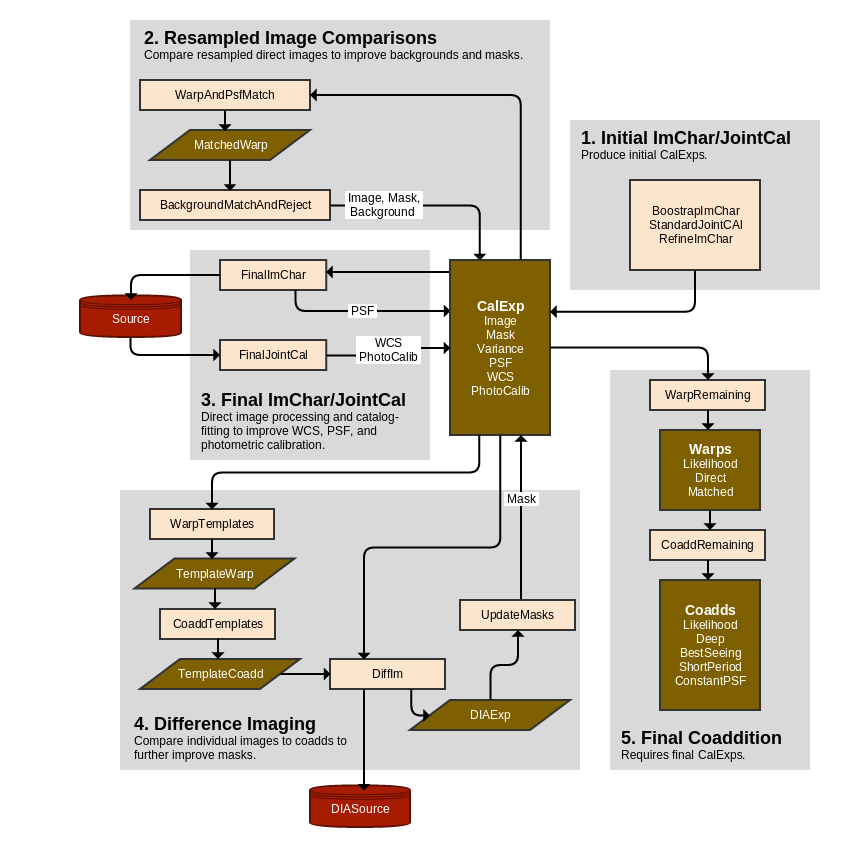
\includegraphics[width=\textwidth]{figures/drp_coaddition_and_diffim.png}
\caption{
  Data flow diagram for the Data Release Production coaddition and difference imaging pipelines.  Processing proceeds roughly counterclockwise, starting from the upper right with pipelines described in Section~\ref{sec:drp_imchar_and_jointcal}.  Each update to a component of the central CalExp dataset can in theory trigger another iteration of a previous loop, but in practice we will ``unroll'' these loops before production begins, yielding an acyclic graph with a series of incrementally updated CalExp datasets.  The nature of this unrolling and the number of iterations will be determined by future algorithmic research.  Numbered steps above are described more fully in the text.
  \label{fig:drp_coaddition_and_diffim}
}
\end{figure}

The processing flow in this pipeline group again centers around incremental updates to the CalExp dataset, which are limited here to its Background and Mask component (the Image component is also updated, but only to subract the updated background).  It will also return to the previous pipeline group described in Section~\ref{sec:drp_imchar_and_jointcal} to update other CalExp components.  The data flow between pipelines is shown in Figure~\ref{fig:drp_coaddition_and_diffim}, with the numbered steps are described further below:
\begin{enumerate} % note that the figure numbers aren't automatically linked
\item The first version of the CalExp dataset is produced by running the \hyperref[sec:drpBootstrapImChar]{BootstrapImChar}, \hyperref[sec:drpStandardJointCal]{StandardJointCal}, and \hyperref[sec:drpRefineImChar]{RefineImChar} pipelines, as described in Section~\ref{sec:drp_imchar_and_jointcal}.
\item We generate an updated Background and Mask via the \hyperref[sec:drpWarpAndPsfMatch]{WarpAndPsfMatch} and \hyperref[sec:drpBackgroundMatchAndReject]{BackgroundMatchAndReject} pipelines.  This produces the final CalExp Background and Image, and possibly the final Mask.
\item If the CalExp Mask has been finalized, we run the \hyperref[sec:drpFinalImChar]{FinalImChar} and \hyperref[sec:drpFinalJointCal]{FinalJointCal} pipelines.  These produce the final PSF, WCS, and PhotoCal.  If the Mask has not been finalized, we execute at least one iteration of the next step before this one.
\item We run the \hyperref[sec:drpWarpTemplates]{WarpTemplates}, \hyperref[sec:drpCoaddTemplates]{CoaddTemplates}, and \hyperref[sec:drpDiffIm]{DiffIm} pipelines to generate the DIASource and DIAExp datasets.  We may then be able to generate better CalExp Masks than we can obtain from \hyperref[sec:drpBackgroundMatchAndReject]{BackgroundMatchAndReject} by comparing the DIAExp masks across visits in the \hyperref[sec:drpUpdateMasks]{UpdateMasks} pipeline.
\item After all CalExp components have been finalized, we run the \hyperref[sec:drpWarpRemaining]{WarpRemaining} and \hyperref[sec:drpCoaddRemaining]{CoaddRemaining} to build additional coadd data products.
\end{enumerate}
The baseline ordering of these steps is thus \{1,2,3,4,5\}, but \{1,2,4,3,4,5\} is perhaps just as likely, and we may ultimately require an ordering that repeats steps 2 or 3.  Final decisions on the ordering and number of iteration will require testing with mature pipelines and a deep dataset taken with a realistic cadence; it is possible the configuration could even change between data releases as the survey increases in depth.  Fortunately, this reconfiguring should not require significant new algorithm development.

This pipeline group is responsible for producing the following final data products:
\begin{description}
\item[CalExp.\{Image,Background,Mask\}]  See above.
\item[DIAExp] A CCD-level \hyperref[sec:spImagesExposure]{Exposure} that is the difference between the CalExp and a template coadd, in the coordinate system and with the PSF of the CalExp.
\item[DIASource] A \hyperref[sec:spTablesSource]{SourceCatalog} containing sources detected and measured on the DIAExp images.
\item[ConstantPSFCoadd] A coadd data product (\hyperref[sec:spImagesExposure]{Exposure} or subclass thereof) with a constant, predefined PSF.
\item[DeepCoadd] A coadd data product built to optimize depth at the possible expense of seeing.
\item[BestSeeingCoadd] A coadd data product built to optimize image quality at the possible expense of depth.  Depending on the algorithm used, this may be the same as DeepCoadd.
\item[ShortPeriodCoadd] A coadd data product built from exposures in a short range of epochs, such as a year, rather than the full survey.
\item[LikelihoodCoadd] A coadd formed by correlating each image with its own PSF before combining them, used for detection and possibly building other coadds.
\item[ShortPeriodLikelihoodCoadd] Short-period likelihood coadds will also be built.
\item[TemplateCoadd] A coadd data product used for difference imaging in both DRP and AP, \emph{or} some other tract/patch/filter data product from which the template for a given airmass can be derived.
\end{description}

The nature of these coadd data products depends critically on whether we are able to develop efficient algorithms for optimal coaddition, and whether these coadds are suitable for difference imaging.  These algorithms are mathematically well-defined but computationally difficult; see \href{http://dmtn-015.lsst.io/en/latest/}{DMTN-15} for more information.  We will refer to the coadds produced by these algorithms as ``decorrelated coadds''; a variant with constant PSF (``constant-PSF partially decorrelated coadd'') is also possible.  This choice is also mixed with the question of how we will correct for differential chromatic refraction in difference imaging; some algorithms for DCR correction involve templates that are the result of inference on input exposures rather than coaddition.  There are five main scenarios for our use of decorrelated coadds:
\begin{description}
  \item[A] We use decorrelated coadds for all final coadd products.  DeepCoadd and ShortPeriodCoadd will be standard decorrelated coadds with a spatially-varying PSF, and ConstantPSFCoadd and TemplateCoadd will be constant-PSF partially-decorrelated coadds.  The BestSeeingCoadd data product will be dropped, as it will be redundant with DeepCoadd.  This will make coadds more expensive and complex to build, and require more algorithm development for coaddition, but will improve coadd-based measurements and make it easier to warm-start multi-epoch measurements.  Difference imaging may be easier, and more visits may be usable as inputs to templates due to softened or eliminated seeing cut.
  \item[B] We use decorrelated coadds for all coadds but TemplateCoadd.  Measurement is still improved, and the additional computational cost of coaddition is limited to a single pipeline that is not run iteratively.  Difference imaging may be harder, and the number of visits eligible for inclusion in templates may be reduced.  In this scenario, we still have two options for building templates:
  \begin{description}
    \item[B1] Templates will be built as PSF-matched coadds, or a product of PSF-matched coadds.
    \item[B2] Templates are the result of inference on resampled exposures with no PSF-matching.
  \end{description}
  \item[C] We do not use decorrelated coadds at all.  DeepCoadd, BestSeeingCoadd, and ShortPeriodCoadd will be direct coadds, and ConstantPSFCoadd will be a PSF-matched coadd.  Coaddition will be simpler and faster, but downstream algorithms may require more sophistication, coadd measurements may be lower quality, and multi-epoch measurements may be more difficult to optimize.  Here we again have the same two options for templates as option \textbf{B}:
  \begin{description}
    \item[C1] Templates will be built as PSF-matched coadds, or a product of PSF-matched coadds.
    \item[C2] Templates are the result of inference on resampled exposures with no PSF-matching.
  \end{description}
\end{description}
It is also possible to combine multiple scenarios across different bands.  In particular, we may not need special templates to handle DCR in redder bands, so we may select a simpler approach to dealing with them in those bands.  The final selection between these options will require experiments on LSST data or precursor data with similar DCR and seeing, though decorrelated coaddition algorithms and some approaches to DCR correction may be ruled out earlier if preliminary algorithm development does not go well.

Further differences in the pipelines themselves due to the presence or absence of decorrelated coadds will be described in the sections below.

\subsubsection{WarpAndPsfMatch}
\label{sec:drpWarpAndPsfMatch}

This pipeline resamples and then PSF-matches CalExp images from a visit into a single patch-level image with a constant PSF.  The resampling and PSF-matching can probably be accomplished separately by delegating to the \hyperref[sec:acWarping]{Image Warping} and \hyperref[sec:acPSFHomogenization]{PSF Homogenization} algorithmic components, respectively.  These operations can also be performed in the opposite order if the matched-to PSF is first transformed to the CalExp coordinate systems (so subsequent resampling yields a constant PSF in the coadd coordinate system).  Doing PSF-matching first may be necessary (or at least easier to implement) for undersampled images.

It is possible these operations will be performed simultaneously by a new algorithmic component; this could potentially yield improved computational performance and make it easier to properly track uncertainty.  These improvements are unlikely to be necessary for this pipeline, because these images and the coadds we build from them will only be used to estimate backgrounds and find artifacts, and these operations only require approximate handling of uncertainty.  However, other coaddition pipelines may require building an algorithmic component capable of warping and PSF-matching simultaneously, and if that happens, we would likely use it here as well.

The only output of the WarpAndPsfMatch pipeline is the MatchedWarp \hyperref[sec:spImagesExposure]{Exposure} intermediate data product.  It contains all of the usual \hyperref[sec:spImagesExposure]{Exposure} components, which must be propagated through the image operations as well.  There is a separate MatchedWarp for each \{patch, visit\} combination, and these can be produced by running WarpAndPsfMatch independently on each such combination.  However, individual CCD-level CalExps will be required by multiple patches, so I/O use or data transfer may be improved by running all WarpAndPsfMatch instances for a given visit together.

\subsubsection{BackgroundMatchAndReject}
\label{sec:drpBackgroundMatchAndReject}

This pipeline is responsible for generating our final estimates of the sky background and updating our artifact masks.  It is one of the most algorithmically uncertain algorithms in Data Release Production, particularly from the standpoint of large-scale data flow and parallelization, because while the algorithm is well-defined and understood for a small patch of sky, we do not yet have a concrete approach for extending it to large fields containing multiple dithered images (though it has been demonstrated on SDSS data, for which the drift-scan observation strategy makes the problem simpler).  It still processes tracts independently, but below that scale the parallelization is very much uncertain, and may in fact involve splitting these operations further into smaller pipelines.

The steps involved in background matching are described below.  All of these operations are performed on the MatchedWarp images; these are all in the same coordinate system and have the same PSF, so they can be meaningfully added and subtracted with no additional processing.
\begin{enumerate}
\item We define one of the visits that overlap an area of the sky as the \emph{reference image}.  At least in the naive local specification of the algorithm, this image must be smooth and continous over the region of interest.  This is done by the \hyperref[sec:acBuildBackgroundReference]{Build Background Reference} pipeline, which must artificially (but reversibly) enforce continuity in a reference image that stitches together multiple visits to form a single-epoch-deep full tract image, unless we develop an approach for dealing with discontinuity downstream.
\item We subtract the reference image from every other visit image.  This must account for any artifical features due to the construction of the reference image.
\item We run \hyperref[sec:acSourceDetection]{Source Detection} on the per-visit difference images to find artifacts and transient sources.  We do not generate a traditional catalog of these detections, as they will only be used to generate improved CalExp masks; they will likely be stored as a sequence of \hyperref[sec:spFootprints]{Footprints}.
\item We estimate the background on the per-visit difference images by delegating to the \hyperref[sec:acBackgroundEstimation]{Background Estimation} algorithmic component.  This difference background should be easier to be model than a direct image background, as the image will be mostly free of sources and astrophysical backgrounds.
\item We build a PSF-matched coadd by adding all of the visit images (including the reference) and subtracting all of the difference image backgrounds; this yields a coadd that contains only the reference image background, which we then model and subtract by again using the \hyperref[sec:acBackgroundEstimation]{Background Estimation} algorithmic component.  Combining the images will be performed by the \hyperref[sec:acCoaddition]{Coaddition} algorithmic component, which will also generate new CalExp masks by analyzing the per-pixel, multi-visit histograms of image and mask values (e.g. generalized statistical outlier rejection) to distinguish transients and artifacts from variable sources.
\end{enumerate}

We are assuming in the baseline plan that we can use a matched-to PSF in \hyperref[sec:drpWarpAndPsfMatch]{WarpAndPsfMatch} large enough to match all visit images to it without deconvolution.  If a large marged-to PSF adversely affects subsequent processing in \hyperref[sec:drpBackgroundMatchAndReject]{BackgroundMatchAndReject}, we may need to develop an iterative approach in which we apply \hyperref[sec:drpWarpAndPsfMatch]{WarpAndPsfMatch} only to better-seeing visits first, using a smaller target PSF, run \hyperref[sec:drpBackgroundMatchAndReject]{BackgroundMatchAndReject} on these, and then re-match everything to a larger target PSF and repeat with a larger set of input visits.  However, this problem would suggest that the \hyperref[sec:drpDiffIm]{DiffIm} and \hyperref[sec:drpUpdateMasks]{UpdateMasks} pipelines would be even better at finding artifacts, so a more likely mitigation strategy would be to simply defer final Mask generation to after at least one iteration of those pipelines, as described in the discussion of Figure~\ref{fig:drp_coaddition_and_diffim} at the beginning of Section~\ref{sec:drp_coaddition_and_diffim}.

The outputs of BackgroundMarchAndReject are updated Background and Mask components for the CalExp product.  Because it is not built with the final photometric and astrometric calibration, the PSF-matched coadd built here is discarded.

\subsubsection{WarpTemplates}
\label{sec:drpWarpTemplates}

This pipeline is responsible for generating the resampled visit-level images (TemplateWarp) used to build template coadds for difference imaging.  The algorithmic content of this pipeline and the nature of its outputs depends on whether we are using decorrelated coadds (option \textbf{A}) at the beginning of \ref{sec:drp_coaddition_and_diffim}), PSF-matched coadds (\textbf{B1} or \textbf{C1}), or inferring templates (\textbf{B2} or \textbf{C2}).

If we are using decorrelated coadds (option \textbf{A}), the output is equivalent to the LikelihoodWarp data product produced by the \hyperref[sec:drpWarpRemaining]{WarpRemaining} pipeline (aside from differences due to the state of the input CalExps), and the algorithm to produce it the same:
\begin{itemize}
\item We correlate the image with its own PSF by delegating to the \hyperref[sec:spKernels]{Convolution Kernels} software primitive.
\item We resample the image by delegating to the \hyperref[sec:acWarping]{Image Warping} algorithmic component.
\end{itemize}
As with other convolution-and-warping pipelines, it is possible we will instead develop a single algorithmic component to perform both operations.  These operations must include full propogation of uncertainty.

If we are not using decorrelated coadds (\textbf{B1} or \textbf{C1}), the output is equivalent to the MatchedWarp data product, and the algorithm is the same as the \hyperref[sec:drpWarpAndPsfMatch]{WarpAndPsfMatch} pipeline that produces.  We cannot reuse existing MatchedWarps simply because we need to utilize updated CalExps.

If we are inferring templates (\textbf{B2} or \textbf{C2}), this pipeline is only responsible for resampling, producing an output equivalent to the DirectWarp data product produced by the \hyperref[sec:drpWarpRemaining]{WarpRemaining} pipeline.  This work is delegated to the \hyperref[sec:acWarping]{Image Warping} algorithmic component.

\subsubsection{CoaddTemplates}
\label{sec:drpCoaddTemplates}

This pipeline generates the TemplateCoadd dataset used as the reference image for difference imaging.  This may not be a simple coadd, at least in bluer bands; in order to correct for differential chromatic refraction during difference imaging, we may need to add a wavelength or airmass dimension to the usual 2-d image, making a 3-d dimensional quantity.  The size of the third dimension will likely be small, however, so it should be safe to generally consider TemplateCoadd to be a small suite of coadds, in which a 2-d image is the result a different sum of or fit to the usual visit-level images (the TemplateWarp dataset, in this case).

Most of the work is done by the \hyperref[sec:acDCRTemplates]{DCR-Corrected Template Generation} algorithmic component, but its behavior depends on which of the coaddition scenarios is selected from the list at the beginning of Section~\ref{sec:drp_coaddition_and_diffim}):
\begin{description}
\item[A,B1,C1] One or more coadd-like images (corresponding to different wavelengths, airmasses, etc.) are created by delegating to the \hyperref[sec:acCoaddition]{Coaddition} algorithmic component to sum the TemplateWarp images with different weights.  \textbf{A only:} coadded images are then partially decorrelated to constant PSF by delegating to the \hyperref[sec:acCoaddDecorrelation]{Coadd Decorrelation} algorithmic component.
\item[B2,C2] The template is inferred from the resample visit images using an inverse algorithm that is yet to be developed.
\end{description}

\subsubsection{DiffIm}
\label{sec:drpDiffIm}

In the DiffIm pipeline, we subtract a warped TemplateCoadd from each CalExp, yielding the DIAExp image, where we detect and characterize DIASources.  This is quite similar to Alert Production's \hyperref[sec:apAlertDetection]{Alert Detection} pipeline but may not be identical for several reasons.  The AP variant must be optimized for low latency, and hence may avoid full-visit processing that is perfectly acceptable in DRP.  In addition, the input CalExps will have been better characterized in DRP, which may make some steps taken in AP unimportant or even counterproductive.  However, we expect that the algorithmic components utilized in DRP are the same as those used by AP.

The steps taken by DRP DiffIm are:
\begin{enumerate}
\item Retrieve the DiffIm template appropriate for the CalExps to be processed (probably handling a full visit at a time), delegating to the \hyperref[sec:acRetrieveTemplate]{Template Retrieval} algorithmic component.  This selects the appropriate region of sky, and if necessary, collapses a higher-dimensional template dataset to a 2-d image appropriate for the CalExp's airmass.
\item (optional) Correlate the CalExp with its own PSF, delegating to the \hyperref[sec:spKernels]{Convolution Kernel} software primitive.  This is the ``preconvolution'' approach to difference imaging, which makes PSF matching easier by performing PSF-correlation for detection first, reducing or eliminating the need for deconvolution.  This approach is theoretically quite promising but still needs development.
\item Resample the template to the coordinate system of the CalExp, by delegating to the \hyperref[sec:acWarping]{Image Warping} algorithmic component.
\item Match the template's PSF to the CalExp's PSF and subtract them, by delegating to the \hyperref[sec:acImageSubtraction]{Image Subtraction} algorithmic component.
\item Run \hyperref[sec:acSourceDetection]{Source Detection} on the difference image.  We correlate the image with its PSF first using the \hyperref[sec:spKernels]{Convolution Kernels} software primitive unless this was done prior to subtraction.
\item (optional) Decorrelate the CalExp by delegating to the \hyperref[sec:acDiffImDecorrelation]{Difference Image Decorrelation} algorithmic component.
\item Run \hyperref[sec:acDiffImMeasurement]{DiffIm Measurement} on the difference image to characterize difference sources.  If preconvolution is used but decorrelation is not, the difference image cannot be measured using algorithms applied to standard images; alternate algorithms may be developed for some measurements, but perhaps not all.
\end{enumerate}

DiffIm can probably be run entirely independently on each CCD image; this will almost certainly be taken in Alert Production.  However, joint processing across a full visit may be more computationally efficient for at least some parts of template retrieval, and PSF-matching may produce better results if a more sophisticated full-visit matching algorithm is developed.

\subsubsection{UpdateMasks}
\label{sec:drpUpdateMasks}

UpdateMasks is an optional pipeline that is only run if DIAExp masks are being used to update CalExp masks.  As such, it is not run after the last iteration of \hyperref[sec:drpDiffIm]{DiffIm}, and is never run if \hyperref[sec:drpBackgroundMatchAndReject]{BackgroundMatchAndReject} constructs the final CalExp masks.

Like \hyperref[sec:drpBackgroundMatchAndReject]{BackgroundMatchAndReject}, UpdateMasks compares the histogram of mask values at a particular spatial point to determine which masks correspond to transients (both astrophysical sources and artifacts; we want to reject both from coadds) and which correspond to variable objects.  This work is delegated to \hyperref[sec:acCoaddition]{Coaddition}.

\subsubsection{WarpRemaining}
\label{sec:drpWarpRemaining}

This pipeline is responsible for the full suite of resampled images used to build coadds in \hyperref[sec:drpCoaddRemaining]{CoaddRemaining}, after all CalExp components have been finalized.  It produces some combination of the following data products, depending on the scenario(s) described at the beginning of Section~\ref{sec:drp_coaddition_and_diffim}:
\begin{description}
\item[LikelihoodWarp] CalExp images are correlated with their own PSF, then resampled, via the \hyperref[sec:spKernels]{Convolution Kernels} software primitive and the \hyperref[sec:acWarping]{Image Warping} algorithmic component.  LikelihoodWarp is computed in all scenarios, but in option \textbf{C} it may not need to propogate uncertainty beyond the variance, as the resulting coadd will be used only for detection.
\item[MatchedWarp] As in \hyperref[sec:drpWarpAndPsfMatch]{WarpAndPsfMatch}, CalExp images are resampled then matched to a common PSF, using \hyperref[sec:acWarping]{Image Warping} and \hyperref[sec:acPSFHomogenization]{PSF Homogenization}.  MatchWarp is only produced in option \textbf{C}.
\item[DirectWarp] CalExp images are simply resampled, with no further processing of the PSF, using \hyperref[sec:acWarping]{Image Warping}.  MatchWarp is only produced in option \textbf{C}.
\end{description}

Given that all of these steps involve resampling the image, it would be desirable to do the resampling once up front, and then proceed with the PSF processing.  While this is mathematically possible for all of these cases, it would signficantly complicate the PSF correlation step required for building LikelihoodWarps.

\subsubsection{CoaddRemaining}
\label{sec:drpCoaddRemaining}

In CoaddRemaining, we build the suite of coadds used for deep detection, deblending, and object characterization.  This includes the Likelihood, ShortPeriodLikelihood, Deep, BestSeeing, ShortPeriod, and ConstantPSF Coadds.

The algorithms again depend on the scenarios outlined at the beginning of Section~\ref{sec:drp_coaddition_and_diffim}:
\begin{description}
\item[A,B] All non-template coadds are built from LikelihoodWarps.  We start by building ShortPeriodLikelihoodCoadds by simple coaddition of the LikelihoodWarps, using the \hyperref[sec:acCoaddition]{Image Coaddition} algorithmic component.  We decorrelate these using the \hyperref[sec:acCoaddDecorrelation]{Coadd Decorrelation} algorithmic component to produce ShortPeriodCoadds, then sum the ShortPeriodLikelihoodCoadds to produce the full LikelihoodCoadd.  The full LikelihoodCoadd is then decorrelated to produce DeepCoadd and ConstantPSFCoadd.
\item[C] We generate LikelihoodCoadd and ShortPeriodLikelihoodCoadds using the same approach as above (though the accuracy requirements for uncertainty propagation are eased). ShortPeriodCoadd, DeepCoadd, and BestSeeingCoadd are then built as different combinations of DirectWarp images, again using the \hyperref[sec:acCoaddition]{Image Coaddition} algorithmic component.  ConstantPSFCoadds are built by combining MatchedWarps.
\end{description}

\subsection{Coadd Processing}
\label{sec:drp_coadd_processing}

In comparison to the previous two pipeline groups, coadd processing is relatively simple.  All pipelines operate on individual patches, and there is no large-scale iteration between pipelines.  These pipelines may individually require complex parallelization at a lower level, as they will frequently have memory usage above what can be expected to fit on a single core.

\subsubsection{DeepDetect}
\label{sec:drpDeepDetect}

This pipeline simply runs the \hyperref[sec:acSourceDetection]{Source Detection} algorithmic component on combinations of LikelihoodCoadds and ShortPeriodLikelihoodCoadds, then optionally performs additional preliminary characterization on related coadds.  These combinations are optimized for detecting objects with different SEDs, and there are a few different scenarios for what combinations we'll produce (which are not mutually exclusive):
\begin{itemize}
\item We could simply detect on each per-band LikelihoodCoadds separately.
\item We could build a small suite of cross-band LikelihoodCoadds corresponding to simple and artificial but approximately spanning SEDs (flat spectrums, step functions, etc.).
\item We could build a large suite of cross-band LikelihoodCoadds corresponding to a library of real star, galaxy, and QSO SEDs.
\item We could build a single $\chi^2$ coadd, which is only optimal for objects the color of the sky, but may be close enough to optimal to detect a broad range of SEDs.
\end{itemize}
Any of these combinations may also be used to combine ShortPeriodLikelihoodCoadds.

We may also convolve the images further or bin them to improve our detection efficiency for extended objects.

Actual detection on these images may be done with a lower threshold than our final target threshold of 5$\sigma$, to account for loss of efficiency due using the incorrect SED or morphological filter.

The details of the suite of detection images and morphological filters is a subject requiring further algorithmic research on precursor data (or LSST/ComCam data) at full LSST depths with at least approximately the right filter set.

After detection, CoaddSources may be deblended and characterized by running the \hyperref[sec:acSingleFrameDeblending]{Single Frame Deblending}, \hyperref[sec:acSingleFrameMeasurement]{Single Frame Measurement}, and \hyperref[sec:acSingleFrameClassification]{Single Frame Classification} algorithmic components on DeepCoadd and ShortPeriodCoadd combinations that correspond to the LikelihoodCoadd combinations used for detection.  These characterizations (like the rest of the CoaddSource tables) will be discarded after the \hyperref[sec:drpDeepAssociate]{DeepAssociate} pipeline is run, but may be necessary to inform higher-level association algorithms run there.  The requirements on characterization processing in this pipeline will be set by the needs of the \hyperref[sec:drpDeepAssociate]{DeepAssociate} pipeline, but we do not expect it to involve significant new code beyond what will be used by the various ImChar pipelines.

The only output of DeepDetect is the suite of CoaddSource tables (one for each detection image) containing \hyperref[sec:spFootprints]{Footprints}, peaks, and characterizations necessary for association.

\subsubsection{DeepAssociate}
\label{sec:drpDeepAssociate}

In DeepAssociate, we perform a sophisticated spatial match of all CoaddSources and DIASources, generating tables of DIAObjects, Object candidates, and SSObject detections.  We do \emph{not} include the Source table in this merge, as virtually all Sources correspond to astrophysical objects better detected in \hyperref[sec:drpDeepDetect]{DeepDetect} or \hyperref[sec:drpDiffIm]{DiffIm}.

The baseline plan for association is to first associate DIASources into DIAObjects using the same approach used in Alert Production (i.e. the \hyperref[sec:acDIAObjectGeneration]{DIAObject Generation} algorithmic component), then associate DIAObjects with the multiple CoaddSource tables (using the \hyperref[sec:acObjectGeneration]{Object Generation} algorithmic component).  DIASources not associated into DIAObjects will be considered candidates for merging SSObjects, which will happen in the \hyperref[sec:drpMOPS]{MOPS} pipeline.

These association steps must be considerably more sophisticated than simple spatial matching; they must utilize the limited flux and classification information available from detection to decide whether to merge sources detected in different contexts.  This will require astrophysical models to be included in the matching algorithms at some level; for instance:
\begin{itemize}
\item We must be able to associate the multiple detections that correspond to high proper-motion stars into a single Object.
\item We must not associate supernovae with their host galaxies, despite the fact that their positions may be essentially the same.
\end{itemize}
To meet these goals (as well as similar ones which still need to be specififed), DeepAssociate will have to generate \emph{multiple} hypotheses for some blend families.  Some of these conflicting hypotheses will be rejected by the \hyperref[sec:drpDeepDeblend]{DeepDeblend}, while others may be present in the final Object catalog (flags will be used to indicate different interpretations and our most likely interpretation).  This is a generalization of the simple parent/child hierarchy used to describe different blend hypotheses in the SDSS database (see Section~\ref{sec:introDataUnits}).

It is possible that associations could be improved by doing both merge steps simultaneously (under the hypothesis that CoaddSource presence or absence could be used to improve DIASource association).  This is considered a fallback option if the two-stage association procedure described above cannot be made to work adequately.

The output of the DeepAssociate pipeline is the first version of the Object table, containing a superset of all Objects that will be characterized in later pipelines.

\subsubsection{DeepDeblend}
\label{sec:drpDeepDeblend}

This pipeline simply delegates to the \hyperref[sec:acMultiCoaddDeblending]{Multi-Coadd Deblending} algorithmic component to deblend all Objects in a particular patch, utilizing all non-likelihood coadds of that patch.  This yields \hyperref[sec:spFootprints]{HeavyFootprints} containing consistent deblended pixels for every object in every (non-likelihood) coadd, while rejecting as many deblend hypotheses as possible to reduce the number of hypotheses that must be subsequently measured.

While the pipeline-level code and data flow is simple, the algorithmic component is not.  Not only must deblending deal with arbirarily complex superpositions of objects with unknown morphologies, it must do so consistently across bands and the epoch ranges (with different PSFs) and ensure proper handling of Objects spawned by DIASources that may not even appear in coadds.  It must also parallelize this work efficiently over multiple cores; in order to fit patch-level images for all coadds in memory, the processing of at least the largest individual blend families must themselves be parallelized.  This may be done by splitting the largest blend families into smaller groups that can be processed in parallel with only a small amount of serial iteration; it may also be done by using low-level multithreading over pixels.

The output of the DeepDeblend pipeline an update to the Object table, which adds columns (mostly flags) and removes some rows from the table produced by DeepAssociate.

\subsubsection{MeasureCoadds}
\label{sec:drpMeasureCoadds}

The MeasureCoadds pipeline delegates to the \hyperref[sec:acMultiCoaddMeasurement]{Multi-Coadd Measurement} algorithmic component to jointly measure all Objects on all coadds in a patch.

Like \hyperref[sec:drpDeepDeblend]{DeepDeblend}, this pipeline is itself quite simple, but it delegates to a complex algorithmic component (but a simpler one than \hyperref[sec:acMultiCoaddDeblending]{Multi-Coadd Deblending}).  There are three classes of open questions in how multi-coadd measurement will proceed:
\begin{itemize}
\item What parameters will be fit jointly across bands, and which will be fit independently?  The measurement framework for multi-coadd measurement is designed to support joint fitting, but it is likely that some algorithms will simply be \hyperref[sec:acSingleFrameMeasurement]{Single Frame Measurement} or \hyperref[sec:acForcedMeasurement]{Forced Measurement} plugins that are simply run independently on the DeepCoadd and/or ConstantPSFCoadd in each band.  Making these decisions will require experimentation on deep precursor and simulated data.
\item How will we measure blended objects?  Coadd measurement will at least begin by using the \hyperref[sec:spFootprints]{HeavyFootprints} produced by \hyperref[sec:drpDeepDeblend]{DeepDeblend} to use the \hyperref[sec:acReplaceNeighborsWithNoise]{Neighbor Noise Replacement} approach, but we may then use \hyperref[sec:acSimultaneousFitting]{Simultaneous Fitting} to generate improved warm-start parameters for \hyperref[sec:drpMultiFit]{MultiFit} or to build models we can use as PSF-deconvolved templates to enable the \hyperref[sec:acDeblendTemplateProjection]{Deblend Template Projection} approach in \hyperref[sec:drpMultiFit]{MultiFit} and/or \hyperref[sec:drpForcedPhotometry]{ForcedPhotometry}.
\item How will we parallelize?  As with \hyperref[sec:drpDeepDeblend]{DeepDeblend}, keeping the full suite of coadds in memory will require processing at least some blend families using many cores.  For algorithms that don't require joint fitting across different coadds, this could be done by measuring each coadd independently in parallel, but the most expensive algorithms (e.g. galaxy model fitting) are likely to be the ones where we'll want to fit jointly across bands.
\end{itemize}

The output of the MeasureCoadds pipeline is an update to the Object table, which adds columns containing measured quantities.

\subsection{Overlap Resolution}
\label{sec:drp_overlap_resolution}

The two overlap resolution pipelines are together responsible for finalizing the definitions of Objects by merging redundant processing done in tract and patch overlap regions.  In most cases, object definitions in the overlap region will be the same, making the problem trivial, and even when the definitions are different we can frequently resolve the problem using purely geometrical arguments.  However, some difficult cases will remain, mostly relating to blend families that are defined differently on either side.

We currently assume that overlap resolution actually drops Object rows when it merges them; this will avoid redundant processing in the performance critical \hyperref[sec:drpMultiFit]{MultiFit} pipeline.  A slower but perhaps safer alternative would be to simply flag redundant Objects.  This would also allow tract overlap resolution to be moved after the \hyperref[sec:drpMultiFit]{MultiFit} and \hyperref[sec:drpForcedPhotometry]{ForcedPhotometry} pipelines, which would simplify large-scale parallelization and data flow by moving the first operation requiring more than one tract (\hyperref[sec:drpResolveTractOverlaps]{ResolveTractOverlaps} until after all image processing is complete.

\subsubsection{ResolvePatchOverlaps}
\label{sec:drpResolvePatchOverlaps}

In patch overlap resolution, all contributing patches to an area (there can be between one and four) share the same pixel grid, and we furthermore expect that they will have the same coadd pixel values.  This should ensure that any above-threshold pixel in one patch is also above threshold in all others, which in turn should guarantee that patches agree on the extent of each blend family (as defined by the parent \hyperref[sec:spFootprints]{Footprint}).

A common pixel grid also allows us to define the overlap areas as exact rectangular regions; we consider each patch to have an inner region (which directly abuts the inner regions of neighboring patches) and an outer region (which extends into the inner regions of neighboring patches).  If we consider the case of two overlapping patches, blend families in those patches can fall into five different categories:
\begin{itemize}
\item If the family falls strictly within one patch's inner region, it is assigned to that patch (and the other patch's version of the family is dropped).
\item If the family crosses the boundary between patch inner regions...
  \begin{itemize}
  \item ...but is strictly within both patches' outer regions, it is assigned to the patch whose inner region includes more of the family's footprint area.
  \item ...but is strictly within only one patch's outer region, it is assigned to that patch.
  \item ...and is not strictly within either patch's outer region, the two families must be merged at an Object-by-Object level.  The algorithm used for this procedure is yet to be developed, but will be implemented by the \hyperref[sec:acBlendedOverlapResolution]{Blended Overlap Resolution} algorithmic component.
  \end{itemize}
\end{itemize}
Overlap regions with more than two patches contributing have more possibilities, but are qualitatively no different.

\begin{note}[TODO]
  Add figure explaining inner and outer patch regions.
\end{note}

If pixel values in patch overlap regions cannot be guaranteed to be identical, patch overlap resolution becomes significantly harder (but no harder than tract overlap resolution), because adjacent patches may disagree on the above categories to which a family belongs.

Patch overlap resolution can be run independently on every distinct overlap region that has a different set of patches contributing to it; in the limit of many patches per tract, there are three times as many overlap regions as patches (each patch has four overlap regions shared by two patches, and four overlap regions each shared by four patches).

\subsubsection{ResolveTractOverlaps}
\label{sec:drpResolveTractOverlaps}

Tract overlap resolution operates under the same principles as patch overlap resolution, but the fact that different tracts have different coordinate systems and subtly different pixel values makes the problem significantly more complex.

While we do not attempt to define inner and outer regions for tracts, we can still define discrete overlap regions in which the set of contributing tracts is constant (though these regions must now be defined using spherical geometry).  Because tracts may differ on the extent and membership of blend families, it will be useful here to define the concept of a ``blend chain'': within an overlap region a families blend chain is the recursive union of all families it overlaps with in any tract that contributes to that overlap region see Figure~TODO.  A blend chain is thus the maximal cross-tract definition of the extent of a blend family, and hence we can use it to categorize blends in tract overlaps:
\begin{itemize}
\item If a blend chain is strictly contained by only one tract, all families within that chain are assigned to that tract.
\item If a blend chain is strictly contained by more than one tract, all families within that chain are assigned to the tract whose center is closest to the centroid of the blend chain.
\item If a blend chain is not strictly contained by any tract, all families in the chain must be merged at an Object-by-Object level.  This is done by the \hyperref[sec:acBlendedOverlapResolution]{Blended Overlap Resolution} algorithmic component, after first transforming all measurements to a new coordinate system defined to minimize distortion due to projection (such as a tangent projection at the blend chain's centroid).
\end{itemize}

ResolveTractOverlaps is the first pipeline in Data Release Production to require access to processed results from more than one tract.

\begin{note}[TODO]
  Add figure explaining blend chains.
\end{note}

\subsection{Multi-Epoch Object Characterization}
\label{sec:drp_multi_epoch_object_characterization}

\begin{note}[Object Characterization Diagram]
Extract multifit/forced\_photometry pipelines from ``DRP Top-Level Overview'' on confluence and expand detail to show data flow and ordering of ``Task/Process'' boxes.
\end{note}

\subsubsection{MultiFit}
\label{sec:drpMultiFit}

\subsubsection{ForcedPhotometry}
\label{sec:drpForcedPhotometry}

\subsection{Postprocessing}
\label{sec:drp_postprocessing}

\begin{note}[Postprocessing Diagram]
Extract Afterburner pipelines from ``DRP Top-Level Overview'' on confluence and expand detail to show data flow and ordering of ``Task/Process'' boxes.
\end{note}

\subsubsection{MOPS}
\label{sec:drpMOPS}
\subsubsection{MakeSelectionMaps}
\label{sec:drpMakeSelectionMaps}
\subsubsection{Classification}
\label{sec:drpClassification}
\subsubsection{GatherContributed}
\label{sec:drpGatherContributed}

\subsection{UNSTRUCTURED OPEN QUESTIONS}

\begin{itemize}
\item Where does the initial reference catalog at the start of the DRP come from?  This could require special observations in commissioning or before the start of the survey, as well as addition algorithms and software.  If DRP always uses a reference catalog for star selection in ImChar, we need to actually do the classification for that at some point.
\item How do we test all of the wavelength-dependent photometric calibration and PSF stuff on precursor data?  Are we going to characterize DECam well enough to just use it directly, or do we need to mock things up or rely more on JointCal?
\item Input selection for DRP.  How do we decide what to throw away?  Is this a SQuaRE job?  Do we ever throw images away because the pipeline can't process them?  Do we report these back to the scheduler, or just hope it all averages out?
\item Shouldn't we be making difference images from short-period coadds, instead of using the short-period coadds directly?
\item Do we need to resolve tract overlaps in Source and DIASource as well?
\end{itemize}



\section{Science Data Quality Assurance (SDQA)}
\label{sec:sdqa}

\subsection{Overview of SDQA}

Science Data Quality Assurance (SDQA) describes a collection of
capabilities for Quality Analysis (QA) and Quality Control (QC) that
collectively ensure a high quality performing software system as well
as the ability to meet the scientific goals of the system. These are
designed to service LSST's quality assessment needs through all phases
of Construction, Commissioning and Operations. Consumers of these
services may include developers, facility staff, DAC (e.g., Level 3)
users, and the general LSST science user community.

SDQA capabilities can be divided into Quality Analysis (QA) and
Quality Control (QC) Capabilities.

\subsubsection{Quality Analysis (QA)}

Quality Analysis describes a range of \emph{activities} aimed at understanding the algorithmic performance of the code and eventually the properties of the data. These are achieved by a set of \emph{tools} that leverage components of the Data Management subsystem, as well as additional capabilities as necessary, to allow for the scientific inspection of data both by DM developers and scientists during construction as well as commissioning engineers and scientists during commissioning and operations.

QA activities include processing, analysing and inspecting data for forensic purposes. They also include the development of tests for verifying and characterising algorithmic performance, and are closely tied to the development of the Science Pipelines and the Science User Interface.

\subsubsection{Quality Control (QC)}

Quality Control describes a range of \emph{services and processes} aimed at measuring and monitoring and characterising the system (both software and data) to verify and characterise its performance. Whereas Quality Assurance describes the activities of people, Quality Control describes systems running autonomously and only notify people when an anomaly that cannot be automatically rectified is detected.

QC services include regression detection, measurement of Key Performance Metrics, a notification infrastructure and quality monitor dashboards. They are primarily the responsibility of the Science Quality and Reliability Engineering (SQuaRE) team.

\subsection{Key Features of SDQA (QA and QC) systems}

\begin{itemize}
\item SDQA provides capabilities for science data quality analysis of Level 1, 2, and Calibration Processing pipelines.

\item SDQA provides services to support software development in Construction, Commissioning and Operations.

\item SDQA provides for the visualization, analysis and monitoring capabilities needed for common science quality data analysis use cases. Its inputs may be gathered from SDQA services, the production pipelines, engineering data sources and non-LSST data sources.

\item SDQA has the flexibility to support execution of ad-hoc (user-driven) tests and analyses of ad-hoc datasets (provided they are supported by the LSST stack) within a standard framework.

\item SDQA supports use cases involving interactive ``drill-down'' of QC data exposed through its visualization interfaces.

\item SDQA allows for notifications to be issued when monitoring quantities that fall outside permissible bounds and/or have degraded over historical values.

\item SDQA is able to collect and harvest the outputs and logs of execution of a pipeline, and extract and expose metrics from these logs.

\item SQDA makes provision to store outputs that are not stored through other LSST data access services.

\item SDQA is deployable as high-reliability scalable services for production as well as allow for core data assessment functionality to be executed on a developer's local machine.

\item SDQA is architected in a manner that would enable it to be deployable on standard cloud architectures outside of the LSST facilities so that community-based L3 development activities can be supported.

\end{itemize}

\subsection{Key Tasks for Each Tier of QC}

SDQA system provides a framework that is capable of monitoring QC information at four different stages of capability and maturity:

\begin{itemize}
\item[QA Tier 0] Testing and Validation of the DM sub-system during software development
\item[QA Tier 1] Real-time data quality and system assesment during commissioning and operations (also, forensics)
\item[QA Tier 2] Quality assessment of Data Releases (also, forensics)
\item[QA Tier 3] Ability for the community to evaluate the data quality of their own analyses. These should made available as well-documented and deployable versions of core QC Tier 0--2 services.
\end{itemize}

A view of the tiered QC services is shown in \ref{fig:qa-overview}. Capabilities are increasingly layered (eg. tier QC-1 includes QC-0 services). A definition of the QC tiers is given in the rest of this section.

\begin{figure}
\centering
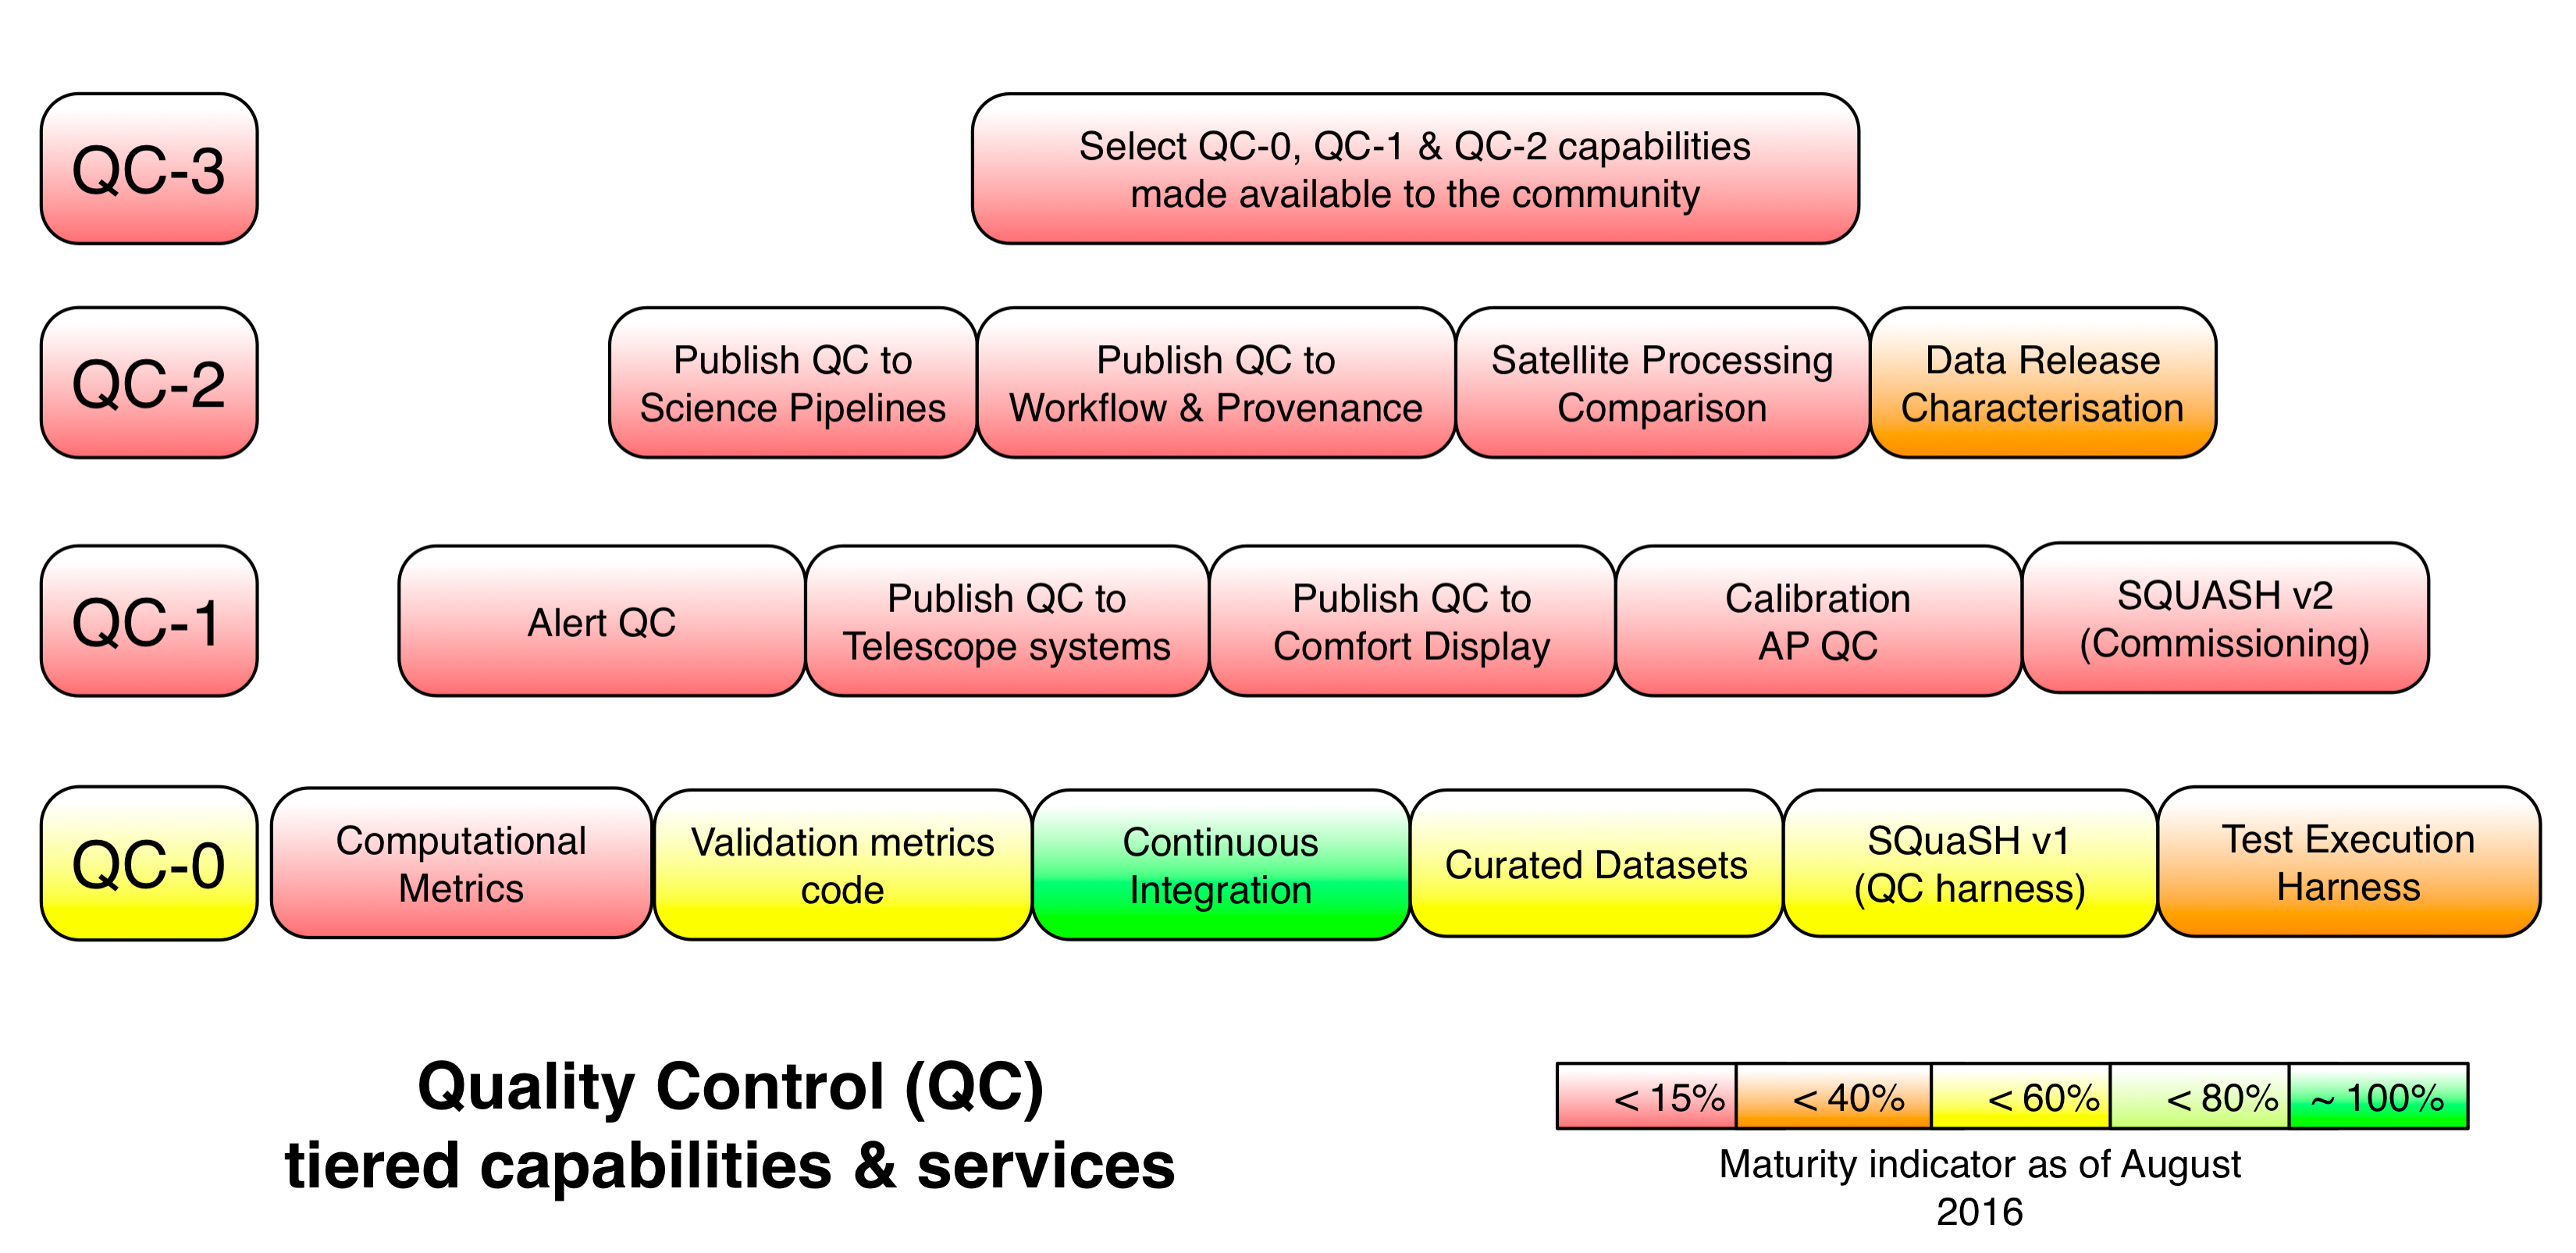
\includegraphics[width=\textwidth]{figures/qa_services.png}
\caption{Layer of progressive QC capabilities across all 4 tiers of QC.
\label{fig:qa-overview}}
\end{figure}



\subsubsection{QA Tier 0}

The first step to good quality data is good quality software. The purpose of QC-0 services is to enable testing of the DM software during development as well as validate software improvements during commissioning and operations, quantifying the software performance against known and/or expected inputs and outputs.

The core capabilities of QC-0 services are:

\paragraph{Continuous Integration Services}
\label{sec:qaCI}
\begin{itemize}

\item Continuous integration services compile code to uncover build errors and to trap failures in unit tests.

\item Builds of references (tags, branches) that can happen on a schedule, on developer request or on development events (e.g.,  merge to master)

\item SDQA provides CI services on multiple reference platforms and uses OS and compiler portability testing as a way to ensure the codebase is well engineered for future use.

\end{itemize}

\paragraph{Test Execution Harness}
\label{sec:qaTestharness}
\begin{itemize}

\item A test execution harness runs tests (such as data analysis unit
  tests) on a regular cadence (e.g.\ nightly/weekly/monthly) to allow
  basic functional checkout of the code. Tests written as part of Tier
  1-3 QC can be added directly by developers and be caused to execute
  without manual intervention, for example by checking in code or a
  specification in a purpose built test repository.

\item The test execution harness also allows the selection of a number of appropriate reference datasets (see \ref{sec:qaCurateddata}

\item Results from such tests are exposed in such a way as to allow summary reports and meaningful failure notifications.

\end{itemize}

\paragraph{Verification Metrics Code}
\label{sec:qaVerify}
\begin{itemize}

\item During Construction, progress towards meeting DM subsystem requirements revolve around the Key Performance Metrics (KPMs) outlined in LDM-240. SDQA implements code to calculate these KPMs. Consult \emph{reference to KPM Verification document} for a list of those metrics and how (and by whom and on what) they will be calculated.

\item Additional metrics must be calculated to be met in order for the DM subsystem to demonstrate its operational readiness. The list of those metrics and how (and by whom) they will be calculated will be in \emph{reference to DM Verification Plan CoDR document}. In terms of QC infrastructure, these metrics will not require different capabilities than the KPMs.

\item Verification code will be implemented in such a way that it can run with normal pipeline processing on developer's laptops, either inline or as after-burners as appropriate.

\item Additional metrics may be proposed during construction that are helpful to development or algorithm characterisation, either by developers investigating algorithms or as part of characterising the complete scientific and computational performance of the DM subsystem. SDQA will provide ways of executing that code in a similar way to KPMs, but apps developers may need to contribute the code (or at least document the algorithmic approach) to calculate those metrics.

\end{itemize}

\paragraph{Computational Metrics}
\label{sec:qaComputational}
\begin{itemize}

\item While the scope of this document is the scientific aspects of the pipelines, SDQA must also accommodate non-scientific KPMs and other metrics, such as computational performance characterisation.

\item SDQA will provide a capability to instrument the production pipelines to calculate computational performance metrics, and harvest data from those instrumentations (via logs or more direct ways of populating the QC database tables).

\item The computational performance metrics that SDQA calculates will be in practice surrogates for the actual computational performance in production since those will depend on the production system architecture. The purpose of calculating those as part of SDQA is to continuously monitor relative performance to alert the developers that a regression has occurred.

\item SDQA can calculate modeled system performance from the surrogate computational metrics if a model is provided to it (e.g., from Architecture).

\item A library of these instrumentations will be provided so that they can be mixed and matched to pipelines depending on the performance metric of interest.

\end{itemize}

\paragraph{Curated Datasets}
\label{sec:qaCurateddata}
\begin{itemize}

\item Part of the process for validating the software and its performance is selecting rich but targeted standardized data sets to generate directly comparable metrics between different versions of the software.

\item SDQA will select and curate a combination of simulated and precursor datasets that are modest enough for ``canary'' test runs but rich enough to characterise the envelope of algorithmic performance.

\item SDQA will ``publish'' (make available) these datasets so developers can run the validation tests directly against them in their own environments.

\end{itemize}


\paragraph{SQUASH - Science Quality Analysis Harness}
\label{sec:qaSquash}

SQUASH is a QC-as-a-service architecture that comprises the following elements:

\begin{enumerate}

\item The execution of simple pipeline workflows for the purposes of QC

\item The construction of those QC workflows with an emphasis on usability (not necessarily performance)

\item The collection and exposure of the results of those runs for further retrieval and analysis

\item A monitoring system to detect threshold trespass and excursions from past trends

\end{enumerate}

Notes:

\begin{itemize}

\item As construction progresses, first-party DM systems to underwrite the functions of SQUASH will become production ready. In the meantime, basic implementations of minimum viable functionality may be done with boostrap or off-the-shelf solutions either as an interim measure or, in some cases, a more lightweight solution (for example, working around features the butler does not have yet).

\item A simple example of a ``factory'' analysis based on SQUASH is ``Calculate the astrometric repeatability on this dataset; display the trend; drill down to to show the histogram of the points that went into calculating this trend''.

\item An advanced example of a bespoke analysis based on SQUASH is ``Display a three-color diagram of the sources in this run; compute the width of point sources in the selected -- e.g., blue -- part of the locus''.

\item SQUASH will likely expose results to the LSST Science User Interface and Tools (SUIT) for advanced interaction scenarios (both because of the SUIT team's front-end expertise but also because they are likely to be similar to science-driven interactions in intent and in execution). See \ref{sec:qaInteractiveVis}

\end{itemize}

\subsubsection{QC Tier 1}

QC-1 designates the capability to assess data quality in real-time observing scenarios such as integration, commissioning and operations (as well as data release production); if the role of QC-0 is to validate the software, the role of QC-1 is to validate the performance of the facility.

There are two distinct aspects to this capability:

\begin{enumerate}
\item Some metric products and services serve stand-alone user-driven use cases as in QC-0 but with additional data sources, such as the Engineering and Facilities Database (EFD), and with real LSST data as opposed to simulated data or precursor data sets.  An example use case is ``Show the width of point sources on data taken this week in windy conditions with all vents closed versus only the vents in the wind direction as a function of wind speed''.

\item Some metric products are produced as part of the routine operational processing for Level 1 and Calibration pipelines. These will predominantly use the production DM architecture at the Archive Center and its satellites and produce metric products either through QC-specific steps in the processing or via the outputs of task instrumentation, though there might be additional metrics optimised for Commissioning that are required to run in different architectures. An example use case is ``show execution times of the deblending task as a function of galactic latitude''.

\end{enumerate}

In the first case the architecture is based on components re-used from QC-0 (with modifications made if made necessary by more stringent performance concerns). Additional out-of-scope (for DM) work may be funded by the Commissioning WBS to support ``quick-look'' or ``comfort display'' scenarios where some facility health data is gathered directly from Telescope \& Site systems as telemetry, in which case a component will be added to the QC-0 architecture to support this.

In the second case, the Level 1 DM system software and processing infrastructure at the Archive Center is used. The Data Access framework (DAX) is used to access all data including values from the EFD and Calibration products.

Note that the EFD is specified to hold all telemetry generated by any observatory system.

All QC-0 components will be involved in QC-1 workflows. The following additional components originate from QC-1 requirements:

\paragraph{Alert QC}
\label{sec:qaAlertQA}

There are two QC components developed for Alert Production:

\begin{itemize}

\item A static analysis component that can check, for example, whether the notifications in the alert stream conform to a valid format. This kind of component can be incorporated in the normal Alert Production pipeline.

\item A component to receive alerts (akin to a mini-broker) and collect statistics on received events. This would run as a canary node outside LSST facilities to test the alert system is functioning correctly.

\item Source injection will be useful for non-producting testing of the Alert Pipeline (see \ref{sec:qaSelfValidation}).

\item SDQA can provide upper limits to verify AP requirements such as ``no more than 0.1\% of images shall fail to produce alerts''

\item Given the aggressive time budget for AP, SDQA can use an API or other interface to the workflow system (if available) to abort further processing in the event that image quality metrics are too low for successful Alert Production to proceed.

\end{itemize}

\paragraph{Validation Metrics Performance}
\label{sec:qaPerfValidate}

As noted, the components of QC-0 to devise key metrics are qualitatively suitable for QC-1. However:

\begin{itemize}

\item We expect to make some optimizations to prevent them from consuming a significant portion of the 60-second alert time budget.

\item In the area of computational performance metrics, additional metrics or instrumentations could be needed due to specific elements of the data center architecture, which at this point is still under design. These will be provided under the Processing Control and Site Infrastructure WBS (02C.07).

\end{itemize}

\paragraph{Dome / Operator Displays}
\label{sec:qaDomeDisplay}

Some QC displays may be useful as ``comfort displays'' (or ``facility heartbeats'') to staff on site at the telescope, or remote operators. If the design of the control room requires displays that could not be generated from the DM-required SQuaSH capabilities, this work will be provided from a non-DM (Commissioning) WBS.

\paragraph{Telescope Systems}
\label{sec:qaTelescopeSystem}

Outputs of the SQQA system may be required by the Observatory Control System in order to take some automated action (e.g., reschedule a field). Whatever information is required will be published as telemetry by means of the OCS Middleware.

\paragraph{Camera Calibration}
\label{sec:qaCameraCalibration}

The SDQA system will also provide QC of Calibration images and products.

\begin{itemize}

\item Images taken from the Camera will require ``prompt QC'' that will run in the quasi-real-time image processing system. Camera is interested in the monitoring infrastructure of SDQA for tracking parameters such as read noise, cross-talk, linearity etc.

\item QC of Calibration Products Production data products (i.e., master calibration images and calibration database entries). These are similar in architecture and implementation to other DRP-related tests. The one exception to the above is the daily daytime/twilight calibration operations prior to night-time observing. QC done for this calibration sequence needs to run under Obsetvatory Control System. There is therefore an explicit or implicit (via the DMCS) interface to the OCS that is yet to be finalised.

\item SDQA is responsible for prompt QC of the spectrometer and potentially the sky background spectrometer.

\end{itemize}

\paragraph{Engineering and Commissioning}

Some data that is taken specifically for engineering or commissioning purposes will require custom treatment (e.g., an image that is taken with deliberately defocussed optics should not trigger QC alarm and instead should have the noted characteristics of the defocussed sources analysed). While architecturally these are the same as other QC tests, the scope and work for this will be defined as part of the Systems Engineering WBS.

\paragraph{Data Release Production}

The daily progress of DRP is characteristically similar that of AP and will be instrumented and monitored by SDQA in the same way.

\subsubsection{QC Tier 2}

QC-2 designates the capability to assess the periodic Data Release Products that will be published by LSST.  The key aspects that will add on to QC-1 capabilities are:

\begin{enumerate}

\item the ability to characterise and inspect large data sets;

\item detecting failure modes (excursions from expectation or specification) that are rare in QC-0 analysis or real-time QC-1 processing, but represent an identifiable and systematic population or effect on the scale of a full Data Release;

\item additional characterisation derived from calibration efforts in support of the stringent relative color calibration requirements

\end{enumerate}

The principal focus of QC-2 is to assess the quality of catalogue and image data products of the data releases, perform quality assessment for astrometric and photometric calibration and derived products, and look for problems with the image processing pipelines and systematic problems with the instrument.

In addition to the components provided in QC-0, and QC-1, the new components for QC-2 are:

\paragraph{DRP-specific dataset}
\label{sec:qaDrpDataset}
\begin{itemize}
\item The scale of a DRP will impose additional performance requirements on the calculation of key performance metrics and associated quality metrics.
\item The need to drill down with random access to the entire DRP data set will fully exercise the SUIT capabilities.
\end{itemize}


\paragraph{Interfaces to Workflow and Provenance System(s)}
\label{sec:qaOutputInterfaceWorkflowSystem}

If the SDQA system determines that data (whether science or calibration) is defective, it provides all the information required for the workflow system to take action on this information.

A simple example of this is that a calibration is bad, and it needs to be marked as such so that it is not used in further DRP processing (similar to how if a data frame is bad the compute time should not be wasted processing it further for AP)

A more complex implementation is that a data product previously thought to be good is on further processing or new tests determined to be bad. In this case will be combined with provenance information to mark \emph{all} data polluted with the bad frame as bad, and provide sufficient information to the workflow system to allow it to trigger the necessary reprocessing with that data excluded.

These are implemented in a manner that is agnostic as to the implementation of the Workflow (e.g., they are values in a database table or API methods that different workflow systems can utilize).

In order to support the interface to the provenance system it would be useful to have some provenance analysis tools, that will allow an operator to query specifically what data went into a particular data product or used a specific data product. These would be very useful to QC but will be provided by the Data Access Services WBS (02C.06).

\emph{[@KT - who deals wih the bad data system?]}

\paragraph{Output Interface to Science Pipelines}
\label{sec:qaOutputInterfaceSciencePipelines}

QA results may provide key feedback to model and parameter choices in the Science Pipelines.  The result of the QC system should be made available to the Science Pipelines processing in clearly-tracked analysis and provenance via the normal pipeline Data Access Services.

\paragraph{Comparison tools for overlap areas due to satellite processing}
\label{sec:qaComparisonSatelliteDataCenters}

Data Release Processing may be distributed across multiple geographic data centers.  It is important to verify consistency (identity even) of the results across these data centers by analyzing both subsets of the overall data processing that are processed redundantly by each data center. A framework to define the splits and overlap region and a coherent dashboard and QC configuration to analyze these overlap regions will be key in building confidence in the merged Data Release.

\paragraph{Metrics/products for science users to understand quality of science data products (depth mask/selection function, etc.)}
\label{sec:qaScienceUsersMetrics}

The Data Release Processing should generate statistics of depth, typical seeing, etc. for regions of the sky; as well as selection functions for the sensitivity to various types of objects.  The code to produce those statistics will need to be validated by processing of well-understood data.

\paragraph{Characterization report for Data Release}
\label{sec:qaCharacterizationReportDrp}
\begin{itemize}
\item Each Data Release will be accompanied by a detailed description of its key data statistics, coverage, and quality metrics.
\end{itemize}

\subsubsection{QA Tier 3}
\label{sec:qaQA3}

Data quality services will be made available for use with science analysis performed by the LSST Science Collaborations and the community. Tier 0--2 visualization and data exploration tools will be made available (either as a service or as documented deployable systems) to the community.

As community-driven data processing is not fully specified at this point, further requirements of SDQA for L3 will be included in the Level 3 requirements and design documentation.


\subsubsection{Quality Analysis}
\label{sec:qaInteractiveVis}

Interactive visualisation and free-form data exploration are critical parts of scientific and engineering insight, and for a system the size of LSST it cannot be effectively done on a developer's laptop and/or using traditional tooling. It follows that for the QA process to happen effectively, more powerful tooling will be necessary to support discovery workflows.

The design of these workflows is out of scope for the this document, which is focused on pipelines generating the products defined in the Data Products Definition Document and the design is described in a document under preparation. But briefly, they fall into three categories:

\begin{enumerate}

\item Capabilities that involve structured pre-defined high-semantics displays (e.g., dashboards) with fixed drill-down workflows. These will be defined by the QC system, specifically the Science Quality Analysis Harness interactive dashboards.

\item Capabilities that are similar to science-user workflows in that they involve generic free-form exploration of the dataset. These will be serviced through the Science User Interface through the Science User Interface Data Analysis and Visualization Tools WBS (02C.05.02), with the Data Access services acting as interface between the SUI and SDQA. This is partly to leverage the superior features of the SUI system, and partly to encourage early in-house testing of the SUI features.

\item Custom User Interfaces aimed at algorithm development and facility commissioning, as well as displays for dome or remote operators, may be built that integrate QC dashboards with QA (SUI) elements as required.

\item A more complex case is the situation where curated pre-defined display is desired, but free-form generic exploration of the results is required. In this situation, QC will have an API or facility for exporting the former into a tool suitable for the latter. One example of this would be a QC report on, say, a standardised KPM measurement that is produced as a Jupyter Notebook; the user can inspect it, or take it and further interact with the results. Further design is underway in this area.

\item In some cases specific algorithms need to be implemented to drive required visualization scenarios; these are provided as part of the Alert Production (02C.03) or Data Release Production (02C.04) as appropriate. An example of this is N-way matching across multiple visits (\ref{sec:spTablesNWayMatching}).

\end{enumerate}

\subsubsection{Who validates the validator?}
\label{sec:qaSelfValidation}

QA services comprise a system of high semantic value to multiple audiences - dome operators, software developers, science operations staff, data release production engineers and science consumers. Therefore care must be taken to design into the system sanity self-checks to ensure the reliability of its own resuls as well as its upstream pipelines. This section outlines some of the planned features in this area:

\paragraph{Intrinsic Design Features}

Many of the features described so far provide an alert path for misbehaviours of the QC system. For example a trending excursion for a specific key performance metric could either be due to an algorithmic error or a validation code error. Either way, detection will be a necessary first step to investigation.

\paragraph{Known Truth}

While it may be a matter of debate as to how accurate construction-era simulations are compared to the eventual on-sky data, they are extremely valuable as a fixed source of ``known truth'' which allow for algorithmically simple QC tests that result in quantifiable performance.

\paragraph{Reference Truth}

Comm Cam may allow us to early on develop a small library of representative ``reference fields'' (eg at different galactic latitudes or ecliptic planes) to provide a minimal standard dataset against which competing algorithmic approaches can be compared (this is similar to the approach taken in Construction with percursor datasets). There would be made available outside the project too alloweing groups working on alternative algoritms and/or implementations to compare their results with the ``factory'' reductions. Finally, the possibility exists that these reference fields could be unencumbered by proprietary periods so that scientific groups without data rights (and perhaps not even interested in LSST per se) could also utilise them for algorithmic and/or software development.


\section{Data Access, the Science User Interface and Tools}
\label{sec:suit}

An integral part of the LSST Data Management (DM) system is the provision of user access to the 
LSST data products. Users will be able to access and interact with the data products hosted at 
Data Access Centers (DACs) through a layered set of graphical and programmatic interfaces that 
may be invoked both on the DAC systems and on remote computers.

The present document focuses on the scientific pipelines and algorithms necessary to produce 
the data described in the Data Products Definition Document. Details of the requirements, design, 
and implementation plan for the data access interfaces and the DACs themselves thus are set forth 
elsewhere. Nevertheless, we provide a short description of the expected user interfaces here in order 
to place their design in context with the rest of DM.

Access to the LSST data products, including the raw image data, the Level 1, Level 2, and Calibration 
catalog and image data products, the Engineering and Facilities Database, and Level 3 data products 
contributed by users, is enabled by two major software components: the Data Access layer (DAX) and 
the Science User Interface and Tools (SUIT). This software will run on a combination of the 
project-provided Data Access Centers' hardware and on users' remote devices, and will be supported 
at the DACs by a number of IT-infrastructure services such as authentication and authorization, 
resource provisioning, and the like.

\subsection{Data Access Layer} 

The Data Access Layer (DAX) will consist of both network APIs and Python APIs providing access to 
the above data products. They will also enable the storage and retrieval of Level 3 data products created 
by the community, depending on the availability of the resources needed for a product or set of products, 
supporting the sharing of such data products between individuals, within collaborations, or with the 
LSST community as a whole. DAX APIs will be provided both for image and tabular (e.g., catalog) data. 
The DAX layer will include support for a variety of widely-used VO services and protocols, as well as 
LSST-specific interfaces where appropriate. The Python APIs will enable access to LSST data products 
at the Data Access Centers from remote systems as well as to user processes running at the DACs. 
The DAX interfaces will provide access to a capability to run additional user-specific computations next 
to the data, operating on the results of large-scale database queries.

\subsection{Science User Interface and Tools} 

The Science User Interface and Tools (SUIT) will provide an interactive, exploratory analysis and visualization 
environment for the users of LSST data. It is designed to enable creativity and flexible use by the astronomical 
community, and will be highly configurable and customizable by individuals and collaborations. The SUIT will 
provide a web-based entry portal suitable for the discovery, searching, and exploration of the LSST data products 
and the interactive visualization of images, tabular data, and plots, while also providing a workspace environment 
accessible through the portal or programmatically for additional data manipulation, analysis, and the storage and 
retrieval of results. The workspace environment will enable users to utilize the resources made available in the 
DAC for additional processing and storage of data and results. The workspace environment will feature a strong 
integration of the SUIT's UI components for data searching and visualization with a Python Jupyter notebook 
environment, in which users will be able to take advantage of the full power of the LSST software stack as well as 
common community scientific and astronomical Python libraries and tools. The SUIT's components will be available 
through both JavaScript and Python APIs to facilitate the development of 
custom portals and the integration of these components into individuals' scientific workflows.

The DAX and SUIT interfaces and frameworks are being designed so that they are suitable for use in the quality 
assessment of the results from the DM algorithmic pipelines, as well as for operational data quality assessment 
during observing. This will take full advantage of their configurability, and the resulting system will provide 
pre-defined views of standard metrics and informative displays as well as an interactive exploration and 
visualization (``drill down'') capability.

All of the DAX and SUIT software will be part of the open-source code base of the LSST project, and much of this 
software will be developed to be widely useful beyond the project-provided DAC environment.



\section{Algorithmic Components}
\label{sec:algorithmic-components}

\subsection{Instrument Signature Removal}
\label{sec:acISR}
AUTHOR: Merlin
\begin{itemize}
\item Mask defects and saturation
\item Assembly
\item Overscan
\item Linearity
\item Crosstalk
\item Full frame corrections: Dark, Flats (includes fringing)
\item Pixel level corrections: Brighter fatter, static pixel size effects
\item Interpolation of defects and saturation
\item CR rejection
\item Generate snap difference
\item Snap combination
\end{itemize}

\subsubsection{AP: just skip some steps?}
AUTHOR: Simon
\begin{itemize}
\item Indicate steps to be done by camera
\item call out other steps that are omitted/modified relative to the DRP version
\end{itemize}

\subsubsection{DRP: do all the steps}
AUTHOR: Merlin


\subsection{Artifact Detection}
\label{sec:artifact}

\subsubsection{Single-Exposure Morphology}
\label{sec:acMorphologicalArtifactDetection}
\paragraph{Cosmic Ray Identification}
Cosmic rays will be identified using a Laplacian edge detection algorithm \citep{dokkum01}.  Laplacian edge detection involves convolving the image (I) with a smoothing function (f) tuned to the size of the expected edge width.
\[
L = \bigtriangledown^2f\ast I
\]
In the case of cosmic rays, this implies a very sharp edge.  A natural choice is a Gaussian with small $\sigma$.  The discrete kernel chosen in \citep{dokkum01} is
\begin{align}
\bigtriangledown^2 = \frac{1}{4}\left( \begin{array}{ccc}
0 & -1 & 0 \\
-1 & 4 & -1 \\
0 & -1 & 0 \end{array} \right)
\end{align}
If just used on the native image, this filter would attenuate the signal from CRs that effect multiple adjacent pixels.  So, the image is subsampled by some factor $f_s$.  The before downsampling to the native resolution, the negative pixel values are clamped to zero.  The resultant image in native pixelization will be referred to as $L^+$.

We construct a SNR image by dividing the Laplacian image by the noise in the image and adjusting by the subsampling factor.
\[
S = \frac{L^+}{f_s N}
\]

This CR detection image can be cleaned further by removing extended sources using a median filter. $M_n$ is the median over a $n \times n$ box.
\[
S^\prime = (S \ast M_5)
\]
If the PSF is well sampled, this SNR image can be used to detect the CRs by simply drawing a threshold in SNR.  If the PSF is undersampled, the author uses the assumption that undersampled point sources are more symmetric than CRs.  By constructing a "fine-structure" image, one can plase a minimum contrast between the Laplacian image and the fine structure image that further improves differentiation between CRs and point sources.
\[
F = (M_3 \ast I) - [(M_3 \ast I) \ast M_7]
\]

So the final CR selection criteria are: $S^\prime > \sigma_{lim}$ and $L^+/F > F_{lim}$.  The tuning parameters are: $f_s$ the subsampling rate, $\sigma_{lim}$ the SNR of the CRs in the detection image, $f_{lim}$ the minimum contrast relative to the "fine-structure" image.

\begin{note}[Add to SFM section]
We can use something like L.A.COSMIC (or CRBLASTER) but if it is too slow, we can fall back to the SDSS algorithm which does a similar thing, but does no convolutions.
We should also consider why we do not use a Canny algorithm instead.
\end{note}
\paragraph{Optical ghosts}
We will have a set of optical ghost models.  Some of these will be models of stationary ghosts (e.g. pupil ghost). Others will be a set of ghosts produced by point sources as a function of source position and brightness. The latter will likely be modeled using tools like ZEMAX or measured using projectors.

The stationary ghosts will need to be fit for since they will depend on the total light through the pupil rather than on the brightness of a given source and we do not expect to have the data necessary to compute the total flux over the focalplane in a single thread in the alert production processing.  Using the fit to stationary models $S$ and the predictions of the single source ghosts, $P$, we will constructy a ghost image
\[
I_g = \Sigma_i S_i + \sigma_j P_{j}
\]
where $i$ runs over the stationary ghost models and $j$ runs over the sources contributing to single source ghosts.  We can then correct the image by:
\[
I^\prime = I - I_g
\]

\begin{note}[dependence on PSF]
The CR rejection algorithm does not depend on the PSF of the image.  The single source ghosts may be a function of the PSF, but not very strongly I don't think.
\end{note}

\subsubsection{Single-Exposure Aggregation}
\paragraph{Linear feature detection and removal}
Satellite trails, out of focus airplanes, and meteors all cause long linear features in astronomical images.  The Hough Transform \citep{citation_needed} is a common tool used in computer vison applications to detect linear features.  Linear features are parameterized by $r$, the perpendicular distance to the line from the origin and $\theta$, the the angle of $r$ with the x-axis.  The $(r, \theta)$ space is binned and each pixel in the image adds its flux to all the bins consistent with that pixel location.  For bright linear features, the bin at the true location of the feature will fill up because more than one bright pixel is contributing to that location in parameter space.  After all pixels have been polled, the highest bins correspond to the linear features in the image.

This works very well in high signal-to-noise images, but is very computationally expensive.  It is also susceptible to bright point sources overwhelming faint linear features.  

An algorithm that takes care of both of these issues is presented in \cite{borncamp_lim16}.  We will use this as our baseline.  First the image is rescaled to bring out faint features.  Next an edge detectionalgorithm is run on the image.  The reference implementation uses a Canny algorithm \citep{canny86}.  This algorithm produces a set of edges that can then be mined for linear features.  They use a probababalistic Hough Transforms \citep{galambos99} to cut down on computational costs.  The probabalistic version limits the number of pixels that vote.  This results in a list of line segments.  The segments are binned in angle and any sement that is outside some tolorance of the mode is culled.  This cleaned set of segments is fed to the masking algorithm.

The masking algorithm traverses each line segment found in the previous step by selecting a subregion around the segment and flattening the subregion.  A weighted mean of the subregion is computed and any pixels above some threshold are considered part of the trail and masked.  The subregion is moved along the segment until the end is reached.  This is repeated for every segment.

One of the assumptions of the algorithm is that the trail crosses the whole image.  I don't think we want to make that assumption.  I also don't know why they run a Canny algorithm first and then do a Hough Transform.  I guess it does the same sort of regularization that Steve tried to do with his moments.

\begin{note}[Bickerton writeup]
Note that there is a writeup by Steve Bickerton on a different way to modify the Hough Transform to find satelite trails and it has been tried on HSC, but the paper is not complete.  Thus, I didn't use it as the baseline here.  The writeup is linked from DM-5872.
\end{note}

\subsubsection{Snap Subtraction}
\label{sec:acSnapSubtraction}
\paragraph{Improvements by using multiple snaps}
{\bf Cosmic Rays}
We will need to still run some sort of topological identifier like the one outlined above.  This is because there will be real transients and we still only want to pick out the sharp features as CRs.  It will help to have less crowding, so we should do CR rejection on the snap difference if we have it.

{\bf Ghosts}
Snap differences will not help with ghosting as the ghosts should difference almost perfectly.

{\bf Linear features}
Snap differences will provide significant leverage for masking linear features.  Since each segment will appear in at most one snap we can mask based on the pixels marked as detected in the difference images that are part of the trail.  This will help in crowded regions.  This technique will require running some sort of trail detection algorithm, but the requirements will be less stringent since the image will be so much less crowded.

\subsubsection{Warped Image Comparison}
\label{sec:acWarpedImageArtifactDetection}
AUTHOR: Jim
\begin{itemize}
\item Find more optical artifacts by looking at differences between warped images (this is run during background matching).
\item Find transient astronomical sources we don't want to include in coadds.
\end{itemize}

\subsection{Artifact Interpolation}
\label{sec:acArtifactInterpolation}
AUTHOR: Jim
\begin{itemize}
\item Set mask planes for all artifacts.
\item Eliminate small artifacts by interpolating them.
\item Uses PSF model as interpolant.
\end{itemize}

\subsection{Source Detection}
\label{sec:acSourceDetection}
AUTHOR: Jim
\begin{itemize}
\item Detect above-threshold regions and peaks in direct or difference images.
\item Needs to work on preconvolved and unconvolved images.
\item May need multi-pass variants: detect bright objects first, then faint; detect with approximate PSF, then improved.
\item Need to work on wavefront sensors (with out-of-focus PSFs)
\end{itemize}

\subsection{Deblending}
\label{sec:acDeblending}
AUTHOR: Jim

For templates, try:
\begin{itemize}
\item symmetry ansatz with additional regularization
\item simultaenous fit of galaxy models
\item spline-based models with regularization?
\item (multi-coadd only) optimize color uniformity
\end{itemize}

Will be especially challenging in crowded fields, but it needs to work in that regime as well.

\subsubsection{Single Frame Deblending}
\label{sec:acSingleFrameDeblending}
\begin{itemize}
\item Generate HeavyFootprint deblends using only a single image.
\item May need to be able to work with approximate/guess PSF, even in crowded fields, if we need to deblend before PSF estimation in DRP.
\item May need to work on wavefront sensors (with out-of-focus PSFs)
\end{itemize}

\subsubsection{Multi-Coadd Deblending}
\label{sec:acMultiCoaddDeblending}
\begin{itemize}
\item Generate consistent HeavyFootprint deblends from coadds over multiple bands and possibly epoch ranges.
\end{itemize}

\subsection{Measurement}
\label{sec:acMeasurement}
AUTHOR: Jim

\begin{figure}
\centering
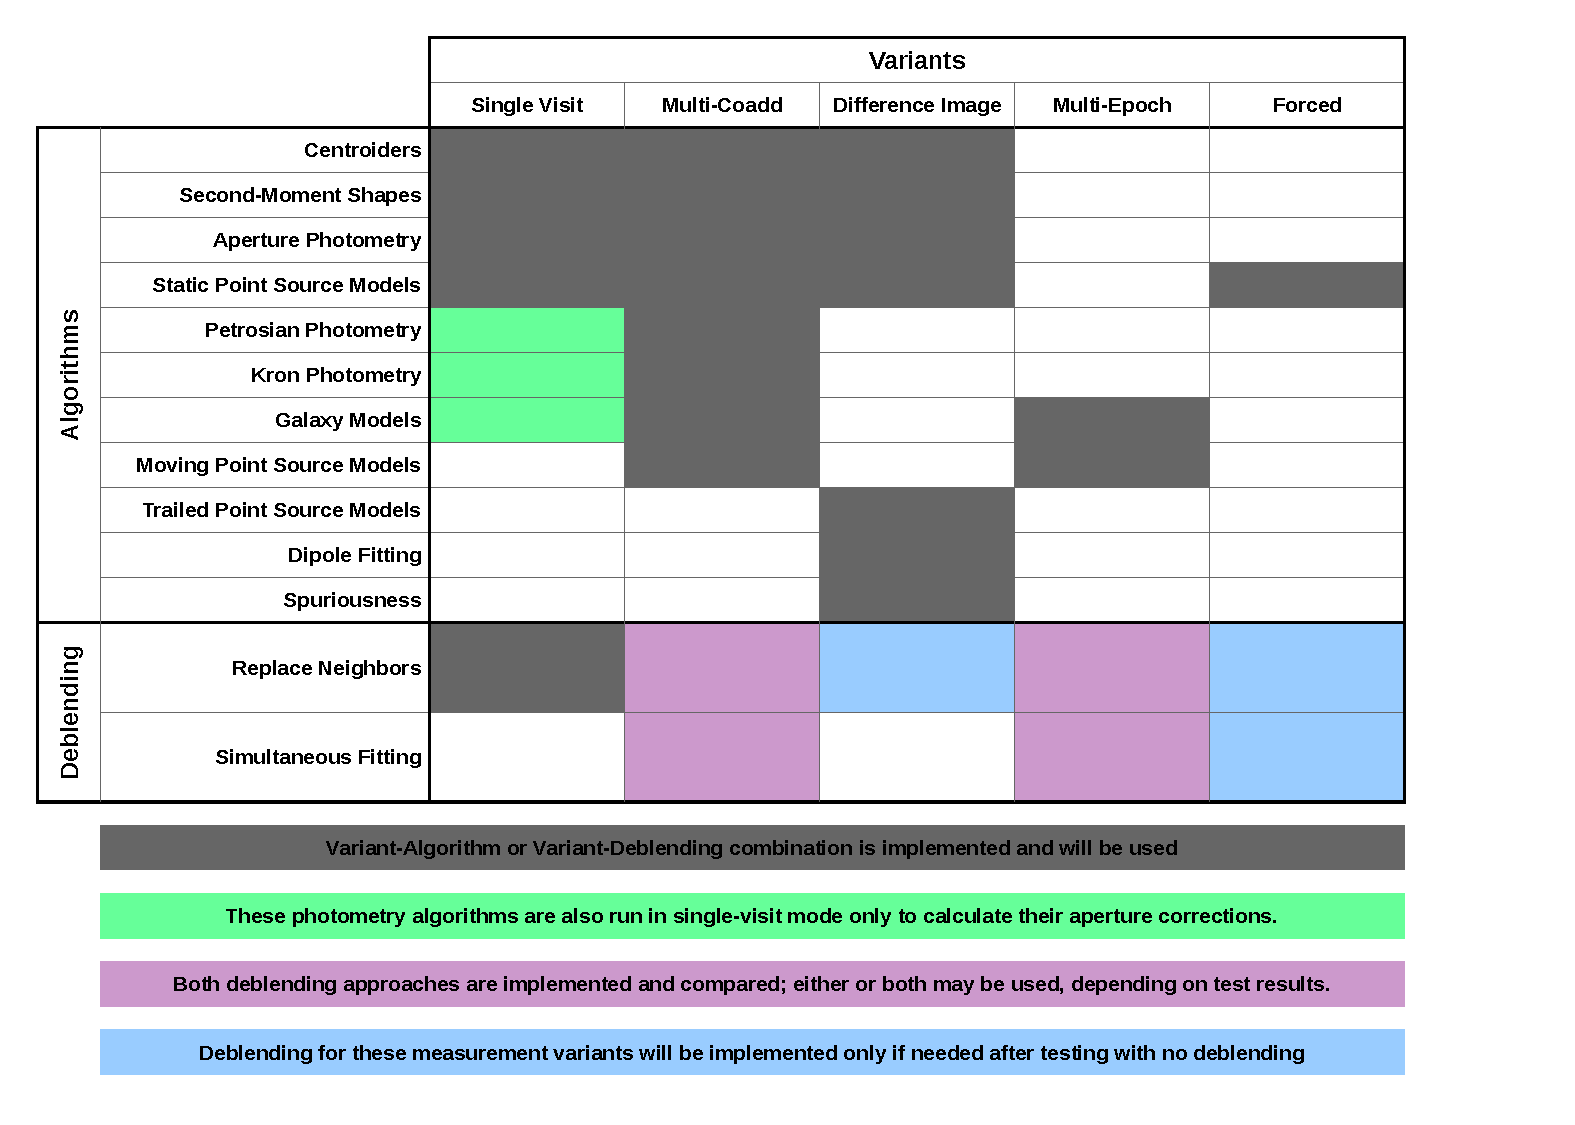
\includegraphics[width=\textwidth]{figures/measurement-matrix.pdf}
\caption{Matrix showing combinations of measurement variants, algorithms, and deblending approaches that will be implemented.
\label{fig:measurement-matrix}}
\end{figure}

\subsubsection{Variants}
Measurement is run in several contexts, but always consists of running an ordered list of algorithm plugins on either individual objects or families thereof.  Each context corresponds to different variant of the measurement driver code, and has a different set of plugin algorithms and approaches to measuring blended objects.

\paragraph{Single Frame Measurement:} Measure a direct single-visit CCD image, assuming deblend information already exists and can be used to replace neighbors with noise (see \ref{sec:acReplaceNeighborsWithNoise}).
\label{sec:acSingleFrameMeasurement}

Single Frame Measurement is run in both \hyperref[sec:apSingleFrameProcessing]{AP's Single Frame Processing pipeline}) and DRP's \hyperref[sec:drpBootstrapImChar]{BootstrapImChar}, \hyperref[sec:drpRefineImChar]{RefineImChar}, and \hyperref[sec:drpFinalImChar]{FinalImChar}.  It must be capable of running on wavefront sensor images, though this may require different plugin algorithms.

The driver for Single Frame Measurement is passed an input/output \hyperref[sec:spTablesSource]{SourceCatalog} and an \hyperref[sec:spImagesExposure]{Exposure} to measure.  Plugins take an input/output \hyperref[sec:spTablesSource]{SourceRecord} and an \hyperref[sec:spImagesExposure]{Exposure} containing only the object to be measured.

\paragraph{Multi-Coadd Measurement:} Simultaneously measure a suite of coadds representing different bandpasses, epoch ranges, and flavors.  This is run only in DRP's \hyperref[sec:drpMeasureCoadds]{MeasureCoadds} pipeline.
\label{sec:acMultiCoaddMeasurement}

The driver for Multi-Coadd Measurement is passed an input/output \hyperref[sec:spTablesObject]{ObjectCatalog} and a dict of \hyperref[sec:spImagesExposure]{Exposures} to be measured.  Plugins take an input/output \hyperref[sec:spTablesObject]{ObjectRecord} and a dict of \hyperref[sec:spImagesExposure]{Exposures}, each containing only the object to be measured.  Some plugins will also support simultanous measurement of multiple objects, which requires they be provided the subset of the \hyperref[sec:spTablesObject]{ObjectCatalog} to be measured and a dict of \hyperref[sec:spImagesExposure]{Exposures} containing just those objects.

\paragraph{Difference Image Measurement:} Measure a difference image, potentially using the associated direct image as well.  Difference image measurement is run in AP's \hyperref[sec:apAlertDetection]{Alert Detection} pipeline and DRP's \hyperref[sec:drpDiffIm]{DiffIm} pipeline.
\label{sec:acDiffImMeasurement}

The signatures of difference image measurement's drivers and algorithms are at least somewhat TBD; they will take at least a difference image \hyperref[sec:spImagesExposure]{Exposures} and a \hyperref[sec:spTablesSource]{SourceCatalog/SourceRecord}, but some plugins such as dipole measurement may require access to a direct image as well.  Because difference imaging dramatically reduces blending, difference image measurement may require any approach to blended measurement (though any use of the associated direct image would require deblending).

If preconvolution is used to construct difference images, but they are not subsequently decorrelated, the algorithms run in difference image measurement cannot be implemented in the same way as those run in other measurement variants, and algorithms that cannot be expressed as a PSF-convolved model fit (such as second-moment shapes and all aperture fluxes) either cannot be implemented or require local decorrelation.

\paragraph{Multi-Epoch Measurement:} Measure multiple direct images simultaneously by fitting the same \hyperref[sec:spWCS]{WCS}-transformed, \hyperref[sec:spPSF]{PSF}-convolved model to them.  Blended objects in Multi-Epoch Measurement will be handled by \emph{at least} fitting them simutaneously (\ref{sec:acSimultaneousFitting}), which may in turn require hybrid galaxy/star models (\ref{sec:acHybridModels}).  These models may then be used as templates for deblending and replace-with-noise (\ref{sec:acReplaceNeighborsWithNoise}) measurement if this improves the results.
\label{sec:acMultiEpochMeasurement}

Because the memory and I/O requirements for multi-epoch measurement of a single object or blend family are substantial, we will not provide a driver that accepts an \hyperref[sec:spTablesObject]{ObjectCatalog} and measures all objects within it; instead, the \hyperref{sec:drpMultiFit} pipeline will submit individual family-level jobs directly to the orchestration layer.  The multi-epoch measurement driver will thus just operate on one blend family at a time, and manage blending while executing its plugin algorithms.

Multi-epoch measurement for DRP only includes two plugin algorithms, so it is tempting to simply hard-code these into the driver itself, but this driver will also need to support new plugins in Level 3.

Multi-epoch measurement will also be responsible for actually performing forced photometry on direct images, which it can do by holding non-amplitude parameters for moving point-source models fixed and adding a new amplitude parameter for each observation.

\paragraph{Forced Measurement:} Measure photometry on an image using positions and shapes from an existing catalog.
\label{sec:acForcedMeasurement}

In the baseline plan, we assume that forced measurement will only be run on difference images; while forced photometry on direct images will also be performed in DRP, this will be done by multi-epoch measurement.

Because difference imaging reducing blending substantially, forced measurement may not require any special handling of blends.  If it does, simultaneous fitting (with point-source models) should be sufficient.

The driver for Forced Measurement is passed an input/output \hyperref[sec:spTablesSource]{SourceCatalog}, an additional input \hyperref[sec:spTablesReference]{ReferenceCatalog}, and an \hyperref[sec:spImagesExposure]{Exposure} to measure.  Plugins take an input/output \hyperref[sec:spTablesSource]{SourceRecord}, an input \hyperref[sec:spTablesReference]{ReferenceRecord} and an \hyperref[sec:spImagesExposure]{Exposure}.  If simultaneous fitting is needed to measure blends, plugins will instead receive subsets of the catalogs passed to the driver instead of individual records.

Forced measurement is used by the DRP \hyperref[sec:drpForcedPhotometry]{ForcedPhotometry} pipeline and numerous pipelines in AP.

\begin{note}[TODO]
Add references to specific AP pipelines that will use forced measurement.
\end{note}

\subsubsection{Algorithms}

\paragraph{Centroids}
\label{sec:acCentroidAlgorithms}
\begin{itemize}
\item should be equivalent to PSF model fit for stars
\item use larger weight function (TBD) for extended objects
\item need variant that doesn't require a PSF model (or can work with a poor guess) to run before PSF estimation.
\item need to have a version (possibly the main version) that works on wavefront sensors
\end{itemize}

\paragraph{Pixel Flag Aggregation}
\label{sec:acPixelFlags}
\begin{itemize}
\item Compute summary statistics of masked pixels in the neighborhood of the source/object.
\end{itemize}

\paragraph{Second-Moment Shapes}
\label{sec:acShapeAlgorithms}
\begin{itemize}
\item probably adaptive elliptical Gaussian weights, with fall back to unweightd, PSF-weighted, or some fixed Gaussian
\item add regularization for unresolved objects - avoid crazy ellipticities for objects much smaller than PSF
\item Should also compute moments of PSF model.
\item Need to have a version (possibly the main version) that works on wavefront sensors to characterize the donut-like out-of-focus sources.
\end{itemize}

\paragraph{Aperture Photometry}
\label{sec:acAperturePhotometry}

\begin{itemize}
\item Aperture fluxes are computed by summing the total flux within an elliptical region defined on the image.
\item Aperture fluxes are computed at a series of logarithmically spaced aperture sizes. Per the \DPDD{}, the total number of apertures will vary depending on the size of the source.
\item When computing fluxes for small apertures---for configurable values of ``small''--we use $\mathrm{sinc}$ interpolation \cite{Bickerton13}. For large apertures, we use a naive summation of pixel values.
\item May need to change ellipticity as a function of aperture radius.
\item If run before PSF estimation, will need a variant that does not rely on the PSF model to choose aperture size/ellipticity.
\end{itemize}

\paragraph{Static Point Source Models}
\label{sec:acStaticPointSourceModels}
\begin{itemize}
\item Fit PSF model for flux only (hold center fixed at centroid or reference value)
\item Doesn't use per-pixel variances for flux measurement, but might also provide measurement with per-pixel variances (for diagnostics?)
\end{itemize}

\paragraph{Kron Photometry}
\label{sec:acKronPhotometry}
\begin{itemize}
\item Compute Kron radius (hard to make this robust)
\item Compute flux in elliptical aperture at Kron radius.
\end{itemize}

\paragraph{Petrosian Photometry}
\label{sec:acPetrosianPhotometry}
\begin{itemize}
\item Compute Petrosian radius.  Harder than it seems due to need for improvements to splines? (ask RHL)
\item Compute flux in elliptical aperture at Petrosian radius.
\end{itemize}

\paragraph{Galaxy Models}
\label{sec:acGalaxyModels}
\begin{itemize}
\item Some sort of bulge+disk model.  Lots of need for experimentation.
\item Will Monte Carlo sample in MultiFit (and maybe on coadds, too, if that helps).
\item May also fit to PSF-matched coadds for consistent colors.
\item Will need to support simultaneous fitting (and sampling).
\item Hybrid model candidate
\end{itemize}

\paragraph{Moving Point Source Models}
\label{sec:acMovingPointSourceModels}
\begin{itemize}
\item Fit point source with flux, centroid, parallax, and proper motion parameters.
\item May need to support simultaneous fitting.
\item Might want to sample this too, at least if we fit it simultaneously with sampled galaxy models.
\item Hybrid model candidate
\end{itemize}

\paragraph{Trailed Point Source Models}
\label{sec:acTrailedPointSourceModels}
\begin{itemize}
\item Fit PSF convolved with line segment to individual images
\end{itemize}

\paragraph{Dipole Models}
\label{sec:acDipoleModels}
\begin{itemize}
\item Fit PSF dipole for separation and flux to a combination of difference image and direct image.
\item Deblending on direct image very problematic.
\end{itemize}

Arising primarily due to slight astrometric alignment or PSF matching errors between the two images, or effects such as differential chromatic aberration, flux “dipoles” are a common artifact often observed in image differences. These dipoles will lead to false detections of transients unless correctly identified and eliminated. Importantly, dipoles will also be observed in image differences in which a source as moved less than the width of the PSF. Such objects must be correctly identified and measured as dipoles in order to obtain accurate fluxes and positions of these objects. 

Putative dipoles in image differences are identified as a positive and negative source whose footprints overlap by at least one pixel. These overlapping footprints are merged, and only the sources containing one and only one positive and negative merged footprint are passed to the dipole modeling task. There is a documented degeneracy (\url{http://dmtn-007.lsst.io}) between dipole separation and flux, such that dipoles with closely-separated lobes of high flux are statistically indistinguishable from ones with low flux and wider separations. We remove this degeneracy by using the {\em pre-subtracted images} (i.e., the warped, PSF-matched template image and the pre-convolved science image) to constrain the lobe positions (specifically, to constrain the centroid of the positive lobe in the science image and of the negative lobe in the template image). This is done by first fitting and subtracting a second-order 2-D polynomial to the background within a subimage surrounding each lobe footprint in the pre-subtracted images to remove any flux from background galaxies (we assume that this gradient, if it exists, is identical in both pre-subtracted images). Then, a dipole model is fit simultaneously to the background-subtracted pre-subtracted images and the image difference. 

The dipole model consists of positive and negative instances of the PSF in the difference image at the dipole's location. The six dipole model parameters (positive and negative lobe centroids and fluxes) are estimated using non-linear weighted least-squares minimization (we currently use the Levenberg-Marquardt minimization algorithm). The resulting reduced $\chi^2$ and signal-to-noise estimates provide a measure by which the source(s) may be classified as a dipole. 

We have tested the described dipole measurement algorithm on simulated dipoles with a variety of fluxes, separations, background gradients, and signal-to-noise. Including the pre-subtracted image data clearly improves the accuracy of the measured fluxes and centroids. We have yet to thoroughly assess the dipole measurement algorithm performance on crowded stellar fields. Such crowded fields may confuse the parameter estimates (both centroids and/or fluxes) when using the pre-subtracted images to constrain the fitting procedure, and in such situations, we may have to adjust the prior constraint which they impose. 

\paragraph{Spuriousness}
\label{sec:acSpuriousnessAlgorithms}
\begin{itemize}
\item Some per-source measure of likelhood the detection is junk (in a difference image).
\item May use machine learning on other measurements or pixels.
\item May be augmented by spuriouness measures that aren't purely per-source.
\end{itemize}

\subsubsection{Blended Measurement}
\label{sec:acBlendedMeasurement}
\begin{itemize}
\item Integrate text from blended-measurement doc here.
\end{itemize}

\paragraph{Deblend Template Projection}
\label{sec:acDeblendTemplateProjection}
\paragraph{Neighbor Noise Replacement}
\label{sec:acReplaceNeighborsWithNoise}
\paragraph{Simultaneous Fitting}
\label{sec:acSimultaneousFitting}
\paragraph{Hybrid Models}
\label{sec:acHybridModels}

\label{Spatial Models}
\label{sec:acSpatialModels}
In many areas we will need to represent spatial models.  This will include models fit to sparse and non-uniformly sampled data.  We will support fitting Chebyshev polynomials and splines.  We will also support regression techniques like Gaussian Processes.

\subsection{Background Estimation}
\label{sec:acBackgroundEstimation}

Background estimation will be done on the largest scale feasible first.  In the case of Alert Production, this may be on the size of a chip.  In DRP, we expect this to be on a full focalplane.  An initial low order estimate will be made on a large scale.  Each chip will be divided into subregions.  For each subregion, the median of the non-masked pixels will be computed.  All values for all chips will be fit by an appropriate function (see \S \ref{sec:acSpatialModels}).  This will provide a low order background estimation in focal plance coordinates.  Note that this can only be done if the instrument signature removal is very high fidelity.  Any sharp discontinuity could cause problems with fitting a smooth function.

A higher order background model can be computed per chip.  First, the low order background is subtracted from the image.  The non-masked pixels will again be binned on a finer grid avoiding bright objects.  The median in each bin is fit by an appropriate function.  In practice, this process will likely be iterative.

In the case of Alert Production, there will be no full focalplane model since we expect to process only a single chip in each thread.  In this case, we constrain the background with the available un-masked pixels without removing a global background first.  Note that image differencing is still possible even in the scenario where there are no unmasked pixels in the science image.  The background can be modeled as a part of the PSF matching process.  We will want to do background modeling and subtraction in Alert Production when possible because we will want to do calibrated photometry.  Even though these measurements are not persisted for science us, they will be very useful for debugging and QA.

If there are so few un-masked pixels in the entire focalplane that even a low order global background is impossible to model, we will not compute a background model.  Instead, we will do crowded field photometry only \ref{????}

\begin{note}[Crowded fields and composition]
Requirements included working in crowded fields.  I think estimating a full focalplane model is the best we can do.  If there are no unmasked pixels in the entire FoV, I don't think there is much we can do.
I didn't explicitly talk about composition of background models, but this takes that into account by allowing a global model to be subtracted from the single chip image before a higher order model is fit.
\end{note}

\subsection{Build Background Reference}
\label{sec:acBuildBackgroundReference}
AUTHOR: Simon
\begin{itemize}
\item Given multiple overlapping visit images (already warped to a common coordinate system), synthesize a continuous single-epoch image that can be used as a reference for background matching.
\end{itemize}

\subsection{PSF Estimation}
\label{sec:acPSFEstimation}

\subsubsection{Single CCD PSF Estimation}
\label{sec:acSingleCCDPSF}

Single CCD PSF estimation needs to be run in both Alert Production and in in Data Release Processing.  In Alert Production it will be the final PSF model for both direct and difference image measurement.  In Data Release Processing, it will be used as an initial bootstrapping step to start off image characterization.  We do not intend to include chromatic effects in the PSF at the single CCD estimation phase.

The first step is to select a set of suitable stars to use as PSF exemplars.  This can be done by finding clusters in second moment space.  In production, we expect that an external catalog with PSF candidates that have been show to be non-varying and isolated will produce better results.

Once a set of candidate stars is selected each star is fit by a set of appropriate basis functions: e.g. shapelets.  The PSF is approximated by
\[
P = \Sigma_n c_n\Psi_n
\]
where $\Psi_n$ is the $n^{th}$ basis function, and $c_n$ is the coefficient for that basis function.  We can solve for the coefficients in the least squares sense using a QR decomposition or similar technique.  We then have an estimate of the PSF at several locations on the chip.  For each of the coefficients we can fit 2D Chebyshev polynomials to each coefficient to model the spatial variation in each component (see \ref{sec:acSpatialModels}).  By interpolating the fit coefficients, we can derive an estimate of the PSF at any point in the chip.

The order of the spatial model cannot excede number of PSF exemplars in the frame.  If there is only a single PSF candidate star, we will assume the PSF is constant across the CCD.  In the case of no PSF candidate stars, we will assume a double Gaussian PSF with width set by observation metadata: e.g. FWHM from the guiding system.

\begin{note}[Do we need something more complex?]
We can get arbitrarily complex, but I don't thinkn we need a more complex system in the baseline until we show this won't work.
\end{note}

\subsection{Wavefront Sensor PSF Estimation}
\label{sec:acWavefrontSensorPSF}
AUTHOR: Jim
\begin{itemize}
\item Build an approximate PSF model using only the very brightest stars in the wavefront sensors.  Because WF sensors are out-of-focus, these stars may be saturated on science CCDs.
\item Model can have very few degrees of freedom (very simple optical model + elliptical Moffat/Double-Gaussian?)
\item Only needs to be good enough to bootstrap PSF model well enough to bootstrap processing of science images (but it needs to work in crowded fields, too).
\item Being able to go to brighter magnitudes may be important in crowded fields because the shape of the luminosity function may make it easier to find stars with (relatively) significant neighbors.
\end{itemize}

\subsubsection{Full Visit PSF Estimation}
\label{sec:acFullVisitPSF}
AUTHOR: Jim
\begin{itemize}
\item Decompose PSF into optical + atmosphere.
\item May also use wavefront sensors.
\item Constrain model with stars, telemetry, and wavefront data.
\item Wavelength-dependent.
\item Used in RefineImChar in DRP.
\item Must include some approach to dealing with wings of bright stars.
\end{itemize}

\subsection{Model Spatial Variation of PSF}
\subsubsection{Within a CCD}
\label{sec:acModelSpatialPSF}

\begin{itemize}
\item Estimate PSF at discrete locations using a set of basis functions
\item Fit interpolation functions to fit coefficients to enable interpolation
\end{itemize}
\subsubsection{Over a focal plane -- Do we need this?}

\subsection{Aperture Correction}
\label{sec:acApCorr}
AUTHOR: Jim
\begin{itemize}
\item Measure curves of growth from bright stars (visit-level, at least in DRP)
\item Correct various flux measurements to infinite (CCD-level)
\item Propagate uncertainty in aperture correction to corrected fluxes; covariance is tricky.
\end{itemize}

\subsection{Astrometric Fitting}
\label{sec:acAstrometricFitting}
AUTHOR: Simon
\subsubsection{Single CCD}
\label{sec:acSingleCCDAstrometricFit}
Used by AP, probably (RHL worries we might need full-visit)

AP will need to do reasonably good astrometeric calibration on single frames in order to do the relative warping between the template and science images.  We will use the internal reference catalog used in DRP as the reference catalog.  This will be based on astrometry from an external source and will be extended using high quality measurements on coadds from DRP.

We will use a matching algorithm like that outlined in \cite{tabur04}.  Once we match, a 2D polynomial solution will be fit to minimize the residual.

\begin{note}[Dependency]
This introduces a dependency on DRP's internal reference catalog not capture elsewhere.
\end{note}

\subsubsection{Single Visit}
\label{sec:acSingleVisitAstrometricFit}
Full visit astrometric fitting will be done as a bootstrapping step toward higher quality calibration in DRP.  All measurements in the visit will be projected to a tangent plane, taking into account all knowledge of the sensor arrangement and optics.  The reference catalog (likely the DRP reference catalog) will be projected to the same tangent plane.

Sources will be matched, again using a \cite{tabor04} like algorithm.  Once the reference and observations are matched, a multi-component WCS will be fit.  We expect the components will be related to residuals on the optical model and will included a component to account for the Von Karman turbulence.

\subsubsection{Joint Multi-Visit}
\label{sec:acJointAstrometicFit}
In the case where there are multiple visits overlapping the same part of the sky, e.g. a patch, we can leverage multiple realizations to beat down the random contribution of the atmosphere to get a better estimate of the optical model and the atmospheric contribution per visit.

The catalogs are stacked and matched using a multi-matching algorithm like OPTICS.  At this point, the measurements can be matched to an external catalog for the purposes of absolute astrometry.  With all measurementss in hand, a multi-component WCS is fit to all measurements at the same time on order to minimize the residual from the mean position for each object.

\subsection{Photometric Fitting}
\label{sec:acPhotometricFitting}
\subsubsection{Single CCD (for AP)}
\label{sec:acSingleCCDPhotometricFit}
\begin{itemize}
\item Match to photometric calibration reference catalog
\item Calculate single zeropoint using available color terms
\end{itemize}
\subsubsection{Single Visit}
\label{sec:acSingleVisitPhotometricFit}
\begin{itemize}
\item Fit zeropoint (and some small spatial variation?) to all CCDs simultaneously after matching to reference catalog.
\item Need for chromatic dependence unclear; probably driven by AP.
\end{itemize}

what is this zeropoint going to be used for?  I don't see how this will add much over just the single CCD fitted zeropoints.

I think PanStarrs had a lot of success imaging a standard field every night and then just fitting a nightly zeropoint.  Twilight might be a good time to observe a standard field in all the filters that are expected to be used in the night.  Then you can have a rough zeropoint for the night and only update if conditions change?


\subsubsection{Joint Multi-Visit}
\label{sec:acJointPhotometricFit}
\begin{itemize}
\item Derive SEDs for calibration stars from colors and reference catalog classifications.
\item Utilize additional information from wavelenth dependent photometric calibration built by calibration products production.
\item Fit zeropoint and possibly perturbations to all CCDs on multiple visits simultaneously after matching to reference catalog.
\end{itemize}

My understanding for the ubercal:
\begin{itemize}
\item{you have a list of observed magnitudes that are post ISR, but pre zeropoint corrected}
\item{You can assign a rough SED to each star based on its color.}
\item{Use the atmospheric transmission information + SED of star to correct the magnitude to a fiducial filter bandpass}
\end{itemize}

Because the number of stars gets ridiculously large, I solved distinct overlapping regions of sky in parallel.  I think I used a single CCD as the patch size.  Once all the regions converge, you can run the same ubercal matrix solution to tie the patches together.  So, in equations, the fist step is to solve:
\begin{equation}
m_{ij} = m_i + z_j
\end{equation}
where $m_{ij}$ is an observed magnitude of star with true magnitude $m_i$ on observation $j$.  While it is possible to include more terms (say, fit out flat-fielding errors at the same time), that makes it much harder to solve in parallel, it's easy to make the problem degenerate, and it can slow things down rapidly. 

This method leaves a "floating zeropoint" in the solution (if you ad X to all the $m_i$'s, and -X to all the $z_j$'s the solution is the same).  If one solves regions of the sky independently, then the floating zeropoints of each region (say a HEALpixel) need to be matched:
\begin{equation}
p_{ij} = p_i + HP_j
\end{equation}
One thing that is still lacking is that it's not clear what uncertainties to put in for the different $p_{ij}$'s (unlike the observed magnitudes where it's relatively easy to calculate a reasonable uncertainty).  We also don't naturally get uncertainties out of the solvers, so that's something that needs to be worked on.

So, after solving for all the magnitudes, and merging all the patch zeropoints, there's still the final floating zeropoint (in each filter) that needs to be removed.  People like using WD for this type of thing since they have spectra that should be theoretically calculated to millimag precision.  There's also speculation that GAIA could provide a good way to do the flux calibration.  

It occurs to me that the ubercal problem can be pretty well described with a latex drawing and writing out the matrix that goes with it.  I can work on that if you want.



\subsection{Retrieve Diffim Template for a Visit}
\label{sec:acRetrieveTemplate}
In difference imaging a major contributor to the quality of the difference image is the choice of template.  We expect that the DRP template generation algorithm will be quite complex.  It will potentially involve synthesizing multiple monochromatic templates that will be used to model the effects of DCR.

Ideally, the retrieval will be to select the correct bounding box from the correct master template for the current observation.  If not, we expect the template generation algorithm will provide an algorithm to interpret the templates.

\subsection{PSF Matching}
\label{sec:acPSFMatching}

The essence of image subtraction is to astrometrically register the science image $S(x,y)$ and template image $T(x,y)$, and then match their point spread functions (PSFs) of so that they may be subtracted pixel by pixel. The PSFs are the time--averaged transfer functions of a point source through the Earth's atmosphere, telescope optics, and into the silicon of the detector before being read out. We assume that the science image can be modeled as a convolution of the template image by a PSF--matching kernel $\kappa(u,v;x,y)$, i.e., $S = \kappa \otimes T$. (Indices $u,v$ indicate that the kernel itself is a 2--dimensional function, which varies as a function of position $x,y$ in the image; during convolution and correlation there is an implicit summation over $u,v$.) Then the difference image, upon which new or variable sources are detected, is given by $D = S - (\kappa \otimes T)$. 

\subsubsection{Image Subtraction}
\label{sec:acImageSubtraction}
\begin{itemize}
\item Match template image to science image, as in Alert Production and DRP Difference Image processing.
\item Includes identifying sources to use to determine matching kernel, fitting the kernel, and convolving by it.
\end{itemize}

The current implementation of the PSF matching algorithm is summarized in detail by Becker, et al. (2013) (\url{http://ls.st/x9f}).  We model the PSF--matching kernel by decomposing it into a set of basis functions $\kappa(u,v) = \sum_i a_i \kappa_i(u,v)$ \citep{Alard98}, where the coefficients are determined via ordinary least-squares estimation:
%
\begin{eqnarray}
C_i & \equiv & (\kappa_i \otimes T); \\ \nonumber
b_{i}  & = & \sum_{x,y} {{C_i(x,y) S(x,y)}\over{\sigma^2(x,y)}};   \nonumber \\ 
M_{ij} & = & \sum_{x,y} {{C_i(x,y) C_j(x,y)}\over{\sigma^2(x,y)}};  \nonumber \\ 
a_{i}  & = & M^{-1}_{ij} b_{j}. \nonumber 
\label{eq-soln}
\end{eqnarray}
%
\noindent
$\sigma^2(x,y)$ is the per--pixel variance stored in the {\tt   variance} plane of each LSST {\tt exposure}. To generate a spatially varying model for the kernel, we further decompose the relative weights of the basis coefficients $a_i$ into spatially-varying low-order polynomials, i.e. $\kappa(u,v;x,y) = \sum_i a_i(x,y) \kappa_i(u,v)$. We also allow for a spatially-varying differential background between the two images $b(x,y)$ that may be fit for using a low--order polynomial \citep{Alard98,Alard00}. The image difference is then $D(x,y) = S(x,y) - T(x,y) \otimes \kappa(u,v;x,y) - b(x,y)$. 

The basis functions $\kappa_i(u,v)$ are a degree of freedom in this problem. Following \citep{Alard98}, we use a set of $\rm nGauss = 3$ Gaussians, each with a different width $\sigma_i$, and each modified by a Laguerre polynomial to a given order (see below). Following more recent studies studies \citep[e.g.][]{Israel07}, we parameterize these different Gaussian widths via a single ratio $\beta$, such that $\sigma_{i+1} = \beta \times \sigma_{i}$ with $\beta = 2.0$. (We note that all constants are defined by {\tt Config} variables and may be adjusted on a per-use basis). We set the overall scale for the $\sigma$ by noting that, under the assumption that the PSFs of the images are Gaussian ($\sigma_S$ for the science image and $\sigma_T$ for the template image), the $\sigma_{\kappa}$ of the matching kernel should be simply $\sigma_{\kappa}^2 = \sigma_S^2 - \sigma_T^2$. We use this canonical width for the central Gaussian in the basis sequences (i.e., $\sigma_{i=2} \equiv \sigma_{\kappa}$ when using three Gaussians bases). Each of the three default kernel basis functions are modified by Laguerre polynomials up to order $\rm degGauss = [4, 2,   2]$, respectively. This results in a total number of (non-spatially varying) bases of $\sum_i^{\rm nGauss} ({\rm degGauss}_i+1)\times({\rm   degGauss}_i+2)/2$, or 27 given the aforementioned defaults. 

A spatially-invariant matching kernel $\kappa(u,v)$ is determined separately for image substamps centered on multiple kernel candidates across the image. The kernel candidates are selected using the {\tt   DiaCatalogSourceSelector} to query the appropriate reference catalog for appropriate sources to use for PSF matching. This selector allows the user to specify the brightness and color range of the objects, toggle star or galaxy selection, and to include variable objects or not. Sources are vetted for signal-to-noise and masked pixels (in both the template and science image). The matching (spatially-invariant) kernel models $\kappa_j(u,v)$, determined for each kernel candidate $j$ as described above, are examined and filtered by various quality measures. The resulting ensemble of filtered kernel models is used to constrain the spatially-varying kernel model $\kappa(u,v;x,y)$ by fitting the spatially-varying basis kernel coefficients $a_i(x,y)$ with a $N^{th}$-order 2-dimensional Chebyshev polynomial. This results in the final full spatial solution $\kappa(u,v;x,y) = \sum_i a_i(x,y) \kappa_i(u,v)$, which may be evaluated at each location $(x,y)$ in the image for convolution. 

Detection on the difference image occurs through correlation of $D(x,y)$ with the science image's PSF, yielding optimally filtered detection image $D'(x,y) = D(x,y) \circ PSF_S(u,v;x,y)$ where $\circ$ denotes correlation (currently the DM stack uses convolution instead of correlation). The values of the pixels in $D'(x,y)$ provide a maximum likelihood estimate of there being a point source at that position. Detection occurs by simply finding pixels that are more than $N \times \sigma$ above the square root of the per--pixel variance. Alternatively, the science image may be {\em pre-convolved} with a kernel similar to its PSF, in which case the resulting difference image $D(x,y)$ is already filtered for detection. This latter option has the additional advantage that it help us avoid requiring {em deconvolution} of the template image, in cases when the template has a wider PSF than the science image. 

\subsubsection{PSF Homogenization for Coaddition}
\label{sec:acPSFHomogenization}
\begin{itemize}
\item Match science image to predetermined analytic PSF, as in PSF-matched coaddition.
\end{itemize}

In PSF-matched coaddition, input images are convolved by a kernel that matches their PSF to a predefined constant PSF before they are combined. This so-called ``model PSF matching'' uses the PSF-matching algorithm described in the previous section to match the PSF {\em   model} from an exposure to a pre-determined template (e.g., a constant-across-the-sky double Gaussian) PSF model. For this task, we realize each PSF model into an exposure-sized grid, and then utilize those as kernel candidates as input for the PSF matching algorithm described above. 

\subsection{Image Warping}
\label{sec:acWarping}
AUTHOR: Jim
\subsubsection{Oversampled Images}
\label{sec:acOversampledWarping}

Oversampled images are warped to a new \hyperref[sec:spWCS]{WCS} and resampled using a two dimensional Lancsoz kernel of configurable order. The baselined default order is 3.

The one dimensional Lancsoz kernel of order $a$ is defined as
\[
L(x) = \begin{cases}
       \operatorname{sinc}(x)\, \operatorname{sinc}(x/a) & \text{if}\;\; -a < x < a\\ 0 & \text{otherwise.}
       \end{cases}
\]
The two dimensional Lancsoz kernel is $L(x, y) = L(x) \cdot L(y)$.

For each integer pixel position in the remapped image, the associated pixel position in the source image is determined using the source and destination WCS. The warping kernel is then applied to the source image to compute the remapped pixel value. A flux conservation factor is applied based on the relative sizes of the pixel in the source and destination WCS.

For performance reasons, it is desirable to reduce the total number of WCS calculations. It is therefore acceptable to perform the mapping between source and destination images over a regular grid and linearly interpolate between grid points, rather than mapping every pixel independently.

Since chromaticity is accounted for in the \hyperref[sec:spPSF]{PSF} rather than the WCS, no special account is taken of color when warping.

\begin{note}
The above describes the current warping implementation in afw. We should identify deficiencies with the current implementation to establish resource requirements.
\end{note}

\subsubsection{Undersampled Images}
\label{sec:acUndersampledWarping}
\begin{itemize}
\item Can use PSF model as interpolant if we also want to convolve with PSF (as in likelihood coadds).  Otherwise impossible?
\end{itemize}
\subsubsection{Irregularly-Sampled Images}
\label{sec:acFixPixelAreaVariations}
\begin{itemize}
\item Approximate procedure for fixing small-scale distortions in pixel grid.
\end{itemize}

\subsection{Image Coaddition}
\label{sec:acCoaddition}
AUTHOR: Jim
\begin{itemize}
\item Must be able to do generalized outlier rejection, using histograms of detection masks produced on difference images.
\item Needs to propagate full uncertainty somehow.
\item Needs to propagate PSFs.
\item Needs to propagate wavelength-dependent photometric calibration.
\item May need to propagate larger-scale per-exposure masks to get right PSF model or other coadded quantities.
\item Should be capable of combining coadds from different bands and/or epoch ranges ranges as well as combining individual exposures.
\item Also needs to support combining snaps
\end{itemize}

\subsection{DCR-Corrected Template Generation}
\label{sec:acDCRTemplates}
%AUTHOR: Simon

Refraction by the Earth's atmosphere results in a dispersion of an
astronomical image along the ``parallactic angle''. This amplitude of
this dispersion depends on the spectral energy distribution (SED) of
the source and the refractive index of the atmosphere. Differential
chromatic refraction (DCR) refers to the SED dependent refraction
within a given photometric passband. For the airmass range of the LSST
and its filter complement the amplitude of the DCR could be up to 1.1
arcsec in the u band and 0.8 arcsec in the g band. Image subtraction
templates that do not account for DCR will result in dipoles in the
subtracted images.

The baseline approach for minimizing DCR induced dipoles in image
differences is to selected coadded templates that are close in airmass
\autoref[sec:templateSelect]. This will identify three airmass bins (XXX
where is this defined) from which PSF matched coadds will be generated
(ref).

Given the sensitivity of the number of false positives to the
astrometric accuracy of the registration of images and the dependence
of this astrometric accuracy on DCR we plan to define an interpolation
scheme for generating DCR corrected templates.

\subsubsection{Refraction from the atmosphere }
%reference stone and community posting on DCR

Refraction is dependent on the local index of refraction of air $n_0(\lambda)$ at the observatory:
\begin{align}
	n_0(\lambda) =&1 + \left(\left[2371.34 +\frac{683939.7}{130 - \sigma(\lambda)} +\frac{4547.3}{38.9 - \sigma(\lambda)^2}\right] D_s 
		+ \left(6487.31 + 58.058 \sigma(\lambda)^2 - 0.71150 \sigma(\lambda)^4 +0.08851 \sigma(\lambda)^6\right) D_w \right)\times 10^{-8} \label{eqn:index_refraction}\\*
	& where \nonumber\\*
	\sigma(\lambda) &= 10^4 /\lambda \;\;\;\;\left(\mu m^{-1}\right)\nonumber \\*
	D_s =& \left[1 + (P_s-P_w) \left(57.90\times10^{-8} - \frac{9.3250\times10^{-4}}{T}+\frac{0.25844}{T^2}\right)\right] \frac{(P_s-P_w)}{T} \nonumber \\*
	D_w =& \left[1 + P_w \left(1 + 3.7\times10^{-4} P_w\right)\left(-2.37321\times10^{-3} + \frac{2.23366}{T} - \frac{710.792}{T^2} + \frac{7.75141\times10^4}{T^3}\right)\right] \frac{P_w}{T} \nonumber \\
	P_w =& RH\times 10^{-4} \times e^{(77.3450 + 0.0057 T - 7235.0/T)}/T^{8.2} \nonumber
\end{align}
where the parameters $D_s$ and $D_w$ are the density factors for dry air and water vapor, respectively, taken from \cite{Owens:67}.


The ratio of local gravity at the observing site to $g = 9.81 m/s^2$ is given by
\begin{equation}
\kappa = g_0/g = 1 + 5.302\times 10^{-3} \sin^2\phi - 5.83\times 10^{-6} \sin^2(2\phi) - 3.15\times 10^{-7} h \label{eqn:kappa}
\end{equation}

and, assuming an exponential density profile for the atmosphere, then
the ratio $\beta$ of the scale height of the atmosphere to radius of
the observing site from the Earth's core can be approximated by
\begin{equation}
	\beta =  4.5908\times 10^{-6} T \label{eqn:beta}
\end{equation}
where $m$ is the average mass of molecules in the atmosphere, $R_\oplus$ is the radius of the Earth, $k_B$ is the Boltzmann constant, and $g_0$ is the acceleration due to gravity at the Earth's surface.


Refraction, as a function of wavelength is then given by, 
\begin{align}
R(\lambda) &= r_0 n_0(\lambda) \sin z_0 \int_1^{n_0(\lambda)} \frac{dn}{n \left(r^2n^2 -r_0^2n_0(\lambda)^2\sin^2z_0\right)^{1/2}} \nonumber\\
&\simeq \kappa (n_0(\lambda) - 1) (1 - \beta) \tan z_0 - \kappa (1 - n_0(\lambda)) \left(\beta - \frac{n_0(\lambda) - 1}{2}\right) \tan^3z_0
\end{align}

\begin{table}[h!]
	\begin{center}
	\begin{tabular}{c | c | c | c}
		Parameter & valid range & description & units \\
		\hline
		$P_s$& $0$ mbar$ < P_s < 4000$ mbar & Atmospheric pressure & millibar  \\
		$RH$ & $0\% < RH < 100\%$ & Relative humidity & Percent \\
		$\lambda$& $2302$\AA{}$ < \lambda < 20,586 $\AA{} & Wavelength  & Angstroms \\
		$T$& $250K < T < 320K$ & Temperature & Kelvin \\
		$\phi$ & $0^\circ \leq \phi < 360^\circ$ & Latitude of the observing site & Degrees \\
		$h$ & $0\,m\leq h$ & Elevation of the observing site & meters \\
		$z_0$ & $0^\circ\leq z_0 < 75^\circ$ & Zenith angle & Degrees
		
	\end{tabular}
	\end{center}
	\caption{Definition of parameters and their units}
	\label{table:parameters}
\end{table}
%\vspace{-0.7cm}

\subsubsection{Generating a DCR corrected template}

Given a set of observed images, $O(x, z)$, at an airmass of $z$, and
assuming that we know the wavelength dependence of the refraction, we
can model the corresponding image at the zenith (or any other
airmass), $I(x, 0)$. For simplicity, we will consider only a single
row of a sensor as comprising an image, that the direction of the DCR
is aligned along, and we will assume the PSF is constant between
images. 

The impact of DCR is to move flux between pixels as a function of
airmass and wavelength. This shift, $R(\lambda, z)$ can be treated as
a a shift operator or a convolution, $D(\lambda, z)$ and is known
given the refractive index of the atmosphere.  If we consider that the
zenith image can be decomposed into a linear sum over wavelength, i.e.,
\begin{equation}
I(x', 0) = \sum_\lambda I(x', 0, \lambda) 
\end{equation}
then the observed set of images are given by,
\begin{equation}
O(x, z) = \sum_\lambda I(x',\lambda) \otimes D(\lambda, z) 
\label{eq:convDCR}
\end{equation}

Solving for $I(x,\lambda)$ is then a regression problem that can be 
solve for by minimizing
\begin{equation}
\chi^2 = \sum_x O(x) - \sum_\lambda I(x',\lambda) \otimes D(\lambda) 
\end{equation}

There are a number of possible approaches for finding the ``zenith''
image.  The convolution can be written as a transfer matrix, $T$,
where the elements of the matrix correspond to the pixel values of
$ I(x',\lambda)$ that map to the pixel values of $O(x, z)$ given the
refraction. Under this mapping, we can write the linear equations as
$TI=O$ and by inverting the matrix solve for $I$. While,  $T$, is
clearly sparse the number of terms that must be solved for given the
number of wavelengths $\lambda$ that $I$ is decomposed into means that
we require a heavily regularized regression.

The initial implementation for the DCR corrected template will invert
the linear equations assuming smoothness in the between adjacent
pixels and as a function of wavelength by adopting first and second
order finite difference matrices (ref nate).  

2 separate regularizations smooth in pixel and smooth in wavelength

matrix extends in size.

An prototype
implementation has been demonstrated for the 1D case.  A second
approach will be to forward model the problem by iteratively updating
$I$ based on the set of observations (ref, budavari). 

For each approach the number of wavelength bins that $I(x)$ can be
decomposed into will depend on the number of observations at different
airmass. The assumption of a constant PSF will clearly not hold for
the LSST observations but can be incorporated within the convolution
\autoref{eq:convDCR} or addressed through a separable, wavelength
dependent, PSF convolution. The robustness of these techniques will
need to be evaluated for low signal-to-noise sources and in the
presence of scattered light and artifacts. 


\subsection{Image Decorrelation}
\label{sec:acImageDecorrelation}
\subsubsection{Difference Image Decorrelation}
\label{sec:acDiffImDecorrelation}

In situations where the signal-to-noise in the template image is not insignificant (e.g., when the template is constructed by co-addition of a small number of exposures), the resulting image difference will contain autocorrelated noise arising from the convolution of the template with the PSF matching kernel prior to subtraction. This will result in innaccurate estimates of thresholds for {\tt diaSource} detection if the (potentially spatially-varying) covariances in the image difference are not properly accounted for.

A viable alternative in the case of noisy template images is to construct a difference image with a flat noise spectrum, like the original input images \citep{Kaiser04, Zackay16}. This simply involves multiplying the image difference by a term which removes its frequency dependence,

\begin{equation}
  D(k) = \left[S(k) - \kappa(k) T(k)\right]\sqrt{\frac{\sigma_S^2+\sigma_T^2}{\sigma_S^2 + \kappa^2(k)\sigma_T^2}},
  \label{eqn:decorr}
\end{equation}

\noindent
where $S$ is the science image, $T$ is the template, $\sigma_S^2$ and $\sigma_T^2$ are their respective variances, and $\kappa$ is the PSF-matching kernel which, when convolved with the template, matches the PSF of the template to that of the science image. $\kappa$ may be solved for (in real space) as described in Section~\ref{sec:acPSFMatching}. Then the multiplication by the square-root term in Equation~\ref{eqn:decorr} may be interpreted as applying a post-image-differencing convolution kernel which ``removes'' the pixel-wise correlation which was added by convolution of the template by the PSF-matching kernel. The PSF of the resulting decorrelated difference image $\phi_D$ then equals the PSF of the science image $\phi_S$, convolved with the post-differencing kernel:

\begin{equation}
  \phi_D(k) = \phi_S(k) \sqrt{\frac{\sigma_S^2+\sigma_T^2}{\sigma_S^2 + \kappa^2(k)\sigma_T^2}}.
\end{equation}

We are investigating this approach and have shown that, for idealized situations, the resulting image differences are statistically indistinguishable from those generated using the ``Proper image subtraction'' technique proposed by \cite{Zackay16}.

Issues arising from complications often seen in real-world data such as spatially-varying PSFs and/or poorly-evaluated matching kernels, spatially variable backgrounds and/or noise, and possibly non-Gaussian or heteroschedastic noise need to be further evaluated. Such tests are currently underway on simulated and real data. These tests could highlight the advantages of the method proposed here over the proposal of \cite{Zackay16}, including: no requirement for accurate measurement of the PSFs of the science or template images, and thus the ability to to account for errors in astrometric alignment and to directly model spatially varying differential PSFs.

\subsubsection{Coadd Decorrelation}
\label{sec:acCoaddDecorrelation}
AUTHOR: Jim
\begin{itemize}
\item Fourier-space/iterative deconvolution of likelihood coadds, as in DMTN-15.
\item Need to test with small-scale research before committing to this approach.
\end{itemize}

\subsection{Star/Galaxy Classification}
\label{sec:acClassification}
AUTHOR: Jim
\subsubsection{Single Frame S/G}
\label{sec:acSingleFrameClassification}
\begin{itemize}
\item Extendedness or trace radius difference that classifies sources based on single frame measurements that can utilize the PSF model.  Used to select single-frame calibration stars, and probably aperture correction stars.
\end{itemize}
\subsubsection{Multi-Source S/G}
\label{sec:acJointCalClassification}
\begin{itemize}
\item Aggregate of single-visit S/G post-PSF numbers in jointcal.
\end{itemize}
\subsubsection{Object Classification}
\label{sec:acObjectClassification}
\begin{itemize}
\item Best classification derived from multifit and possibly variability.
\end{itemize}

\subsection{Variability Characterization}
\label{sec:acVariabilityCharacterization}

Following the \DPDD{}, lightcurve variability is characterized by providing a series of numeric summary `features' derived from the lightcurve. The DPDD baselines an approach based on Richards et al. \cite{Richards11}, with the caveat that ongoing work in time domain astronomy may change the definition, but not the number or type, of features being provided.

Richards et al. define two classes of features: those designed to characterize variability which is periodic, and those for which the period, if any, is not important. We address both below.

All of these metrics are calculated for both Objects (\DPDD{} table 4, \texttt{lcPeriodic} and \texttt{lcNonPeriodic}) and DIAObjects (\DPDD{} table 2, \texttt{lcPeriodic} and \texttt{lcNonPeriodic}). They are calculated and recorded separately in each band. Calculations for Objects are performed based on forced point source model fits (\DPDD{} table 5, \texttt{psFlux}).  Calculations for DIAObjects are performed based on point source model fits to DIASources (\DPDD{} table 1, \texttt{psFlux}). In each case, calculation requires the fluxes and errors for all of the sources in the lightcurve to be available in memory simultaneously.

\subsubsection{Characterization of periodic variability}

\begin{itemize}

\item{Characterize lightcurve as the sum of a linear term plus sinusoids at three fundamental frequencies plus four harmonics:
\begin{align}
y(t) &= ct + \sum_{i=1}^{3} \sum_{j=1}^{4} y_i(t|j f_i) \\
y_i(t|j f_i) &= a_{i,j} \sin(2 \pi j f_i t) + b_{i, j} \cos(2 \pi j f_i t) + b_{i, j, 0}
\end{align}
where $i$ sums over fundamentals and $j$ over harmonics.
}
\item{Use iterative application of the generalized Lomb-Scargle periodogram, as described in \cite{Richards11}, to establish the fundamental frequencies, $f_1$, $f_2$, $f_3$:
\begin{itemize}
  \item{Search a configurable (minimum, maximum, step) linear frequency grid with the periodogram, applying a $\log f/f_N$ penalty for frequencies above $f_N = 0.5 \langle 1 / \Delta T \rangle$, identifying the frequency $f_1$ with highest power;}
  \item{Fit and subtract that frequency and its harmonics from the lightcurve;}
  \item{Repeat the periodogram search to identify $f_2$ and $f_3$.}
\end{itemize}
}
\item{We report a total of 32 floats:
  \begin{itemize}
  \item{The linear coefficient, $c$ (1 float)}
  \item{The values of $f_1$, $f_2$, $f_3$. (3 floats)}
  \item{The amplitude, $\mathrm{A}_{i, j} = \sqrt{a_{i, j}^2 + b_{i, j}^2}$, for each $i, j$ pair. (12 floats)}
  \item{The phase, $\mathrm{PH}_{i, j} = \arctan(b_{i, j}, a_{i, j}) - \frac{j f_i}{f_1} \arctan(b_{1,1}, a_{1,1})$, for each $i, j$ pair, setting $\mathrm{PH}_{1, 1} = 0$. (12 floats)}
  \item{The significance of $f_1$ vs. the null hypothesis of white noise with no periodic signal. (1 float)}
  \item{The ratio of the significance of each of $f_2$ and $f_3$ to the significance of $f_1$. (2 floats)}
  \item{The ratio of the variance of the lightcurve before subtraction of the $f_1$ component to its variance after subtraction. (1 float)}
  \end{itemize}
NB the \DPDD{} baselines providing 32 floats, but, since $\mathrm{PH}_{1,1}$ is 0 by construction, in practice only 31 need to be stored.
}
\end{itemize}

\subsubsection{Characterization of aperiodic variability}

In addition to the periodic variability described above, we follow \cite{Richards11} in providing a series of statistics computed from the lightcurve which do not assume peridoicity. They define 20 floating point quantities in four groups which we describe here, again with the caveat that future revisions to the \DPDD{} may require changes to this list.

Basic quantities:

\begin{itemize}
\item{The maximum value of delta-magnitude over delta-time between successive points in the lightcurve.}
\item{The difference between the maximum and minimum magnitudes.}
\item{The median absolute deviation.}
\item{The fraction of measurements falling within $1/10$ amplitudes of the median.}
\item{The ``slope trend'': the fraction of increasing minus the fraction of decreasing delta-magnitude values between successive pairs of the last 30 points in the lightcurve.}
\end{itemize}

Moment calculations:

\begin{itemize}
\item{Skewness.}
\item{Small sample kurtosis, i.e.
\begin{align}
\mathrm{Kurtosis} &= \frac{n(n+1)}{(n-1)(n-2)(n-3)} \sum_{i=1}^{n} \left(\frac{x_i - \overline{x}}{s}\right)^4 -\frac{3(n-1)^2}{(n-2)(n-3)} \\
s &= \sqrt{\frac{1}{n-1} \sum_{i=1}^{n}(x_i - \overline{x})^2}
\end{align}
}
\item{Standard deviation.}
\item{The fraction of magnitudes which lie more than one standard deviation from the weighted mean.}
\item{Welch-Stetson variability index $J$ \cite{Stetson96}, defined as
\[
J = \frac{\sum_{k} \mathrm{sgn}(P_k) \sqrt{|P_k|}}{K},
\]
where the sum runs over all $K$ pairs of observations of the object, where $\mathrm{sgn}$ returns the sign of its argument, and where
\begin{align}
P_k &= \delta_i \delta_j \\
\delta_i &= \sqrt{\frac{n}{n-1}}\frac{\nu_i - \overline{\nu}}{\sigma_{\nu}},
\end{align}
where $n$ is the number of observations of the object, and $\nu_i$ its flux in observation $i$. Following the procedure described in Stetson \cite{Stetson96}, the mean is not the simple weighted algebraic mean, but is rather reweighted to account for outliers.}
\item{Welch-Stetson variability index $K$ \cite{Stetson96}, defined as
\[
K = \frac{1/n \sum_{i=1}{N}|\delta_i|}{\sqrt{1/n \sum_{i=1}{N}|\delta_i^2|}},
\]
where $N$ is the total number of observations of the object and $\delta_i$ is defined as above.}
\end{itemize}

Percentiles. Taking, for example, $F_{5,95}$ to be the difference between the $95\%$ and $5\%$ flux values, we report:

\begin{itemize}
\item{All of $F_{40,60} / F_{5,95}$, $F_{32.5,67.5} / F_{5,95}$, $F_{25,75} / F_{5,95}$, $F_{17.5,82.5} / F_{5,95}$, $F_{10,90} / F_{5,95}$}
\item{The largest absolute departure from the median flux, divided by the
median.}
\item{The radio of $F_{5,95}$ to the median.}
\end{itemize}

QSO similarity metrics, as defined by Butler \& Bloom \cite{Butler11}:

\begin{itemize}
\item{$\chi_{\mathrm{QSO}}^2 / \nu$.}
\item{$\chi_{\mathrm{False}}^2 / \nu$.}
\end{itemize}

\subsection{Proper Motion and Parallax from DIASources}
\label{sec:acStellarMotionFitting}
Every time we observe another apparition of a DIAObject, we have an opportunity to update/improve the proper motion and pararllax models.  The DIASources are associated with the current best model from the DIAObject.  The proper motion and parallax are then refit using the new observation.

\begin{note}[Do we actually want to do this]
I had a conversation about this with Colin.  In reqlity we can't do as good a job with proper motion and parallax in nightly processing as we can in DRP.  It's true that we would have no estimate of the proper motion or parallax until the first release if we do not calculate it in nightly, but I'd argue that before the first release we don't have the baseline to calculate an accurate anyway.  Further, the measurement in DRP can be much better since we can do it as part of joint astrometric fitting.  If we don't measure pm and parallax in nightly, we could still use the DRP measurement in the associated DRP object for association.
\end{note}

\subsection{Association and Matching}
\label{sec:acMatching}

Association between an external catalog of sources with objects
detected from an LSST visit is critical to many aspects of the nightly
and data release processing. External catalogs may come from
photometric or astrometric standards (e.g.\ catalogs from GAIA), from
previous LSST observations (e.g. Objects), or from catalogs derived
from previous observations (e.g.\ the ephemerides of moving
sources). 

For cross-matching to reference catalogs the algorithm must be able to
account for variation in scale and rotation of the field, and for
optical distortions within the system. It must be fast and robust to
errors and capable of matching across different photometric passbands.

For association with previous LSST observations the algorithms will
need to be probabilistic in nature, must account for cases where the
image quality results in the blending of sources, must work at high
and low Galactic latitude, and must allow for sources with varying and
variable SEDs.

\subsubsection{Single CCD to Reference Catalog, Semi-Blind}
\label{sec:acSingleCCDReferenceMatching}

Given a set of sources detected on a single sensor, and a
corresponding reference catalog we adopt a simple pattern matching
algorithm to cross-match between the catalogs.  We assume that the
sources detected on the sensor have approximate positions given by the
telescope's initial estimate of a WCS, that we know the plate scale of
the system, and that positional errors are available for both the
sensor and reference catalog.  

Cross-matching is undertaken using the Optimistic Pattern Matching (B)
algorithm of Tabur \cite{tabur2007}. The algorithm defines an order
$m$ (default 6) size $m-1$ acyclic connected tree (XXX check this
definition) as the pattern to match between catalogs. The details of
the LSST implementation of the Optimistic Pattern Matching (B)
algorithm are as follows:

\begin{itemize}
\item An optical distortion model is subtracted from the positions of
  the detected sources on the sensor to define a gnomonic plane projection.
\item Detected sources are ordered in descending brightness and the
  brightest $n$ stars (default = 50) are selected, $I$
\item Given the extent of the sensor (defined from the initial WCS)
  the brightest $n$ sources are extracted from the reference catalog, $R$
\item The pairwise distances and position angles between the reference
  catalog sources, $R$, are measured (generating $n(n-1)/2$ pairs)
\item For the $m$ brightest sources in $I$ the length of the edges and
  the position angles of the edges of the graph are calculated (with
  the brightest source the center of the graph). Angles are relative
  to the sensor orientation and distances are in angular coordinates.
\item A binary search identifies all pairs in $R$ with a length
  matching the length of the edge containing the brightest two sources
  (within a tolerance that has a default pf 3 arcsec).  The difference
  in position angle between the reference and source edges is assumed
  to be due to the rotation of the sensor relative to the reference
  catalog and this position angle difference is accounted for in all
  remaining matches
\item The remaining $m-2$ edges are compared to the pairs in $R$ and a
  match is assumed if the edge length and postion angles are within
  the tolerances (defaults 3 arcsec and 1 degree respectively)
\item If $m-1$ matches are not found the search repeats; initially for
  the remaining matches to the length of the edge corresponding to the
  brightest two sources and then for a new graph that excludes the
  brightest object from$I$ and finds the next brightest $m$ sources
\end{itemize} 

Once $m-1$ edges match an initial verification step is performed where
a gnomonic projection of the reference catalog is fit to the matched
stars. Given a consistent fit to the gnomonic projection all sources,
$I$, and reference objects, $R$ are then matched in sensor coordinates
(sorted by brightness) with the brightest source in $I$ selected when
two sources are within the match tolerance (default 3 arcsec XXX
check). 

For the case of no WCS for the sensor or a significant error in the
WCS ($> 3$ arcsec) a blind matching will be undertaken using the
algorithms in astrometry.net (ref)

\subsubsection{Single Visit to Reference Catalog, Semi-Blind}
\label{sec:acSingleVisitReferenceMatching}

For single visit cross-matching matches all sources within a focal
plane will be matched to the reference catalog, $R$. This case is a
perturbation on the original Tabur algorithm. It must account for 
significant distortions, and deviations from a Euclidean space when
calculating a gnomonic projection across the LSST field-of-view.

Modifications from the single sensor cross matching are:
\begin{itemize}
\item Given a model for the postions and orientations of the sensors
  on the focal plane sensor coordinates are transformed to focal plane
  coordinates (XXX what algorithm)
\item the focal plane coordinates are corrected for the optical
  distortion model to provide a Euclidean space
\item 


Work in 3D space?

Use budavari algorithm?



Want to match in focal plane coordinates, so also needs to transform reference catalog.
\item Run prior to single-visit WCS fitting, with only telescope's best guess as a starting WCS.
\end{itemize}


focal plane coordinates - from sensor to focal plane and apply optical
distortion model

run match in 3D distance space (using the budavari approach?)


\subsubsection{Multiple Visits to Reference Catalog}
\label{sec:acJointCalMatching}
AUTHOR: Jim
\begin{itemize}
\item Match sources from multiple visits to a single reference catalog, assuming good WCS solutions.
\end{itemize}

\subsubsection{N-Way Matching Across Multiple Visits}
\label{sec:acNWayMatching}
AUTHOR: MWV
\begin{itemize}
\item Match sources and associate objects from M catalogs each with $\sim$N sources.  The API should match in either (x, y) or (RA, Dec).  Positions for source detections solutions will be assumed to already be correct.  Order of individual catalogs should not matter.  Algorithm will need to be able to run on M$\sim$1,000 visits.  Such a tool will allow flexible analyses without the requirement for a larger database structure or full coadd-based object identifiction and forced photometry.  Even within the framework of a complete Level-2 DRP release, such a N-way matching capability will also be important for comparing the results of single-visit photometry with the deep coadd-based object detection and forced photometry.  A specific example use case for lightweight quality assessment is taking the processed catalogs for M=1,000 images each with N=2,000 sources and creating object associations add derived repeatability and time-variable summary statistics.  This algorithm and associated API should provide a general purpose tool useful for algorithm developers, data quality assessment, and science users.  A trivial in-memory version (using full catalogs), a streamlined in-memory version (load only the coordinates), and a larger-than-memory version will each be useful and important and will entail increasingly more significant design and performance efforts.
\end{itemize}

\subsubsection{DIAObject Generation}
\label{sec:acDIAObjectGeneration}

Assuming that all DIAObject positions been propagated to the MJD of
the visit (including proper motion and the generation of ephemerides
for SSObjects) association of a DIASource with a DIAObject simplifies
to the probabilistic assignment of a DIASource to a DIAObject.

We define this assignment in terms of the Bayes Factor, $B$, that defines
the ratio of the probability that the observed data, $D$, is more
likely given a model, $H$, that the DIASource and DIAObject are
matched, than for a model $K$, where the sources do not match, $K$. 
\begin{equation}
B(H,K|D) = \frac{p(D|H)}{p(D|K)}
\end{equation}
see Budavari and Szalay \cite{budavariSzalay2009}.

Assuming a normal distribution for positional uncertainties the Bayes
Factor is given by, 
\begin{equation} 
B(H,K|D) = \frac{sinh w}{w} \prod_{i=1}^n \frac{w_i}{sinh w_i}
\end{equation} 
with 
\begin{equation}
w = |\sum_{i=1}^n w_i \bar{x_i} |
\end{equation}
and $x_i$ the 3D unit vector for a position on a sphere, and
$w=1/\sigma^2$ with $\sigma$ the uncertainty on the position.

For the case of two sources and small uncertainties on the positions this simplifies to 
\begin{equation}
w = \sqrt(w_1^2 + w_2^2 +2 w_1 w_2 \cos(\phi)
\end{equation}
and
\begin{equation}
B=\frac{2}{\sigma_1^2 + sigma_2^2} exp(-\frac{\phi^2}{2(\sigma_1^2 + sigma_2^2)}
\end{equation}
with $\phi$ the angle between the positions.

For all pairs of sources within a given tolerance the Bayes Factor
will be calculated and the source with the largest Bayes Factor
assigned to the DIAObject. For sources above the Bayes Factor
threshold that were not assigned the Bayes Factor and DIAObject ID
will be persisted in the DIASource. Thresholds for the Bayes Factor
will be derived from simulations

An extension to the Bayes Factor association to account for unknown
proper motions is possible \citep{???}

\subsubsection{Object Generation}
\label{sec:acObjectGeneration}
AUTHOR: Jim
\begin{itemize}
\item Match coadd detections from different bands/SEDs/epoch-ranges, merging Footprints and associating peaks.
\item Also merge in DIASources or (if already self-associated) DIAObjects.
\end{itemize}

\subsubsection{Blended Overlap Resolution}
\label{sec:acBlendedOverlapResolution}
AUTHOR: Jim
\begin{itemize}
\item Given two or more overlapping blend families (with associated measurements), merge them by selecting the ``best'' measurement for each child object.
\end{itemize}

\subsection{Raw Measurement Calibration}
\label{sec:acRawMeasurementCalibration}

AUTHOR: Jim
\begin{itemize}
\item Apply astrometric and photometric calibrations to measurements in raw units, transforming them to calibrated quantities.
\item May be applied within the database after ingest in some contexts, but needs to be available outside the database as well.
\end{itemize}


\subsection{Ephemeris Calculation}
\label{sec:acEphemerisCalculation}
Ephemeris calculation for the purpose of association in the nightly pipelines and for attribution and precovery in dayMOPS will require an indexing algorithm as well as anumerical integration phase. The JPL Horizons page reports $~700,000$ asteroid orbits.  This is far too many to run forward for every observation we will take.  Thus, we will need to predict which bodies are likely to cross an aperture on the sky.  

There are tools that allow for orbit prediction.  As a baseline, we suggest using the OOrb (https://github.com/oorb/oorb).  Regardless of the tool we use in production, it will need the following features:
\begin{itemize}
\item {\tt Propogation}: Take a set of orbits and do the full numerical integration forward/backward in time to produce a new set of orbital elements
\item {\tt Prediction}: Produce a set of topocentric positions for a given set of objects at a particular time
\end{itemize}

In order to make spatial lookup of the orbits of interest fast, we will checkpoint the location of every solar system object at the beginning, middle and end of each upcoming night.  The checkpointing will involve saving topocentric positions for all solar system objects and saving the propogated orbital parameters at the end of the night.  We cannot precompute this for the duration of the survey because we will find new objects and we will update orbits of known objects.  This computation will be done daily as part of the prep-work for nightly observing.  This is not a large computational challenge and is pleasingly parallel.

During nightly processing ephemeris prediction will be carried out on the objects that may intersect the visit in question.  For spatial filtering, all objects will be assumed to move linearly over half the night.  The on-sky visit aperture with an appropriate buffer to account for the maximum acceleration of a solar system object over \~4 hours will determine which objects potentially fall in the exposure.  For those few thousand objects, precise ephimerides will be calculated for the purpose of association.

\subsection{Make Tracklets}
\label{sec:acMakeTracklets}
Tracklets are the building blocks of orbits.  The process of linking observations is to pair up all observations that are within some distance of each other given a maximum on sky velocity.  For any source, tracklets can be found by looking in circular apertures in subsequent visits with the radius of the circular aperture growing with time by $v_{max}dt$ for $v_{max}$ in appropriate units.  In practice we will follow \cite{kubica05} and build KD-trees on detections from each visit.  KD-trees allow fast range searches.  Linking up tracklets simply involves a series of range searches on available visits.

The number of tracklets goes up as $O(n^2)$ where $n$ is the number of images covering a region in a given time span.  However, many of the tracklets are degenerate.  I.e. for an object moving slowly across the sky, it's possible that the beginning, ending and every other image inbetween could be within the velocity cut.  These degenerate tracks are ``collapsed'' by computing a velocity vector for each tracklet.  The tracklets are then binned in speed, perpendicular distance from a reference location, and direction.  Similar to a Hough transform, degenerate tracklets will tend to accupy similar bins.  Bins with multiple tracklets will be used to reduce the tracklets to the longest linear tracklet consistent with the tracklets.

When tracklets are collapsed, we gain more information about the collasped tracklet since we have multiple observations of it.  This allows some tracklets to be dismissed ds spurious linkages.  Any observation that deviates from the linear fit to the collapsed tracklet by a threshold amount will be discarded as spurious.

\subsection{Attribution and precovery}
\label{sec:acAttributionAndPrecovery}
Precovery is the process of adding 'orphan' DIASources, those that do not belong to a SSObject or DIAObject, to a SSObject.  Any time an SSObjects orbital parameters change significanly, it's possible that DIASources not associated previously could now match.  The process is to calculate ephemerides backward in time from the earliest observation as far as is possible given the uncertainty in the orbit.  These ephemerides are compared to the orphan DIASources.  If a match is found, a new orbit is fit and if the new orbit is a better fit than the old one, the SSObject is updated with the new fit.

Attribution is the process of adding tracklets to known SSObjects.  For a given time window, topocentric ephemerides are calculated for all SSobjects that could potentially intersect any of the images in that window at the observation times of each of the images.  These ephimerides are then compared to the tracklets in the time window.  If any of them match in locatio and velocity, a new orbit is calculated.  If the new orbit is better than the old on, the tracklet is tagged as being part of that SSObject and the SSOBject is updated with the new orbital parameters.

Since both attribution and precovery involve updating the SSObject, this process is recursive.  The cadence of the recursion will be daily.  Since we run attribution and precovery at least once during every run of the moving object pipeline, there is little need to recurse on shorter timescales.

\subsection{Orbit Fitting}
\label{sec:acOrbitFitting}
Given a database of tracklets not associated with any SSobject, we will look for tracks that match physical orbits.

Finding tracks is a tricky problem.  We will follow the approach presented in \cite{kubica05}.  Where all except the most quickly moving bodies will have linear motion over a night, this is not true over the LSST discovery window of 30 days.  In order to have high quality candidate tracks, we require three tracklets per track.  Scince there are limits to how fast solar system objects can move and also how fast the can accellerate, we can build a KD-tree on the tracklest in a given observationin velocity and position.  Given a node, this implies an acceleration for nodes in other trees.  Since we require at least one support tracklet between any two endpoint tracklets, we can discard any nodes that do not have at least on matching node between them.  With this in mind, we search for pairs of tracklets that match the velocity and acceleration cuts and are on different nights.  If there is also at least one node between them in time (and on a different night than either of the endpoints) that also pass the velocity and acceleration criteria, all nodes are searched for tracks.

In order to validate candidate tracks, a quadratic fit to the orbit is attempted with higher order topocentric effects due to reflex motion of the Earth included.  These effects depend on the distance of the object from the Earth, so the range is fit for as part of the fitting process.  For tracks with sufficiently good $\Chi^2$, the tracks are passed on to an orbit fitter.  As above, there are tools to fit for orbital parameters given a set of observations.  We will use these as our final orbit determination.

Finally, all orbits will be compared.  If there are any orbits that are sufficiently close in parameter space, they will be merged into a single orbit and the SSObject database updated. 

\section{Software Primitives}
\label{sec:software-primitives}

\subsection{Cartesian Geometry}
\label{sec:spCartesianGeometry}

\begin{itemize}
\item Geometry in image, focal plane coordinate systems.
\item Includes continuous (floating point) and discrete (integer) versions of some things; integer versions refer to entire pixels, which makes them somewhat different.
\item May need augmented versions of some classes to allow them to know what coordinate system they're in.
\item May need augmented versions of some classes to store uncertainty.
\item All classes need to be persistable.  Some need to be persistable to individual records (via e.g. FunctorKeys)
\item All classes have counterpart Spherical classes related to them by WCS transforms.
\end{itemize}

\subsection{Points}
\label{sec:spCartesianPoints}

\begin{itemize}
\item Needs sensible handling of arithmetic operators.  Currently implemented by making Extent a separate class, adding CoordinateExpr for elementwise comparisons -- but those aren't the only options.
\item Need continuous (PointD) and discrete (PointI) versions.
\item 3-d continuous Point/Extent also useful, especially in representing unit vectors on the sphere.  May not need to be the same template class (and maybe it shouldn't be, if it simplifies our code).
\item Probably need to make these immutable (or have an immutable version) at least in Python so they can be exposed as properties.
\item Needs to be persistable to individual records in the table library.
\item Probably needs augmented version with uncertainty.
\item Probably needs augmented version with coordinate system.
\end{itemize}

\subsection{Arrays of Points}
\label{sec:spCartesianPointArrays}

\begin{itemize}
\item Need containers for Points that work well in both C++ and Python -- more than just a naively-wrapped \texttt{std::vector} would provide (in terms of NumPy interoperability, mostly).  Probably something based on ndarray, translating to a NumPy array with x and y fields?
\item Unclear if we need a container with dynamic size.  Could probably use \texttt{std::vector} and Python \texttt{list} while building arrays, then freeze into a fixed, viewable array.
\item Probably needs augmented version with coordinate system (all points in same coordinate system).
\item Should look into what Astropy does here.
\end{itemize}

\subsection{Boxes}
\label{sec:spCartesianBoxes}

\begin{itemize}
\item Need continuous (BoxD) and discrete (BoxI) versions, with different relationships between min, max, and dimensions.
\item Probably need to make these immutable (or have an immutable version) at least in Python so they can be exposed as properties.
\item Needs to be persistable to individual records in the table library.
\item Spherical counterpart is actually \hyperref[sec:spSphericalPolygons]{Spherical Polygon}.
\end{itemize}

\subsection{Polygons}
\label{sec:spCartesianPolygons}

\begin{itemize}
\item Only continuous version needed.
\item Mostly used to represent large-scale masks (regions around bright stars, vignetted regions).
\item Needs to support rasterization to mask and/or footprint.
\item Needs to support efficient topological operation and predicates with other Polygons, Points, and Boxes (probably not Ellipses).
\end{itemize}

\subsection{Ellipses}
\label{sec:spCartesianEllipses}

\begin{itemize}
\item Only continuous version needed.
\item Mostly used to represent source/object shapes.
\item Needs to support many different ellipse parameterizations.
\item Needs to support fast evaluation of elliptically-symmetric functions (via computing the generating affine transform)
\item Need version that knows its position and one that doesn't.
\item Needs to support rasterization to mask and/or footprint
\item May need an immutable version in Python (not yet certain).
\item May needan  augmented version with uncertainty.
\end{itemize}


\subsection{Spherical Geometry}
\label{sec:spSphericalGeometry}

The spherical geometry library is a dependency of the database as well as applications, it includes fundamental types that are logically present in database tables (as groups of fields), and some geometry classes are important for spatial indexing.

\begin{itemize}
\item Geometry on the sky
\item All positions and distances are Angles; need type safety for angle unit.
\item May need augmented versions of some classes to allow them to know what coordinate system they're in.
\item May need augmented versions of some classes to store uncertainty.
\item All classes need to be persistable.  Some need to be persistable to individual records (via e.g. FunctorKeys)
\end{itemize}

\subsection{Points}
\label{sec:spSphericalPoints}

\begin{itemize}
\item Needs sensible handling of arithmetic operators.  Point/Extent split probably an even better idea here.
\item Probably need to make these immutable (or have an immutable version) at least in Python so they can be exposed as properties.
\item Needs to be persistable to individual records in the table library.
\item Probably needs augmented version with uncertainty.
\item Probably needs augmented version with coordinate system.
\end{itemize}

\subsection{Arrays of Points}
\label{sec:spSphericalPointArrays}

Same requirements as \hyperref[sec:spCartesianPointArrays]{Cartesian Arrays of Points}.

\subsection{Boxes}
\label{sec:spSphericalBoxes}

\begin{itemize}
\item Not obvious we need this at all.
\item Defined on long/lat grid, so not a box in any Cartesian projection.
\item Needs special handling for poles?
\end{itemize}

\subsection{Polygons}
\label{sec:spSphericalPolygons}

\begin{itemize}
\item Connecting points with great circles is probably sufficient, even if this only approximately maps to Cartesian polygons in most projections; we will have very few Cartesian polygons that extend beyond the size of one CCD, and for those great circles should be fine.
\item Needs to support efficient topological operation and predicates with other Polygons, Points, and Boxes (probably not Ellipses).
\item May need to support rasterization to some spherical pixelization scheme (e.g. HTM), but those requirements are probably driven more by database.
\end{itemize}

\subsection{Ellipses}
\label{sec:spSphericalEllipses}

\begin{itemize}
\item Doesn't need to be a true spherical geometry - we really just need a Cartesian ellipse with angular position and size, defined via a gnomonic plane projection centered on the ellipse.  All spherical ellipses will be small enough that we don't have to worry about the topology of large ellipses.
\item Probably needs augmented version with uncertainty.
\end{itemize}

\subsection{Images}
\label{sec:spImages}

\subsubsection{Simple Images}
\label{sec:spImagesSimple}

\begin{itemize}
\item Conceptually just a numpy array + xy0
\item Still need to fix xy0 behavior on iterators/locators
\item Constness is a mess
\item Need more Pythonic interface to templates.
\item Needs FITS import/export in addition to some round-trip internal representation.  May need FITS roundtrip.
\end{itemize}

\subsubsection{Masks}
\label{sec:spImagesMasks}

\begin{itemize}
\item Should not rely entirely on bits in integer images; consider extending to include:
    \begin{itemize}
    \item a container of Footprints (actually \hyperref[sec:spFootprintsPixelRegions]{PixelRegions}).
    \item a container of \hyperref[sec:spCartesianPolygons]{Polygons} or other geometries.
    \end{itemize}
\item May want to switch from compile-time number of bits (Array<uintN,2>) to dynamic (Array<uint8,3>).
\item Can we do anything to fix confusing semi-singleton mask plane dict behavior, while getting the functionality we want?
\item Also all requirements of simple images.
\end{itemize}

\subsubsection{MaskedImages}
\label{sec:spImagesMaskedImages}

Includes components:
\begin{description}
\item[Image] A 2-d array of calibrated, background-subtracted pixel values in counts.
\item[Mask] A boolean representation of artifacts, detections, saturation, and other image.  This may include (but is not limited to) a 2-d integer arrays with bits interpreted as different ``mask planes''; it may also include using \hyperref[sec:spFootprints]{Footprints} to describe labeled regions.
\item[Variance] A representation of the uncertainty in the image.  This includes at least a 2-d array capturing the variance in each pixel, and it may involve some other scheme to capture the variance.
\end{description}

Other notes:
\begin{itemize}
\item Want to support constant mask and variance, probably via single-pixel images with zero strides.
\item Want NumPy-like view of all three planes.  Probably a new object that implements array interface without inheriting from numpy.ndarray.
\item Also all requirements of simple images.
\end{itemize}

\subsubsection{Exposure}
\label{sec:spImagesExposure}

Includes components:
\begin{description}
\item[MaskedImage] Image, mask, variance.
\item[Background] An object describing the background model that was subtracted from the image; the original unsubtracted image can be obtained by adding an image of this model to the Exposure's image plane.  Backgrounds are more complex than merely an image or even an interpolated binned image; background estimation will proceed in several stages, and these stages (which may happen in different coordinate systems) must be combined to form the full background model.
\item[PSF] A model of the PSF; see \hyperref[sec:spPSF]{PSF}.  This includes a model for aperture corrections.
\item[WCS] The astrometric solution that related the image's pixel coordinate system to coordinates on the sky; see \hyperref[sec:spWCS]{WCS}.
\item[PhotoCalib] The photometric solution that relates the image's pixel values to magnitudes as a function of source wavelength or SED.  Some PhotoCalibs may represent global calibration and some may represent relative calibration.
\item[CameraGeom] Object describing the detector this image corresponds to, if applicable.  Could go on a subclass of Exposure for sensor-level images.
\item[CoaddInputs] Table(s) describing the inputs that went into this coadd.  Could go on a subclass of Exposure for sensor-level images.
\end{description}

Other notes:
\begin{itemize}
\item Probably missing some components in the above list.
\item Want to forward more MaskedImage operations to Exposure (so we don't have to say getMaskedImage() all the time).
\item Need to be able to persist and pass around non-image components separately.
\item Need to integrate ValidPolygon component in current design with Mask.
\item Needs FITS import/export in addition to some round-trip internal representation.  May need FITS roundtrip.
\end{itemize}


\subsection{Multi-Type Associative Containers}
\label{sec:spAssociativeContainers}

\begin{itemize}
\item Replacement(s) for PropertyList/PropertySet.
\item Needs to be more Pythonic; more like dict.
\item Need a variant that can be used to round-trip FITS headers.
\end{itemize}

\subsection{Tables}
\label{sec:spTables}

All classes need round-trip internal persistence and FITS, ASCII, SQL import/export.

\subsubsection{Source}
\label{sec:spTablesSource}

\begin{itemize}
\item In-memory data structure for Source, DIASource, ForcedSource tables.
\item Has (Heavy)Footprint attached.
\item Always has ID, coord (at least conceptually; may be computed on-the-fly).
\item Has slots.
\end{itemize}

\subsubsection{Object}
\label{sec:spTablesObject}

\begin{itemize}
\item In-memory data structure for Object, DIAObject.
\item Must be able to represent information from multiple bands and coadd flavors (array fields? nested rows of another type?)
\item Needs to have multiple (Heavy)Footprints attached.
\item Needs to have join to table of Monte Carlo samples.
\item Maybe just want to be able to attach arbitrary objects?
\item Has slots.
\end{itemize}

\subsubsection{Exposure}
\label{sec:spTablesExposure}

\begin{itemize}
\item Want to be able to store all non-image \hyperref[sec:spImagesExposure]{Exposure} components in a single record.
\end{itemize}

\subsubsection{AmpInfo}
\label{sec:spTablesAmpInfo}

\begin{itemize}
\item Used to record electronic parameters for amplifiers in \hyperref[sec:spCameraDescriptions]{Camera Descriptions}.
\end{itemize}

\subsubsection{Reference}
\label{sec:spTablesReference}

\begin{itemize}
\item Need table class for (external) reference catalogs.
\item Has a lot in common with Source and Object, but needs fewer attachments, and typically is in calibrated units instead of raw units.
\end{itemize}

\subsubsection{Joins}
\label{sec:spTablesJoins}

\begin{itemize}
\item Need an in-memory representation of relationships (one-many, many-many, maybe one-one) between tables.
\item Need pointer-like behavior (e.g. for one-many, a Record looks like it has another Catalog as one of it fields)
\item Used to represent outputs of \hyperref[sec:spTablesNWayMatching]{N-Way Matching}.
\item Used to store samples with Object tables.
\item Used to related ForcedSource to Object and DIASource to DIAObject.
\end{itemize}

\subsubsection{Queries}
\label{sec:spTablesQueries}

\begin{itemize}
\item Need basic SQL-WHERE-like query support, at least in Python.
\item Could maybe delegate this to Pandas and/or Astropy, use NumPy expressions.
\item May need to support string expressions (supplied as configuration parameters, for instance).
\item Actually being able to write SQL could be very nice.  In-memory sqlite back-end?  Some other third-party SQL parser, with our own (numpy-compatible) storage backend?
\end{itemize}

\subsubsection{N-Way Matching}
\label{sec:spTablesNWayMatching}
AUTHOR: MWV
\begin{itemize}
\item Match sources and associate objects from M catalogs each with $\sim$N sources.  The API should match in either (x, y) or (RA, Dec).  Positions for source detections solutions will be assumed to already be correct.  Order of individual catalogs should not matter.  Algorithm will need to be able to run on M$\sim$1,000 visits.  Such a tool will allow flexible analyses without the requirement for a larger database structure or full coadd-based object identifiction and forced photometry.  Even within the framework of a complete Level-2 DRP release, such a N-way matching capability will also be important for comparing the results of single-visit photometry with the deep coadd-based object detection and forced photometry.  A specific example use case for lightweight quality assessment is taking the processed catalogs for M=1,000 images each with N=2,000 sources and creating object associations add derived repeatability and time-variable summary statistics.  This algorithm and associated API should provide a general purpose tool useful for algorithm developers, data quality assessment, and science users.  A trivial in-memory version (using full catalogs), a streamlined in-memory version (load only the coordinates), and a larger-than-memory version will each be useful and important and will entail increasingly more significant design and performance efforts.
\end{itemize}


\subsection{Footprints}
\label{sec:spFootprints}

All classes need to be persistable (usually as components of larger data structures such as tables or masks).

\begin{itemize}
\item Footprint itself includes both Spans and Peaks, representing a detection.
\item Footprints are guaranteed to be contiguous.
\item Concept is fine, class itself needs a lot of cleanup.
\end{itemize}

\subsubsection{PixelRegions}
\label{sec:spFootprintsPixelRegions}

\begin{itemize}
\item Very lightweight data structure that is just a container of Spans - represents just a pixel region.
\item Needs large suite of topological operations.
\item May be noncontiguous.
\end{itemize}

\subsubsection{Functors}
\label{sec:spFootprintsFunctors}

\begin{itemize}
\item Run functions on each pixel in a PixelRegion
\item Needs to support unary, binary, maybe ternary?
\item Needs to support modifing arguments in-place and returning them.
\item Abstracts whether pixels are from a 2-d image or a flattened 1-d array.
\end{itemize}


\subsubsection{Peaks}
\label{sec:spFootprintsPeaks}

\begin{itemize}
\item Needs to record position, rough flux.
\item Needs to be extensible to also hold at least flags.
\item Needs very low overhead; will have many, many peaks.
\item Current implementation uses custom table class, but is a bit clunky.
\end{itemize}

\subsubsection{FootprintSets}
\label{sec:spFootprintsSets}

\begin{itemize}
\item Specialized container for Footprints.
\item Because Footprints are guaranteed contiguous, most topological operations are here instead (as they have the potential to merge or split Footprints).
\item Needs better interoperability with table library, which is also a kind of container of Footprints.
\end{itemize}

\subsubsection{HeavyFootprints}
\label{sec:spFootprintsHeavy}

\begin{itemize}
\item A Footprint with its own pixels, stored as a flattened 1-d array.
\item May sometimes need mask and variance as well, may not.
\item Definitely need a version that doesn't have mask and variance.
\end{itemize}


\subsubsection{Thresholding}
\label{sec:spFootprintsThresholding}

\begin{itemize}
\item Low-level operations for finding above-threshold regions and peaks within them.
\item Should decompose into operations that just find above-threshold regions (as PixelRegions), operations that just find Peaks within PixelRegions, and a higher-level operation to do both, returning a FootprintSet.
\end{itemize}

\subsection{Basic Statistics}
\label{sec:spStatistics}


\begin{itemize}
\item Various robust statistics for central tendency and distribution widths, measured on 2-d and 1-d arrays.
\item Needs to be able to make use of mask and variance arrays.
\item Needs to work on 2-D Images and MaskedImages
\item Needs to work on stacks of aligned pixels for coaddition.
\end{itemize}


\subsection{Chromaticity Utilities}
\label{sec:spChromaticity}

All classes need to be persistable (usually as components of larger data structures such as tables or camera descriptions).

\subsubsection{Filters}
\label{sec:spChromaticityFilters}

\begin{itemize}
\item One or more classes that represent the complete wavelength-dependent throughput of the system and all of the multiplicative components that comprise it (actual filter curves, sensor QE, etc.).
\item Needs to be able to handle position-dependence as well, including coordinate transformations of position dependency (from e.g. filter coordinate system to focal plane to individual sensors).
\item Need concrete classes that are mostly fixed with a parameters to represnet highly-variable aspects (e.g. atmospheric absorption)
\item Probably need another class to represent a telescope or survey's set of filters.
\end{itemize}


\subsubsection{SEDs}
\label{sec:spChromaticitySEDs}

\begin{itemize}
\item One or more classes that represent object spectra.
\item Needs interoperability with filter classes (integrate to yield fluxes, ...?)
\item Defines canonical approach to inferring SED from colors (which requires a library of canonical SEDs)
\item Used to evaluate PSF and PhotoCalibs.
\end{itemize}

\subsubsection{Color Terms}
\label{sec:spColorTerms}

\begin{itemize}
\item First-order approximations to mapping between different filter systems.
\item Unclear (to jbosch) whether we'll use these at all in LSST production pipelines, but definitely needed for work with precursor data.
\end{itemize}

\subsection{PhotoCalib}
\label{sec:spPhotoCalib}

Needs to be persistable (usually as components of larger data structures such as \hyperref[sec:spImagesExposure]{Exposure}).

\begin{itemize}
\item Spatially- and wavelength-dependent photometric calibration.
\item May be relative or absolute.
\item Needs to represent rescalings somehow (change from flats-for-backgrounds to monochromatic object flats).
\item Needs to hold its own uncertainty (may not be just one number).
\item May ultimately be a hierarchy of classes, intead of just one.
\end{itemize}


\subsection{Convolution Kernels}
\label{sec:spKernels}

Probably needs to be persistable, but only to ease persistence of higher-level objects that may be built on top of them.

\begin{itemize}
\item Supports spatially-varying convolution with a variety of tricks for special kernels (e.g. spatially varying linear combinations of fixed kernels, kernels separable in x and y).
\item Must support correlation as well.
\item Closely related to PSFs, but kernels are not wavelength-dependent, and PSFs are.  Not clear whether difference imaging kernels should actually be Kernels (they could be more like PSFs if they're wavelenght-dependent).
\item Closely related to image resampling.  Can a resampling kernel be a Kernel?  Implies that output pixel grid could be different from input pixel grid.
\item May want to be able to compose Kernels.
\item Needs to support approximation on different spatial scales (smoothly varying kernels need not be fully evaluated at every pixel).
\end{itemize}

\subsection{Coordinate Transformations}
\label{sec:spWCS}

\begin{itemize}
\item Need general system for 2-d coordinate systems and transformations, including both spherical and Cartesian systems.
\item Transforms must be composable; conceptually we have a graph with coordinate systems as nodes and transforms as edges.
\item Needs close integration with geometry libraries.
\item Needs very lightweight implementations of affine/linear transforms.
\item Needs interoperability with Image xy0 concept.
\item Needs serialization to both internal (round-trippable) formats and import/export to standard external formats.  Ideally the internal format would also be at least somewhat external (i.e. shared with Astropy).
\item Coordinate tranforms are not wavelength-dependent.
\item See also DMTN-10.
\end{itemize}


\subsection{Numerical Integration}
\label{sec:spIntegration}

\begin{itemize}
\item Standard basic numerical integration based on Gaussian quadrature: can probably just wrap an external library.
\item Unclear whether we also need any differential equation integration.
\item May need specialized routines for computing multivariate Gaussian and/or Student's T CDFs for Monte Carlo sampling.
\end{itemize}


\subsection{Random Number Generation}
\label{sec:spRandomNumbers}

\begin{itemize}
\item Just need standard distributions and generators provided by most external RNG libraries.
\item Need to design carefully with parallelization primitives to ensure  deterministic results when running in parallel.
\end{itemize}

\subsection{Interpolation and Approximation of 2-D Fields}
\label{sec:spInterpApprox}

\begin{itemize}
\item Unified interface to spline, polynomial, inverse-distance approaches to representing 2-d fields.
\item Used for at least backgrounds and aperture corrections, maybe PSF modeling, WCS, other things.
\end{itemize}

\subsection{Pixel Interpolation}
\label{sec:spPixelInterpolation}

\begin{itemize}
\item Unified interface to spline, polynomial, inverse-distance approaches to representing 2-d fields.
\item Used for at least backgrounds and aperture corrections, maybe PSF modeling, WCS, other things.
\end{itemize}

\subsection{Common Functions and Source Profiles}
\label{sec:spFunctions}

\begin{itemize}
\item Library of 2-d functions used for PSFs and galaxy profiles.  Sersics, Gaussians, Moffats, etc.
\item Maybe delegate to GalSim (would probably require contributing required features to GalSim)?
\end{itemize}

\subsection{Camera Descriptions}
\label{sec:spCameraDescriptions}

\begin{itemize}
\item What we call CameraGeom, but it's more than geometry.
\item Geometry is built on top of \hyperref[sec:spWCS]{Coordinate Transformations} library.
\item Electronic descriptions built on top of \hyperref[sec:spTablesAmpInfo]{AmpInfo Tables}.
\item Throughput descriptions built on top of \hyperref[sec:spChromaticity]{Chromaticity Utilities}
\end{itemize}

\subsection{Numerical Optimization}
\label{sec:spOptimization}

\begin{itemize}
\item Linear least-squares fitting with and without constraints, with and without Bayesian priors.
\item At least some nonlinear fitting with and without Bayesian priors (extension of Levenberg-Marquardt probably).  May need to handle some limited constraints as well.
\item Could invest a lot of effort early in this and do it well; this would retire risk elsewhere.  Or we can do this as-needed and probably spend less effort overall, but may find ourself blocked at inconvenient times by lack of hard-to-implement features.
\end{itemize}

\subsection{Monte Carlo Sampling}
\label{sec:spMonte Carlo}

\begin{itemize}
\item Need modern MCMC sampler.  Could probably use external code, but it's not entirely clear we can afford to do this in Python.
\item Need adaptive importance sampling from mixture distributions and MCMC chains.
\end{itemize}

\subsection{Point-Spread Functions}
\label{sec:spPSF}

\begin{itemize}
\item Includes aperture corrections.
\item Includes characterization of extended wings of PSF.
\item Wavelength-dependent.
\item Must support coaddition of PSF models.
\item May need know its uncertainty, and be able to sample PSF realizations form this.
\end{itemize}

\section{Glossary}

\begin{description}
\item[ADU] Analogue Digital Unit, also commonly called DN, the unit of measure of an analogue-to-digital-converter.
\item[AP] Alert Production
\item[API] Applications Programming Interface  
\item[CBP] Collimated Beam Projector
\item[CCOB] Camera Calibration Optical Bench
\item[CPP] Calibration Products Pipeline
\item[CR] Cosmic Ray, strictly speaking, a cosmic ray \emph{muon}, but in the context of ISR, used to collectively refer to any tracks caused by subatomic particles or nuclear interactions.
\item[CTE] Charge Transfer Efficiency
\item[CTI] Charge Transfer Inefficiency; $1 - \textrm{CTE}$
\item[DAC] Data Access Center
\item[DAQ] Data Acquisition
\item[DMS] Data Management System
\item[DR] Data Release.
\item[DRP] Data Release Production
\item[EPO] Education and Public Outreach
\item[Footprint] The set of pixels that contains flux from an object. Footprints of multiple objects may have pixels in common.
\item[FRS] Functional Requirements Specification
\item[ISR] Instrument Signature Removal
\item[mask] An integer bitmask used to convey information about a particular pixel, footprint, region, etc.
\item[map] A spatially varying scalar value representing a varying quantity e.g. coverage.
\item[MOPS] Moving Object Pipeline System
\item[OCS] Observatory Control System
\item[Production] A coordinated set of pipelines
\item[PFS] Prime Focus Spectrograph. An instrument under development for the Subaru Telescope.
\item[PSF] Point Spread Function
\item[PTC] Photon Transfer Curve, method for measuring the gain of a CCD from the variance in a flat-field image.
\item[QE] Quantum Efficiency
\item[REB] Readout Electronics Board, the unit of electronics used to readout three CCDs, \ie one third of a raft.
\item[RGB] Red-Green-Blue image, suitable for color display.
\item[SDS] Science Array DAQ Subsystem.  The system on the mountain which reads
out the data from the camera, buffers it as necessary, and supplies it
to data clients, including the DMS.
\item[SDQA] Science Data Quality Assessment.
\item[SNR] Signal-to-Noise Ratio
\item[SQL] Structured Query Language, the common language for querying relational databases.
\item[T\&S] Telescope and Site team
\item[TBD] To Be Determined
\item[TCS] Telescope Control System
\item[Visit] A pair of exposures of the same area of the sky taken in immediate
succession.  A Visit for LSST consists of a 15 second exposure, a 2
second readout time, and a second 15 second exposure.
\item[VO] Virtual Observatory
\item[VOEvent] A VO standard for disseminating information about transient events.
\item [WBS] Work Breakdown Structure
\item[WCS] World Coordinate System.  A bidirectional mapping between pixel- and sky-coordinates.
\end{description}

\clearpage

\begin{thebibliography}{10}

\bibitem{Ankerst99} M.~Ankerst, M.~M.~Breunig, H.-P.~Kriegel and J.~Sander,
  \textbf{OPTICS: Ordering Points To Identify the Clustering Structure},
  Proc ACM SIGMOD (1999).

\bibitem{Antilogus14} P.~Antilogus, P.~Astier, P~.Doherty, A.~Guyonnet and N.~Regnault
  \textbf{The brighter-fatter effect and pixel correlations in CCD sensors}
  Journal of Instrumentation, Volume 9, Issue 3, article id. C03048 (2014).

\bibitem{Becker13} A.~Becker et al,
  \textbf{Report on Late Winter 2013 Production: Image Differencing}
  \url{http://ls.st/x9f}.

\bibitem{Becker14} A.~Becker,
  \textbf{Report on Summer 2014 Production: Analysis of DCR},
  \url{https://github.com/lsst-dm/S14DCR/blob/master/report/S14report_V0-00.pdf}.

\bibitem{Bickerton13}
  \textbf{An algorithm for precise aperture photometry of critically sampled images},
  MNRAS 431, 1275--1285, 2013

\bibitem{Bloom12} J.~S.~Bloom et al,
  \textbf{Automating discovery and classification of transients and variable stars in the synoptic survey era},
  PASP 124, 1175--1196 (2012).

\bibitem{Bosch10} J.~F.~Bosch,
  \textbf{Modeling Techniques for Measuring Galaxy Properties in Multi-Epoch Surveys},
  PhD Thesis, University of California, Davis (2011). \url{http://adsabs.harvard.edu/abs/2011PhDT.......226B}

\bibitem{Bosch13} J.~Bosch, P.~Gee, R.~Owen, M.~Juric and the LSST DM team,
  \textbf{LSST DM S13 Report: Shape measurement plans and prototypes},
  \url{https://docushare.lsstcorp.org/docushare/dsweb/ImageStoreViewer/Document-15298}

\bibitem{Bosch15} J.~Bosch,
  \textbf{Measurement of Blended Objects in LSST}.

\bibitem{Butler11}
  \textbf{Optimal Time-Series Selection of Quasars},
  ApJ 141, 93 (2011).

\bibitem{Debosscher07}
  \textbf{Automated Supervised Classification of Variable Stars I. Methodology},
  A\&A 475, 1159–1183 (2007).

\bibitem{Huff11} E.~M.~Huff et al,
  \textbf{Seeing in the dark -- I. Multi-epoch alchemy},
  \url{http://arxiv.org/abs/1111.6958}.

\bibitem{Furusawa14} H.~Furusawa et al,
  \textbf{Hyper Suprime-Cam Survey Pipeline Description},
  \url{http://hsca.ipmu.jp/pipeline_outputs.pdf}.

\bibitem{JeeTyson11} M.~J.~Jee and J.~A.~Tyson,  \textbf{Toward
  Precision LSST Weak-Lensing Measurement. I. Impacts of Atmospheric
  Turbulence and Optical Aberration}, PASP 123, 596(2011).

\bibitem{Jee13} M.~J.~Jee, J.~A.~Tyson, M.~D.~Schneider, D.~Wittman, S.~Schmidt and S.~Hilbert,
  \textbf{Cosmic shear results from the Deep Lens Survey. I. Joint constraints on $\Omega_M$ and $\sigma_8$ with a two-dimensional analysis},
  ApJ 765 74 (2013).

\bibitem{Kubica05} J.~Kubica et al,
  \textbf{Efficiently Tracking Moving Sources in the LSST},
  Bulletin of the American Astronomical Society, 37, 1207 (2005).

\bibitem{Lang09} D.~Lang, D.~Hogg, S.~Jester and H.-W.~Rix,
  \textbf{Measuring the undetectable: Proper motions and parallaxes of very faint sources},
  AJ 137 4400--4111 (2009).

\bibitem{LuptonPhoto} R.~H.~Lupton et al,
  \textbf{SDSS Image Processing II: The \textit{Photo} Pipelines}.
  \url{http://www.astro.princeton.edu/~rhl/photo-lite.pdf}

\bibitem{Lupton05} R.~Lupton and \v{Z}.~Ivezi\'c, \textbf{Experience with SDSS: the Promise and Perils of Large Surveys},
  Astrometry in the Age of the Next Generation of Large Telescopes, ASP
  Conferences Series, Vol 338 (2005). \url{http://adsabs.harvard.edu/abs/2005ASPC..338..151L}

\bibitem{Lupton15} R.~Lupton, M.~Juri\'c and C.~Stubbs,
  \textbf{LSST's Plans for Calibration Photometry},
  July 2015.

\bibitem{MOPS} L.~Denneau, J.~Kubica and R.~Jedicke,
   \textbf{The Pan-STARRS Moving Object Pipeline}, Astronomical Data
  Analysis Software and Systems XVI ASP Conference Series, Vol. 376,
  proceedings of the conference held 15-18 October 2006 in Tucson,
  Arizona, USA\@. Edited by Richard A. Shaw, Frank Hill and David
  J. Bell., p.257.

\bibitem{OConnor15} P.~O'Connor,
\textbf{Crosstalk in multi-output {CCDs} for {LSST}},
JInst 10 05 C05010 (2015).

\bibitem{Padmanabhan08} N.~Padmanabhan et al,
  \textbf{An Improved Photometric Calibration of the Sloan Digital Sky Survey Imaging Data},
  ApJ 674 1217--1233 (2008).

\bibitem{Rasmussen15} A.~Rasmussen,
  \textbf{Sensor Modeling for the LSST Camera Focal Plane: Current Status of SLAC Originated Code}
  July 2015. \url{https://docushare.lsstcorp.org/docushare/dsweb/Get/Document-8590}.

\bibitem{Richards11} J.~Richards et al,
  \textbf{On Machine-learned Classification of Variable Stars with Sparse and Noisy Time-series Data},
  ApJ 733 10 (2011).

\bibitem{Schlafly12} E.~F.~Schlafly et al,
  \textbf{Photometric Calibration of the First 1.5 Years of the Pan-STARRS1 Survey},
  ApJ 756 158 (2012).

\bibitem{Stetson96} Stetson, P.B.,
  \textbf{On the Automatic Determination of Light-Curve Parameters for Cepheid Variables},
  PASP 108 851--876 (1996).

\bibitem{Stubbs14} C.~W.~Stubbs,
  \textbf{Precision Astronomy with Imperfect Fully Depleted CCDs -- An Introduction and a Suggested Lexicon},
  Journal of Instrumentation, Volume 9, Issue 3, article id. C03032 (2014).

\bibitem{Szalay99} A.~S.~Szalay, A.~J.~Connolly and G.~P.~Szokoly,
  \textbf{Simultaneous Multicolor Detection of Faint Galaxies in the Hubble Deep Field},
  AJ 117 68--74 (1999).

\bibitem{Alard98} C.~Alard and R.~H.~Lupton,
  \textbf{A Method for Optimal Image Subtraction},
  ApJ 503, 1996 325--331 (1998).

\bibitem{Alard00} C.~Alard,
  \textbf{Image subtraction using a space-varying kernel},
  A\&A 144, 2 363–370 (2000).

\bibitem{Israel07}, H.~Israel, H., F.~V.~Hessman, and S.~Schuh,
  \textbf{Optimising optimal image subtraction},
  Astronomische Nachrichten 328, 16--24.

\bibitem{Kaiser04} N.~Kaiser,
  \textbf{Addition of Images with Varying Seeing},
  Pan-STARRS Document Control, PSDC-002-011-xx (2004).

\bibitem{Zackay16} B.~Zackay, E.~O.~Ofek, and A.~Gal-Yam,
  \textbf{Proper image subtraction -- optimal transient detection, photometry and hypothesis testing},
  ApJ, {\em Submitted} (2016).

\end{thebibliography}

\end{document}
